%Version 3.1 December 2024
% See section 11 of the User Manual for version history
%
%%%%%%%%%%%%%%%%%%%%%%%%%%%%%%%%%%%%%%%%%%%%%%%%%%%%%%%%%%%%%%%%%%%%%%
%%                                                                 %%
%% Please do not use \input{...} to include other tex files.       %%
%% Submit your LaTeX manuscript as one .tex document.              %%
%%                                                                 %%
%% All additional figures and files should be attached             %%
%% separately and not embedded in the \TeX\ document itself.       %%
%%                                                                 %%
%%%%%%%%%%%%%%%%%%%%%%%%%%%%%%%%%%%%%%%%%%%%%%%%%%%%%%%%%%%%%%%%%%%%%

%%\documentclass[referee,sn-basic]{sn-jnl}% referee option is meant for double line spacing

%%=======================================================%%
%% to print line numbers in the margin use lineno option %%
%%=======================================================%%

%%\documentclass[lineno,pdflatex,sn-basic]{sn-jnl}% Basic Springer Nature Reference Style/Chemistry Reference Style

%%=========================================================================================%%
%% the documentclass is set to pdflatex as default. You can delete it if not appropriate.  %%
%%=========================================================================================%%

%%\documentclass[sn-basic]{sn-jnl}% Basic Springer Nature Reference Style/Chemistry Reference Style

%%Note: the following reference styles support Namedate and Numbered referencing. By default the style follows the most common style. To switch between the options you can add or remove �Numbered� in the optional parenthesis. 
%%The option is available for: sn-basic.bst, sn-chicago.bst%  
 
%%\documentclass[pdflatex,sn-nature]{sn-jnl}% Style for submissions to Nature Portfolio journals
%%\documentclass[pdflatex,sn-basic]{sn-jnl}% Basic Springer Nature Reference Style/Chemistry Reference Style
\documentclass[pdflatex,sn-mathphys-num]{sn-jnl}% Math and Physical Sciences Numbered Reference Style
%%\documentclass[pdflatex,sn-mathphys-ay]{sn-jnl}% Math and Physical Sciences Author Year Reference Style
%%\documentclass[pdflatex,sn-aps]{sn-jnl}% American Physical Society (APS) Reference Style
%%\documentclass[pdflatex,sn-vancouver-num]{sn-jnl}% Vancouver Numbered Reference Style
%%\documentclass[pdflatex,sn-vancouver-ay]{sn-jnl}% Vancouver Author Year Reference Style
%%\documentclass[pdflatex,sn-apa]{sn-jnl}% APA Reference Style
%%\documentclass[pdflatex,sn-chicago]{sn-jnl}% Chicago-based Humanities Reference Style

%%%% Standard Packages
%%<additional latex packages if required can be included here>

% \usepackage{graphicx}%
% \usepackage{multirow}%
\usepackage{amsmath,amssymb,amsfonts}%
\usepackage{amsthm}%
\usepackage{mathrsfs}%
% \usepackage[title]{appendix}%
% \usepackage{xcolor}%
% \usepackage{textcomp}%
% \usepackage{manyfoot}%
% \usepackage{booktabs}%
% \usepackage{algorithm}%
% \usepackage{algorithmicx}%
% \usepackage{algpseudocode}%
% \usepackage{listings}%

\usepackage{hyperref}

%%%% For camera-ready, use this
%\documentclass[sigconf]{aamas}

\usepackage{listings}
\usepackage{xcolor}

\definecolor{codegreen}{rgb}{0,0.6,0}
\definecolor{codegray}{rgb}{0.5,0.5,0.5}
\definecolor{codepurple}{rgb}{0.58,0,0.82}
\definecolor{backcolour}{rgb}{0.95,0.95,0.92}
 
\lstdefinestyle{mystyle}{
    backgroundcolor=\color{backcolour},   
    commentstyle=\color{codegreen},
    keywordstyle=\color{magenta},
    numberstyle=\tiny\color{codegray},
    stringstyle=\color{codepurple},
    basicstyle=\footnotesize,
    breakatwhitespace=false,         
    breaklines=true,                 
    captionpos=b,                    
    keepspaces=true,                 
    numbers=left,                    
    numbersep=5pt,                  
    showspaces=false,                
    showstringspaces=false,
    showtabs=false,                  
    tabsize=2
}
 
\lstset{style=mystyle}

% --- Tickz
\usepackage{physics}
\usepackage{tikz}
\usepackage{amsmath}
\usepackage{mathdots}
% \usepackage{yhmath}
\usepackage{cancel}
\usepackage{color}
\usepackage{siunitx}
\usepackage{array}
\usepackage{multirow}
% \usepackage{amssymb}
\usepackage{gensymb}
\usepackage{tabularx}
\usepackage{extarrows}
\usepackage{booktabs}
\usetikzlibrary{fadings}
\usetikzlibrary{patterns}
\usetikzlibrary{shadows.blur}
\usetikzlibrary{shapes}

% ---------

\usepackage{balance} % for balancing columns on the final page
\usepackage{csquotes}
% \usepackage{cite}
\newcommand{\probP}{\text{I\kern-0.15em P}}
\usepackage{etoolbox}
\patchcmd{\thebibliography}{\section*{\refname}}{}{}{}
% \usepackage{amsthm,amssymb,amsfonts}

\usepackage[T1]{fontenc}
\usepackage{graphicx}
\usepackage{color}
% \renewcommand\UrlFont{\color{blue}\rmfamily}

\usepackage[inline, shortlabels]{enumitem}
\usepackage{tabularx}
\usepackage{caption}
\usepackage{listings}
\usepackage{stfloats}
\usepackage{titlesec}
\usepackage{ragged2e}
% \usepackage[hyphens]{url}
\usepackage{float}
\usepackage[english]{babel}
\addto\extrasenglish{  
    \def\figureautorefname{Figure}
    \def\tableautorefname{Table}
    \def\algorithmautorefname{Algorithm}
    \def\sectionautorefname{Section}
    \def\subsectionautorefname{Subsection}
    \def\proofoutlineautorefname{Proof Outline}
}

\usepackage[linesnumbered, ruled, vlined]{algorithm2e}
\SetKwComment{Comment}{$\triangleright$\ }{}
\SetAlgoNlRelativeSize{0}
\SetAlgoNlRelativeSize{-1}

%%%%

%%%%%=============================================================================%%%%
%%%%  Remarks: This template is provided to aid authors with the preparation
%%%%  of original research articles intended for submission to journals published 
%%%%  by Springer Nature. The guidance has been prepared in partnership with 
%%%%  production teams to conform to Springer Nature technical requirements. 
%%%%  Editorial and presentation requirements differ among journal portfolios and 
%%%%  research disciplines. You may find sections in this template are irrelevant 
%%%%  to your work and are empowered to omit any such section if allowed by the 
%%%%  journal you intend to submit to. The submission guidelines and policies 
%%%%  of the journal take precedence. A detailed User Manual is available in the 
%%%%  template package for technical guidance.
%%%%%=============================================================================%%%%

%% as per the requirement new theorem styles can be included as shown below
\theoremstyle{thmstyleone}%
\newtheorem{theorem}{Theorem}%  meant for continuous numbers
%%\newtheorem{theorem}{Theorem}[section]% meant for sectionwise numbers
%% optional argument [theorem] produces theorem numbering sequence instead of independent numbers for Proposition
\newtheorem{proposition}[theorem]{Proposition}% 
%%\newtheorem{proposition}{Proposition}% to get separate numbers for theorem and proposition etc.

\theoremstyle{thmstyletwo}%
\newtheorem{example}{Example}%
\newtheorem{remark}{Remark}%

\theoremstyle{thmstylethree}%
\newtheorem{definition}{Definition}%

\raggedbottom
%%\unnumbered% uncomment this for unnumbered level heads

\begin{document}

\title[Assisting Multi-Agent System Design with MOISE+ and MARL: The MAMAD Method]{Assisting Multi-Agent System Design with $\mathcal{M}OISE^+$ and MARL: The MAMAD Method}

%%=============================================================%%
%% GivenName	-> \fnm{Joergen W.}
%% Particle	-> \spfx{van der} -> surname prefix
%% FamilyName	-> \sur{Ploeg}
%% Suffix	-> \sfx{IV}
%% \author*[1,2]{\fnm{Joergen W.} \spfx{van der} \sur{Ploeg} 
%%  \sfx{IV}}\email{iauthor@gmail.com}
%%=============================================================%%

\author*[1]{\fnm{Julien} \sur{Soulé}}\email{julien.soule@lcis.grenoble-inp.fr}

\author[1]{\fnm{Jean-Paul} \sur{Jamont}}\email{jean-paul.jamont@lcis.grenoble-inp.fr}
% \equalcont{These authors contributed equally to this work.}

\author[1]{\fnm{Michel} \sur{Occello}}\email{michel.occello@lcis.grenoble-inp.fr}

\author[2]{\fnm{Louis-Marie} \sur{Traonouez}}\email{louis-marie.traonouez@thalesgroup.com}

\author[3]{\fnm{Paul} \sur{Théron}}\email{paul.theron@orange.fr}

\affil*[1]{\orgdiv{Laboratoire de Conception et d'Intégration des Systèmes (LCIS)}, \orgname{Université Grenoble Alpe}, \orgaddress{\street{50 Rue Barthélémy de Laffemas}, \city{Valence}, \postcode{26000}, \state{Auvergne-Rhône-Alpes}, \country{France}}}

\affil[2]{\orgdiv{Thales Land and Air Systems}, \orgname{BL IAS}, \orgaddress{\street{1 Rue Louis Braille}, \city{Saint-Jacques-de-la-Lande}, \postcode{35136}, \state{Ille-et-Vilaine}, \country{France}}}

\affil[3]{\orgname{AICA IWG}, \orgaddress{\street{22 Av. Gazan Prolongée, 06600 Antibes}, \city{Antibes}, \postcode{06600}, \state{Provence-Alpes-Côte d'Azur}, \country{France}}}

%%==================================%%
%% Sample for unstructured abstract %%
%%==================================%%

\abstract{
    Designing Multi-Agent Systems (MAS) involves balancing structured behavior with adaptability. Traditional Agent-Oriented Software Engineering (AOSE) relies on expert design, while Multi-Agent Reinforcement Learning (MARL) offers autonomous learning but lacks interpretability and control. Viewing MAS design as a policy search problem, MARL can assist AOSE by discovering suitable agent policies. However, this integration remains underexplored.
    %
    We propose \textbf{MOISE+MARL Assisted MAS Design (MAMAD)}, a four-phase method framing MAS design as a constrained optimization problem: learning joint policies that maximize rewards while respecting $\mathcal{M}OISE^+$ roles and goals. The phases include:  
    1) \textbf{Modeling} the environment,  
    2) \textbf{Training} under organizational constraints,  
    3) \textbf{Analyzing} emergent behaviors,  
    4) \textbf{Transferring} to real-world deployment.
    %
    We evaluate MAMAD on various environments, showing that the generated MAS do exhibit expected performance, compliance with design requirements and are explainable, while reducing manual design overhead.
}

% Introduction
% Purpose
% Methods
% Results
% Conclusion

\keywords{Agent-oriented Software Engineering, Multi-Agent Reinforcement Learning, Assisted-Design, Organizational Model}

%%\pacs[JEL Classification]{D8, H51}

%%\pacs[MSC Classification]{35A01, 65L10, 65L12, 65L20, 65L70}

\maketitle



\section{Introduction}

\subsection{Context}

Designing \textbf{MAS} for complex real-world applications, such as cybersecurity, logistics, autonomous robotics, or intelligent transportation, requires methodologies that ensure both structured and goal-oriented agent behaviors~\cite{Jamont2O15}. Traditionally, the \textbf{AOSE} paradigm has provided systematic frameworks for specifying and developing MAS, emphasizing the design of agents, roles, and interactions~\cite{Pavon2003, Bernon2005}. AOSE methodologies typically rely on explicit expert's knowledge and predefined organizational models to structure agent behavior, ensuring predictability, reliability, and adherence to constraints~\cite{Hindriks2014}.

Traditional AOSE approaches have limitations in adaptability and scalability. They often require extensive domain expertise to define organizational structures and behavioral rules, making them difficult to generalize across dynamic environments. To our knowledge, very few works have explored the integration of Machine Learning (ML) techniques into AOSE methodologies for MAS design, particularly in a way that allows adaptive policy learning under structured and functional organizational constraints~\cite{Garcia2004}.

In contrast, \textbf{MARL} has emerged as a distinct ML approach that enables autonomous agents to \textbf{learn and adapt} through experience. MARL techniques allow agents to develop \textbf{coordination strategies} by interacting with their environment and optimizing their decision-making policies based on cumulative rewards~\cite{Zhang2021}. This data-driven learning paradigm enables agents to dynamically adjust their behaviors to different contexts, even in highly uncertain or complex environments, such as decentralized control, adversarial scenarios, or cooperative problem-solving~\cite{Papoudakis2021}.

From a theoretical perspective, integrating \textbf{MARL} into \textbf{AOSE} offers a promising pathway to enhance MAS design. MARL can assist by \textit{automatically determining agent policies} that align with environmental constraints and goals, reducing manual behavior specification. It may enable agents to \textit{learn coordination strategies} or \textit{adapt to changing environments} based on experience. In this view, MARL serves as a learning-driven layer that instantiates and operationalizes the abstractions defined in AOSE.

Despite its capabilities, MARL presents significant challenges in terms of \textbf{interpretability and control}. Unlike AOSE, which enforces structured agent interactions through predefined models, MARL relies on emergent behaviors, which can be unpredictable and difficult to interpret~\cite{Du2022}. This lack of transparency poses challenges in critical domains such as \textbf{cybersecurity} and \textbf{human-agent collaboration}, where ensuring explainability and adherence to high-level constraints is crucial. Furthermore, MARL lacks built-in mechanisms to enforce \textbf{organizational constraints}, such as predefined roles, team structures, or safety guidelines, limiting its applicability in mission-critical MAS applications~\cite{Nguyen2020}.

Given these contrasting advantages and limitations, this paper is positioned at finding a way to integrate the structured modeling capabilities of AOSE with the adaptive learning potential of MARL to design effective MAS, benefitting from the strengths of both domains.

% To enable the integration of MARL wihin AOSE, we aim an \textbf{approach} that unifies the strengths of both paradigms, providing a systematic way to \textbf{design MAS while enabling agents to learn and adapt within organizational constraints}.

\subsection{Problem statement and research gaps}

In order to gather AOSE and MARL domains we adopt an optimization perspective on MAS design. We consider that designing a MAS in a deployment environment that has to achieve a global goal efficiently while adhering to optional additional user-defined requirements can be formulated as an \textbf{optimization problem under constraints in a MARL context}. In this formulation:
\begin{itemize}
    \item The \textbf{variable to optimize} is the agents' joint policy in the policy space ;
    \item The \textbf{goal function} is to maximize the cumulative reward over time, quantifying how effectively agents achieve their goal ;
    \item The \textbf{constraints} are the organizational specifications, such as user-defined roles and goals, representing the designer's requirements.
\end{itemize}
This formulation serves as the backbone of this article and motivates our contribution. 
%
To implement this approach, several key research gaps remain unaddressed when considering the design of MAS from an \textbf{organizational perspective}. We identify four research gaps, denoted as G1 through G4, that motivate our contribution:
%
\begin{itemize}
    \item \textbf{(G1) Leveraging MARL's performance within AOSE}: AOSE lacks MARL integration, while MARL lacks structured design constraints. There is no \textbf{unified framework combining AOSE and MARL-driven learning}~\cite{Cossentino2014}. Addressing this gap would allow MAS to \textbf{leverage MARL's computational power} to automatically generate sufficiently performant agents' policies ;
          
    \item \textbf{(G2) Understanding emergent collective behaviors in MARL}: MARL agents may develop unpredictable strategies, making behavior analysis difficult. A method is needed to \textbf{align emergent behaviors with organizational structures}~\cite{Du2022, Papoudakis2021}. Addressing this gap would improve \textbf{organizational explainability}, aiding validation, refinement, and deployment ;
          
    \item \textbf{(G3) Controlling or guiding agents at both individual and collective levels in MARL}: MARL lacks mechanisms to \textbf{guide agents toward structured behaviors while preserving flexibility}. Most approaches optimize performance without enforcing \textbf{organizational constraints}~\cite{Oroojlooy2023}. Addressing this gap would ensure \textbf{compliance with design requirements} and accelerate convergence by narrowing the policy search space ;
          
    \item \textbf{(G4) Automating end-to-end MAS design}: MAS design depends on domain experts and follows a costly, trial-and-error process. Manually crafted specifications \textbf{lack scalability and generalizability}~\cite{Nguyen2020}. Addressing this gap would enable \textbf{automated MAS design}, reducing expert reliance, manual effort, and resource costs while achieving comparable results.
\end{itemize}
%
These gaps highlight the need for a \textbf{method that integrates organizational modeling into MARL-driven MAS design}.

\subsection{Contributions and paper organization}

We propose the \textbf{MAMAD method}, an extension of the \textbf{MOISE+MARL} framework~\cite{soule2025moisemarl}\footnote{This article introducing MOISE+MARL has been accepted for AAMAS 2025 and is freely available at \url{https://arxiv.org/abs/2503.23615}}, to structure learning in MARL. MAMAD enables \textbf{controlled policy learning}, aligning agent behaviors with predefined organizational specifications while extracting insights from emergent behaviors. It wraps MOISE+MARL into a fully automated, four-phase design process driven by three inputs: the environment, user-defined requirements, and the global objective.

In classical AOSE, the \textit{Requirement Engineering} phase involves specifying design requirements, environmental constraints, and global objectives~\cite{Pavon2003, Bernon2005}. We assume these are provided and leave the engineering methodology to the user. MAMAD formalizes and operationalizes them within the MOISE+MARL framework as part of an automated design workflow.

\begin{enumerate}
    \item \textbf{Modeling Phase:} Automatically builds a simulated environment by training a neural architecture inspired by "world models"~\cite{Ha2018}, and defines the MAS global goal (which may be decomposed into multiple intermediary subgoals) through a dedicated reward function.
    \item \textbf{Training Phase:} Agents learn in the simulated environment, optionally guided by organizational constraints: roles (limiting allowable actions) and goals (shaping rewards). These structure the learning process as user-defined specifications.
    \item \textbf{Analysis Phase:} Unsupervised learning techniques analyze successful trajectories to extract emergent roles and goals within the constrained policy space, yielding validated specifications and policies.
    \item \textbf{Transfer Phase:} The validated joint policy is deployed in the real-world environment to operationalize the trained MAS.
\end{enumerate}

We evaluated \textbf{MAMAD} in gamified environments, used as controlled testbeds to assess its ability to generate high-fidelity simulations during the Modeling phase—bypassing the complexity of modeling physical environments. Results show strong alignment between the specifications applied during training and those inferred post hoc, validating both \textbf{organizational-level explainability} and \textbf{compliance with design requirements}. The resulting MAS also matched benchmark performance, confirming that \textbf{goal achievement} is preserved. Compared to manual methods, \textbf{automation} improved significantly, requiring fewer interventions. Ablation studies revealed that omitting automated modeling reduced policy generalization, while removing organizational constraints led to erratic agent behavior.

\

The rest of the paper is organized as follows. \autoref{sec:related_works} reviews related work on MAS design, MARL, and organizational control and explainability. \autoref{sec:background} recalls the basics of MARL, $\mathcal{M}OISE^+$ and World Model Learning used in the \textbf{MOISE+MARL} framework and \textbf{MAMAD}. \autoref{sec:mamad} presents the \textbf{MAMAD method} accros each phase, detailing MOISE+MARL and its use. \autoref{sec:experimental_setup} describes the experimental setup. \autoref{sec:results} reports and analyzes the results. \autoref{sec:conclusion} concludes the paper and outlines future directions.



\section{Related works}\label{sec:related_works}

This section reviews existing research through targeted gaps. \autoref{sub-sec:rel_aose_automate_marl} surveys AOSE methodologies and recent efforts to automate various aspects of MAS design (G4). It also discusses the current limitations in integrating MARL into AOSE, while considering approaches based on Reinforcement Learning (RL) that contribute to MAS development (G1).
\autoref{sub-sec:rel_control} presents existing methods for guiding or constraining the learning process in MARL and RL (G2).
\autoref{sub-sec:rel_evaluation} reviews works focused on enhancing the explainability of learned agent policies (G3).
%
% An overview of the reviewed literature is provided in \autoref{tab:related_works}.

% \begin{table*}[t]
%     \centering
%     \caption{Summary of related works with respect to the targeted research gaps.}
%     \label{tab:related_works}
%     \begin{tabular}{p{5.2cm}cccc}
%     \toprule
%     \textbf{Reference / Approach} & \textbf{G1: MARL-AOSE} & \textbf{G2: Explainable MARL/RL} & \textbf{G3: Controllable MARL/RL} & \textbf{G4: Automated MAS Design} \\
%     \midrule
%     GAIA~\cite{gaia1998}, ADELFE~\cite{adelfe2002}, INGENIAS~\cite{pavon2005agent}, DIAMOND~\cite{Jamont2005} & none & none & none & low \\
%     KB-ORG~\cite{dignum2001kb} & none & none & none & medium \\
%     ADAS~\cite{smith2024automated}, AutoGenesisAgent~\cite{harper2024autogenesisagent} & none & none & none & high \\
%     BMW Agents~\cite{crawford2024bmw} & none & none & low & high \\
%     Rahwan et al.~\cite{rahwan2006integrating} & medium & none & none & medium \\
%     Gómez-Rodríguez et al.~\cite{gomez2011modeling} & low & none & none & medium \\
%     CyberSec MARL framework~\cite{hammar2023scalable} & medium & low & low & medium \\
%     Spieker~\cite{spieker2021constraint} & none & low & high & none \\
%     Kalweit et al.~\cite{kalweit2020deep} & none & low & high & none \\
%     Achiam et al.~\cite{achiam2017constrained} & none & low & high & none \\
%     Zhou et al.~\cite{zhou2024mentor} & none & low & medium & none \\
%     Miryoosefi et al.~\cite{miryoosefi2022simple} & none & none & medium & none \\
%     Zabounidis et al.~\cite{zabounidis2023concept} & none & high & none & none \\
%     Iturria-Rivera et al.~\cite{iturria2024explainable} & none & high & none & none \\
%     Liu et al.~\cite{liu2022mixrts} & none & high & none & none \\
%     Poupart et al.~\cite{poupart2025perspectives} & none & medium & none & none \\
%     Li et al.~\cite{li2025from} & none & high & none & none \\
%     Wilson et al.~\cite{wilson2008learning}, Berenji and Vengerov~\cite{berenji2000learning}, Yusuf and Baber~\cite{yusuf2020inferential}, Serrino et al.~\cite{serrino2019finding} & low & medium & low & none \\
%     \bottomrule
%     \end{tabular}
% \end{table*}


\subsection{Automation and analogous MARL-driven works in AOSE}\label{sub-sec:rel_aose_automate_marl}

AOSE has introduced structured methodologies for MAS design, emphasizing role-based interactions, organizational hierarchies, and systematic agent coordination. Classical frameworks such as \textbf{GAIA}~\cite{gaia1998}, \textbf{ADELFE}~\cite{adelfe2002}, and \textbf{DIAMOND}~\cite{Jamont2005} provide well-defined processes for designing MAS, relying on explicit organizational modeling. However, these methods are largely manual and require specialized knowledge to define agent behaviors, roles, and organizational constraints, making scalability in complex or dynamic environments cumbersome.

To enhance efficiency and scalability, various methodologies and frameworks have been proposed to automate different aspects of MAS design:

\textbf{Model-Driven Engineering in AOSE:} INGENIAS adopts a model-driven engineering approach, providing meta-models and tools that facilitate the automatic generation of code, documentation, and tests from high-level specifications, thereby streamlining the development process of MAS~\cite{pavon2005agent}.

\textbf{Knowledge-Based Organizational Design:} The KB-ORG framework introduces a knowledge-based approach to automate the organizational design of MAS. By leveraging predefined templates and organizational knowledge, KB-ORG assists in the systematic assignment of roles and responsibilities to agents, reducing the manual overhead in organizational specification~\cite{dignum2001kb}.

\textbf{Automated Design of Agentic Systems:} The emerging field of Automated Design of Agentic Systems focuses on the automatic creation of agent-based system designs. This includes the generation of novel building blocks and their composition into functional systems, aiming to minimize human intervention in the design phase~\cite{smith2024automated}.

\textbf{Self-Generating Multi-Agent Systems:} AutoGenesisAgent presents a framework where multi-agent systems are capable of autonomously designing and deploying other multi-agent systems tailored for specific tasks. This self-generative capability encompasses the entire lifecycle from initial concept to deployment, highlighting a significant step towards fully automated MAS design~\cite{harper2024autogenesisagent}.

\textbf{Collaborative Frameworks for Task Automation:} The BMW Agents framework emphasizes task automation through multi-agent collaboration. It outlines a flexible agent engineering approach that supports planning and execution across various domains, ensuring scalability and adaptability in complex industrial applications~\cite{crawford2024bmw}.

\

Parallel to traditional AOSE methodologies, the field of \textbf{MARL} enables agents to \textbf{autonomously learn} coordination strategies from experience. Even though, MARL/RL is not necessarly intended for AOSE, its capability for generating \textbf{self-organizing agent behaviors} may participate in it.
A notable project in that direction is the \textit{Cyber Security Learning Environment}~\cite{hammar2023scalable}, which is an \textbf{online framework} for cybersecurity purposes where an agent is trained in a simulation to learn task-specific behaviors dynamically. This framework partially enables \textbf{automating end-to-end MAS design} since it follows an automated pipeline spanning from the environment modeling to training and deployment with minimal manual effort. It also offers visualization tools to interpret agent interactions, though without explicit organizational modeling.

Despite these advancements, challenges remain in seamlessly integrating AOSE and MARL. Aligning learning algorithms with organizational constraints and ensuring that emergent behaviors adhere to system specifications are ongoing research areas. Future work is directed towards developing standardized frameworks that encapsulate both design-time organizational models and run-time learning mechanisms, fostering the development of robust and adaptable multi-agent systems.


\subsection{Control or guidance in MARL}\label{sub-sec:rel_control}

In MARL, guiding or constraining the learning process is essential to ensure that agents develop behaviors aligning with safety, fairness, and task-specific requirements. Various methodologies have been proposed to incorporate such constraints into the learning framework.

\textbf{Constraint-Guided Reinforcement Learning.} Spieker~\cite{spieker2021constraint} introduces Constraint-Guided Reinforcement Learning, which integrates constraint models into the agent-environment interaction. This approach allows agents to learn optimal policies within specified behavioral constraints, enhancing safety and reliability during training and deployment.

\textbf{Constrained Q-Learning.} Kalweit et al.~\cite{kalweit2020deep} propose Deep Constrained Q-Learning, an off-policy algorithm that restricts the action space during the Q-value update process. By incorporating both single-step and approximate multi-step constraints, this method ensures that the learned policies adhere to predefined safety and performance criteria.

\textbf{Constrained Policy Optimization.} Achiam et al.~\cite{achiam2017constrained} develop Constrained Policy Optimization (CPO), a policy search algorithm that enforces constraints throughout the training process. CPO provides theoretical guarantees for near-constraint satisfaction at each iteration, making it suitable for applications requiring strict adherence to safety standards.

\textbf{Hierarchical Guidance with Human Feedback.} Zhou et al.~\cite{zhou2024mentor} present MENTOR, a Hierarchical RL framework that incorporates human feedback and dynamic distance constraints. This approach guides the agent in selecting subgoals that are neither too easy nor too difficult, facilitating a more stable and efficient learning process in complex tasks.

\textbf{Reward-Free Constrained Learning.} Miryoosefi et al.~\cite{miryoosefi2022simple} propose a reward-free approach to constrained RL. By focusing on constraint satisfaction without relying on explicit reward signals, this method addresses scenarios where defining a suitable reward function is challenging or impractical.

These methodologies highlight the importance of incorporating constraints and guidance mechanisms into MARL to ensure that agents learn behaviors that are not only effective but also align with predefined safety and performance standards.


\subsection{Explainability in MARL}\label{sub-sec:rel_evaluation}

Explainability and interpretability in MARL aim to make the behavior of agents transparent, facilitating trust, debugging, and compliance with safety standards.

\textbf{Concept-Based Interpretability.} Zabounidis et al.~\cite{zabounidis2023concept} introduce a method that incorporates interpretable concepts provided by domain experts into MARL models. By requiring the model to predict these concepts before making decisions, the approach enhances transparency and allows for expert intervention to correct mispredictions, improving both interpretability and performance.

\textbf{Reward Decomposition Techniques.} Iturria-Rivera et al.~\cite{iturria2024explainable} propose an explainable MARL framework that utilizes reward decomposition in value function factorization-based algorithms like VDN and QMIX. This method provides insights into how individual components of the reward function contribute to the overall decision-making process, enhancing the interpretability of agent behaviors.

\textbf{Interpretable Model Architectures.} Liu et al.~\cite{liu2022mixrts} present MIXRTs, an architecture that combines recurrent neural networks with soft decision trees to create interpretable MARL models. This design allows for explicit representation of decision processes and clarifies each agent's contribution to team performance, addressing the opacity of traditional deep learning models.

\textbf{Post-Hoc Explanation Methods.} Poupart et al.~\cite{poupart2025perspectives} discuss various post-hoc techniques for interpreting MARL models, such as relevance backpropagation and activation patching. These methods aim to extract explanations from trained models without altering their architectures, providing insights into agent behaviors and emergent phenomena.

\textbf{Model-Agnostic Interpretability.} Li et al.~\cite{li2025from} propose a model-agnostic approach that leverages Shapley values to transform complex deep RL policies into transparent representations. This technique bridges the gap between explainability and interpretability, offering stable and interpretable policies applicable to both on-policy and off-policy algorithms.

\textbf{Role and Goal Inference.} Several works explore role or goal inference as a means to assess organizational fit. Wilson et al.~\cite{wilson2008learning} propose role transfer in Multi-Agent MDPs to enhance adaptability, though limited to task-specific roles. Berenji and Vengerov~\cite{berenji2000learning} model agent dependencies to improve coordination in UAV missions, but without abstract role computation. Yusuf and Baber~\cite{yusuf2020inferential} use Bayesian inference for dynamic task coordination, yet lack explicit organizational alignment. Serrino et al.~\cite{serrino2019finding} infer roles through interaction in social environments, focusing on operational rather than organizational roles.



\section{Theoretical background}\label{sec:background}

This section recaps the notation and basics we used in our contributions for MARL and the $\mathcal{M}OISE^+$ organizational model.

\subsection{Markov framework for MARL}

To apply MARL techniques, we rely on the \textit{Decentralized Partially Observable Markov Decision Process} (Dec-POMDP) \cite{Oliehoek2016}. Dec-POMDPs model decentralized multi-agent coordination under partial observability, making them well suited for integrating organizational constraints. Unlike \textit{Partially Observable Stochastic Games} (POSG), the Dec-POMDP features a common reward function, promoting collaboration~\cite{Beynier2013}.

A Dec-POMDP $d \in D$ (with $D$ the set of Dec-POMDP) is a 7-tuple $d = (S,\{A_i\},T,R,\{\Omega_i\},O,\gamma)$ , where:
\begin{itemize}
    \item $S = \{s_1, ..s_{|S|}\}$: The set of the possible states.
    \item $A_{i} = \{a_{1}^{i},..,a_{|A_{i}|}^{i}\}$: The set of the possible actions for agent $i$.
    \item $T$ so that $T(s,a,s') = \probP{(s'|s,a)}$ : The set of conditional transition probabilities between states
    \item $R: S \times A \times S \rightarrow \mathbb{R}$: The reward function
    \item $\Omega_{i} = \{o_{1}^{i},..,o_{|\Omega_{i}|}^{i}\}$: The set of observations for agent $ag_i$
    \item $O$ so that $O(s',a,o) = \probP{(o|s',a)}$ : The set of conditional observation probabilities.
    \item $\gamma \in [0,1]$, the discount factor
\end{itemize}

Considering $m$ \textbf{teams} (also referred as \textbf{groups}) each containing several agents among $\mathcal{A}$, we also detail the minimal formalism notation we re-used for solving the Dec-POMDP for a given team $i, 0 \leq i \leq m$ containing $n$ agents~\citep{Beynier2013,Albrecht2024}:

\begin{itemize}

    \item $\Pi$: the set of policies. A \textbf{policy} $\pi \in \Pi, \pi: \Omega \rightarrow A$ deterministically maps an observation to an action. It represents the agent's internal logic;
    \item $\Pi_{joint}$: the set of joint-policies. A \textbf{joint-policy} $\pi_{joint} \in \Pi_{joint}, \pi_{joint}: \Omega^n \rightarrow A^n = \Pi^n$ chooses an action for each agent regarding their respective observation. It can be viewed as a set of the policies used in agents;
    \item $H$: the set of histories. A \textbf{history} over $z \in \mathbb{N}$ steps (where $z$ is generally the maximum number of steps for an episode) is the $z$-tuple $h = ((\omega_{k}, a_{k}) | k \leq z, \omega \in \Omega, a \in A)$
    \item $H_{joint}$: the set of joint-histories. A \textbf{joint-history} over $z \in \mathbb{N}$ steps $h_{joint} \in H_{joint}, h_{joint} = \{h_1,h_2..h_n\}$ is the set of the agents' histories.
    \item $U_{joint,i}(<\pi_{joint,i}, \pi_{joint,-i}>): \Pi_{joint} \rightarrow \mathbb{R}$: gives the \textbf{expected cumulative reward} over a finite horizon (if $\gamma < 1$ or the number of steps in an episode is finite), with $\pi_{joint,i}$ the joint policy for team $i$ and $\pi_{joint,-i}$ all of the other concatenated joint-policies (considered as fixed);
    \item $BR_{joint,i}(\pi_{joint,i}) = argmax_{\pi_{joint,i}}(U(<\pi_{joint,i},\pi_{joint,-i}>))$: gives the \textbf{best response} $\pi_{joint,i}^*$ in the sense that the team cannot change any of the policies in the joint-policy $\pi_{joint,i}^*$ to get a better expected cumulative reward than $U_i^* = U_{joint,i}(<\pi_{joint,i}^*, \pi_{joint,-i}>)$;
    \item $SR_{joint,i}(\pi_{joint,i}, s) = \{\pi_{joint,i} | U(<\pi_{joint,i},\pi_{joint,-i}>) \geq s\}$: gives the \textbf{sufficient response} as the set of joint-policies getting at least $s \in \mathbb{R}, s \leq U_i^*$ as expected cumulative reward.
\end{itemize}

% We refer to \textbf{solving} the Dec-POMDP for the team $i$ as finding a joint policy $\pi_{joint,i} \in \Pi_{joint}, \pi_{joint,i} = BR_{joint,i}(\pi_{joint,i})$ that maximize the expected cumulative reward over a finite horizon.
% We refer to \textbf{sub-optimally solving} the Dec-POMDP at $s$ expectancy as finding a the joint policies $\pi_{joint,i} \in \Pi_{joint}, \pi_{joint,i} = SR_{joint,i}(\pi_{joint,i}, s)$ that gets the expected cumulative reward over a finite horizon at least at $s \in \mathbb{R}, s \leq U_i^*$.

We refer to \textbf{solving the Dec-POMDP} as the search for a joint policy $\pi^{j} \in \Pi^{j}$ such that $\pi^{j}s)$, achieving at least an expected cumulative reward of $s$, where $s \in \mathbb{R}$.

\subsection{The $\mathcal{M}OISE^+$ organizational model}

\begin{figure}[h!]
    \centering
    


\tikzset{every picture/.style={line width=0.75pt}} %set default line width to 0.75pt        

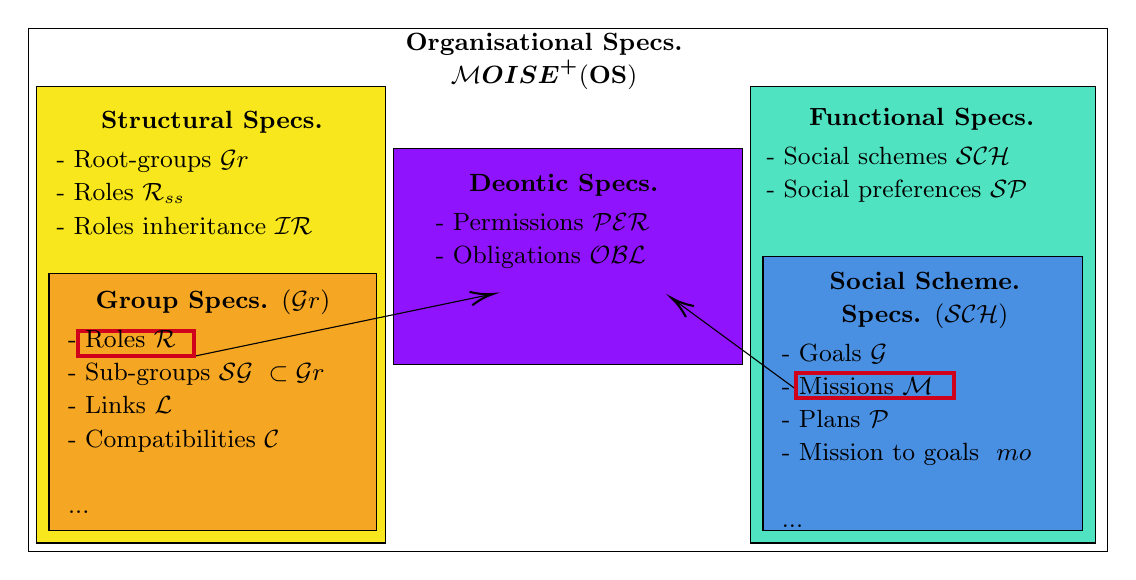
\begin{tikzpicture}[x=0.75pt,y=0.75pt,yscale=-1,xscale=1]
%uncomment if require: \path (0,1656); %set diagram left start at 0, and has height of 1656

%Shape: Rectangle [id:dp6756844921493015] 
\draw  [fill={rgb, 255:red, 248; green, 231; blue, 28 }  ,fill opacity=1 ] (46,1204) -- (214,1204) -- (214,1424) -- (46,1424) -- cycle ;
%Shape: Rectangle [id:dp3759944257810566] 
\draw  [fill={rgb, 255:red, 80; green, 227; blue, 194 }  ,fill opacity=1 ] (390,1204) -- (556,1204) -- (556,1424) -- (390,1424) -- cycle ;
%Shape: Rectangle [id:dp28244406216006945] 
\draw  [fill={rgb, 255:red, 144; green, 19; blue, 254 }  ,fill opacity=1 ] (218,1234) -- (386,1234) -- (386,1338) -- (218,1338) -- cycle ;
%Shape: Rectangle [id:dp32232123359581766] 
\draw   (42,1176) -- (562,1176) -- (562,1428) -- (42,1428) -- cycle ;
%Shape: Rectangle [id:dp7605706269262755] 
\draw  [fill={rgb, 255:red, 74; green, 144; blue, 226 }  ,fill opacity=1 ] (396,1286) -- (550,1286) -- (550,1418) -- (396,1418) -- cycle ;
%Shape: Rectangle [id:dp33110985390647496] 
\draw   (52,1294) -- (210,1294) -- (210,1418) -- (52,1418) -- cycle ;
%Shape: Rectangle [id:dp8653560038381976] 
\draw  [fill={rgb, 255:red, 245; green, 166; blue, 35 }  ,fill opacity=1 ] (52,1294) -- (210,1294) -- (210,1418) -- (52,1418) -- cycle ;
%Straight Lines [id:da09781093164567278] 
\draw    (412,1350) -- (353.61,1307.18) ;
\draw [shift={(352,1306)}, rotate = 36.25] [color={rgb, 255:red, 0; green, 0; blue, 0 }  ][line width=0.75]    (10.93,-3.29) .. controls (6.95,-1.4) and (3.31,-0.3) .. (0,0) .. controls (3.31,0.3) and (6.95,1.4) .. (10.93,3.29)   ;
%Straight Lines [id:da3938396723807833] 
\draw    (122,1334) -- (264.04,1304.41) ;
\draw [shift={(266,1304)}, rotate = 168.23] [color={rgb, 255:red, 0; green, 0; blue, 0 }  ][line width=0.75]    (10.93,-3.29) .. controls (6.95,-1.4) and (3.31,-0.3) .. (0,0) .. controls (3.31,0.3) and (6.95,1.4) .. (10.93,3.29)   ;
%Shape: Rectangle [id:dp269311335478327] 
\draw  [color={rgb, 255:red, 208; green, 2; blue, 27 }  ,draw opacity=1 ][line width=1.5]  (66,1322) -- (122,1322) -- (122,1334) -- (66,1334) -- cycle ;
%Shape: Rectangle [id:dp7449860119164387] 
\draw  [color={rgb, 255:red, 208; green, 2; blue, 27 }  ,draw opacity=1 ][line width=1.5]  (412,1342) -- (488,1342) -- (488,1354) -- (412,1354) -- cycle ;


% Text Node
\draw (472.5,1237.41) node   [align=left] {\begin{minipage}[lt]{112.2pt}\setlength\topsep{0pt}
\begin{center}
\textbf{{\small Functional Specs.}}
\end{center}
{\small  - Social schemes $\displaystyle \mathcal{SCH}$}\\{\small  - Social preferences $\displaystyle \mathcal{SP}$}
\end{minipage}};
% Text Node
\draw (474,1355) node   [align=left] {\begin{minipage}[lt]{103.36pt}\setlength\topsep{0pt}
\begin{center}
\textbf{{\small Social Scheme.}}\\{\small \textbf{Specs. }$\displaystyle (\mathcal{SCH})$}
\end{center}
{\small  - Goals $\displaystyle \mathcal{G}$}\\{\small  - Missions $\displaystyle \mathcal{M}$}\\{\small  - Plans $\displaystyle \mathcal{P}$}\\{\small  - Mission to goals \ $\displaystyle mo$}\\\\{\small  ...}
\end{minipage}};
% Text Node
\draw (131,1356) node   [align=left] {\begin{minipage}[lt]{104.72pt}\setlength\topsep{0pt}
\begin{center}
{\small \textbf{Group Specs. }$\displaystyle (\mathcal{G} r)$}
\end{center}
{\small  - Roles $\displaystyle \mathcal{R}$}\\{\small  - Sub-groups $\displaystyle \mathcal{SG} \ \subset \mathcal{G} r$}\\{\small  - Links $\displaystyle \mathcal{L}$}\\{\small  - Compatibilities $\displaystyle \mathcal{C}$}\\\\{\small  ...}
\end{minipage}};
% Text Node
\draw (181,1177) node [anchor=north west][inner sep=0.75pt]   [align=left] {\begin{minipage}[lt]{162.41pt}\setlength\topsep{0pt}
\begin{center}
{\small \textbf{Organisational Specs. }$\displaystyle \mathcal{M}\boldsymbol{OISE^{+}}$($\displaystyle \mathbf{OS}$)}
\end{center}

\end{minipage}};
% Text Node
\draw (300,1269.09) node   [align=left] {\begin{minipage}[lt]{92.48pt}\setlength\topsep{0pt}
\begin{center}
\textbf{{\small Deontic Specs.}}
\end{center}
{\small  - Permissions $\displaystyle \mathcal{PER}$}\\{\small  - Obligations $\displaystyle \mathcal{OBL}$}
\end{minipage}};
% Text Node
\draw (130.5,1245.69) node   [align=left] {\begin{minipage}[lt]{112.2pt}\setlength\topsep{0pt}
\begin{center}
\textbf{{\small Structural Specs.}}
\end{center}
{\small  - Root-groups $\displaystyle \mathcal{G} r$}\\{\small  - Roles $\displaystyle \mathcal{R}_{ss}$}\\{\small  - Roles inheritance $\displaystyle \mathcal{IR}$}
\end{minipage}};


\end{tikzpicture}
    \caption{A synthetic view of the $\mathcal{M}OISE^+$ model}
    \label{fig:moise_model}
\end{figure}

As illustrated in \autoref{fig:moise_model},
%
$\mathcal{M}OISE^+$~\citep{Hubner2002} provides an advanced formal description for an organization without incompatibilities with MARL, especially for formal description of agents' policies. It takes into account explicitly the social aspects between agents where \textquote{AGR} focuses on the integration of standards oriented towards design. Additionally, it provides a sufficiently detailed vision of organization to be understood at different point of views.
Based on $\mathcal{M}OISE^+$~\citep{Hubner2007} formalism, we only give the minimal elements of the formalism we used for our approach.

\paragraph{\textbf{Organization specifications (OS)}}: $\mathcal{OS} = \langle \mathcal{SS}, \mathcal{FS}, \mathcal{DS} \rangle$, the set of all organization specifications, where $\mathcal{SS}$ are the \textbf{Structural Specifications}, $\mathcal{FS}$ are the \textbf{Functional Specifications}, and $\mathcal{DS}$ are the \textbf{Deontic Specifications}

\paragraph{\textbf{Structural Specifications (SS)}}: $\mathcal{SS} = \langle \mathcal{R}, \mathcal{IR}, \mathcal{G} \rangle$, where:

\begin{itemize}

    \item $\mathcal{R}_{ss}$: the set of all roles (denoted $\rho \in \mathcal{R}$);

    \item $\mathcal{IR}: \mathcal{R} \rightarrow \mathcal{R}$: the inheritance relation between roles ($\mathcal{IR}(\rho_1) = \rho_2$ means $\rho_1$ inherits from $\rho_2$ also denoted $\rho_1 \sqsubset \rho_2$);

    \item $RG \subseteq GR$ the set of root groups, $GR = \langle \mathcal{R}, \mathcal{SG}, \mathcal{L}^{intra}, \mathcal{L}^{inter}, \mathcal{C}^{intra}, \mathcal{C}^{inter}, np, ng \rangle$, the set of all groups, where

          \begin{itemize}

              \item $\mathcal{R} \subseteq \mathcal{R}_{ss}$: the set of non-abstract roles;

              \item $\mathcal{SG} \subseteq \mathcal{GR}$: the set of sub-groups;

              \item $\mathcal{L} = \mathcal{R} \cross \mathcal{R} \cross \mathcal{TL}$: the set of links. A link is a 3-tuple $(\rho_s,\rho_d,t) \in \mathcal{L}$ (also denoted as a predicate $link(\rho_s,\rho_d,t))$, where $\rho_{s}$ is the source role, $\rho_{d}$ is the destination role, and $t \in \mathcal{TL}, \mathcal{TL} = \{acq, com, aut\}$ is the link type;
                    \begin{itemize}
                        \item If $t = acq$ (acquaintance), the agents playing the source role $\rho_{\mathrm{s}}$ are allowed to have a representation of the agents playing the destination role $\rho_{d}$;
                        \item If $t = com$ (communication), the $\rho_{\mathrm{s}}$ agents are allowed to communicate with $\rho_{d}$ agents;
                        \item If $t = aut$ (authority), the $\rho_{\mathrm{s}}$ agents are allowed to have authority on $\rho_{d}$ agents. It requires an acquaintance and communication link.
                    \end{itemize}
              \item $\mathcal{L}^{intra} \subseteq \mathcal{L}$: the set of intra-group links;
              \item $\mathcal{L}^{inter} \subseteq \mathcal{L}$: the set of inter-group links;

              \item $\mathcal{C} = \mathcal{R} \cross \mathcal{R}$: the set of compatibilities. A compatibility is a couple $(a,b) \in \mathcal{C}$ (also denoted $\rho_a \bowtie \rho_b$), means agents playing role $\rho_a \in \mathcal{R}$ can also play role $\rho_b \in \mathcal{R}$;
              \item $\mathcal{C}^{intra} \subseteq \mathcal{C}$: the set of intra-group compatibilities;
              \item $\mathcal{C}^{inter} \subseteq \mathcal{C}$: the set of inter-group compatibilities;

              \item $np: \mathcal{R} \rightarrow \mathbb{N} \times \mathbb{N}$: the relation giving the cardinality of agents adopting a role;
              \item $ng: \mathcal{SG} \rightarrow \mathbb{N} \times \mathbb{N}$: the relation giving the cardinality of each sub-group.

          \end{itemize}

\end{itemize}

\paragraph{\textbf{Functional Specifications (FS)}}: $\mathcal{FS} = \langle \mathcal{SCH}, \mathcal{PO} \rangle$, where:

\begin{itemize}
    \item $\mathcal{SCH} = \langle\mathcal{G}, \mathcal{M}, \mathcal{P}, mo, nm \rangle$: the set of \textbf{social scheme}, where:
          \begin{itemize}
              \item $\mathcal{G}$ is the set of global goal;

              \item $\mathcal{M}$ is the set of mission labels;
              \item $\mathcal{P} = \langle \mathcal{G}, \{\mathcal{G}\}^s, OP, [0,1] \rangle, s \in \mathbb{N}^*$ is the set of plans that builds the tree structure of the goals.
              %
              A plan $p \in \mathcal{P}$ is 4-tuple $p=(g_f,\{g_i\}_{0 \leq i \leq s}, op, p), g_f \in \mathcal{G}, g_i \in \mathcal{G}, op \in OP, OP = \{sequence, choice, parallel\}, p \in [0,1]$, meaning that the goal $g_f$ is achieved if some of the sub-goals $g_i$ are achieved with a success probability $p$ and according to the operator $op$:
              %
              \begin{itemize}
                \item if $op = sequence$, the $g_i$ can only be achieved in the same order sequentially;
                \item if $op = choice$, only one of the $g_i$ has to be achieved;
                \item if $op = parallel$, the $g_i$ can only be achieved sequentially or simultaneously.
              \end{itemize}

              \item $mo: \mathcal{M} \rightarrow \mathbb{P}(\mathcal{G})$: specifies the set of goals a mission is associated to;
              \item $nm: \mathcal{M} \rightarrow \mathbb{N} \times \mathbb{N}$ the cardinality of agents committed for each mission.
          \end{itemize}
    \item $\mathcal{PO}: \mathcal{M} \cross \mathcal{M}$: the set of \textbf{preference order}. A preference order is couple $(m_1, m_2), m_1 \in \mathcal{M}, m_2 \in \mathcal{M}$ (also denoted $m_{1} \prec m_{2}$) meaning that if there is a moment when an agent is permitted to commit to $m_{1}$ and also $m_{2}$, it has a social preference for committing to $m_{1}$.
\end{itemize}

\paragraph{\textbf{Deontic Specifications (DS)}}: $\mathcal{DS} = \langle \mathcal{OBL},\mathcal{PER} \rangle$, the set of deontic specifications, where:

\begin{itemize}
    \item $\mathcal{TC}$: the set of \textbf{time constraints}. A time constraint $tc \in \mathcal{TC}$ specifies a set of periods during which a permission or obligation is valid ($Any \in \mathcal{TC}$ means everytime);
    \item $\mathcal{OBL}: \mathcal{R} \cross \mathcal{M} \cross \mathcal{TC}$: the set of \textbf{obligations}. An obligation is a 3-tuple $(\rho_a,m,tc)$ (aslo denoted $obl(\rho_a,m,tc)$) meaning an agent playing role $\rho_a \in \mathcal{R}$ is obliged to commit on mission $m \in \mathcal{M}$ for a given time constraint $tc \in \mathcal{TC}$;
    \item $\mathcal{PER}$: the set of \textbf{permissions}. A permission is a 3-tuple $(\rho_a,m,tc)$ (aslo denoted $per(\rho_a,m,tc)$) meaning an agent playing role $\rho_a \in \mathcal{R}$ is permitted to commit on mission $m \in \mathcal{M}$ for a given time constraint $tc \in \mathcal{TC}$;
\end{itemize}

\

\noindent Organizational specifications applied to agents are roles and goals (as missions) through permissions or obligations. Indeed, the other structural specifications such as compatibilities or links are inherent to roles. Similarly, we consider that the goals, the missions, and their mapping ($mo$) are enough to also link all of the other functional specifications such as plans, cardinalities, or preference orders.
Consequently, we consider it is sufficient to take into account roles, missions (goal and mapping) and permissions/obligations when linking $\mathcal{M}OISE^+$ with Dec-POMDP. 


\subsection{Linking $\mathcal{M}OISE^+$ with MARL}

\begin{figure}[h!]
    \centering
    \tikzset{every picture/.style={line width=0.75pt}} %set default line width to 0.75pt        

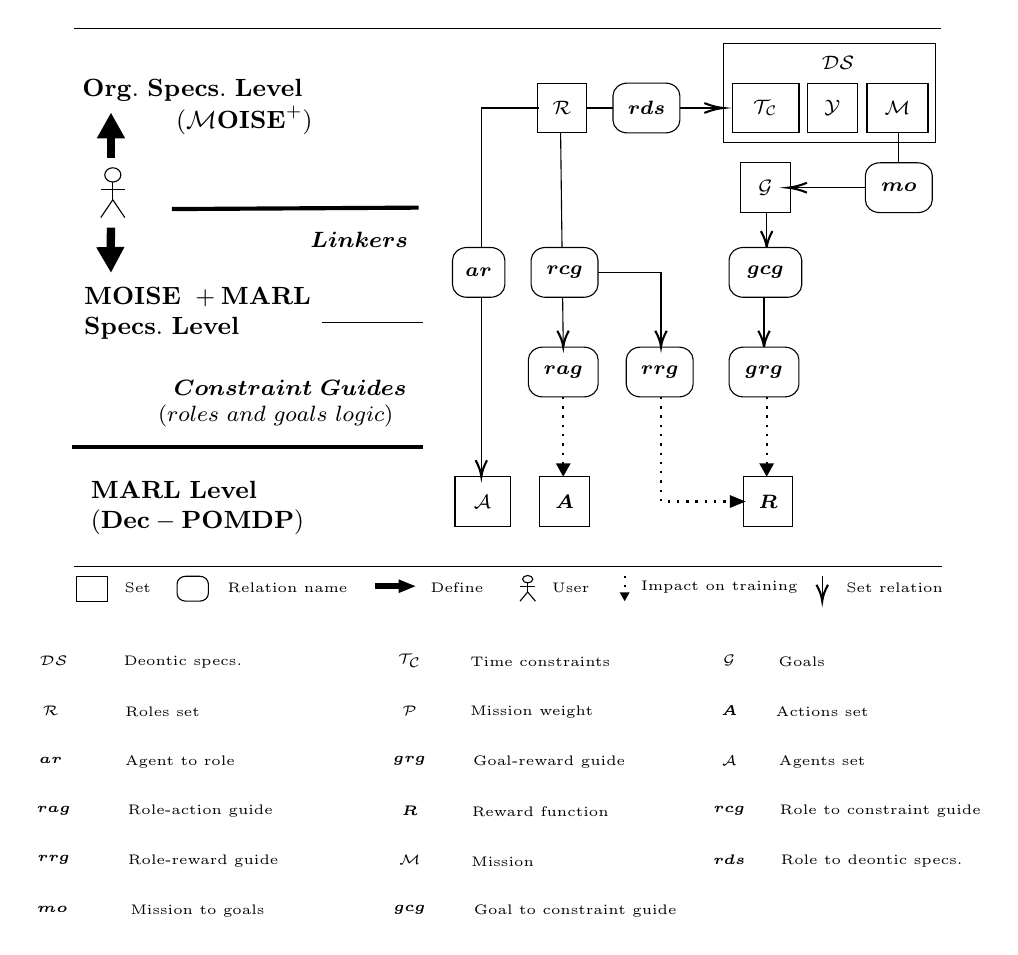
\begin{tikzpicture}[x=0.75pt,y=0.75pt,yscale=-1.2,xscale=1.4]
    %uncomment if require: \path (0,2584); %set diagram left start at 0, and has height of 2584

    %Straight Lines [id:da4973066741986565] 
    \draw [line width=1.5]    (118.21,2302.58) -- (203.1,2302) ;
    %Straight Lines [id:da14807114776731778] 
    \draw    (368.35,2272) -- (368.35,2294) -- (332.16,2294) ;
    \draw [shift={(330.16,2294)}, rotate = 360] [color={rgb, 255:red, 0; green, 0; blue, 0 }  ][line width=0.75]    (6.56,-1.97) .. controls (4.17,-0.84) and (1.99,-0.18) .. (0,0) .. controls (1.99,0.18) and (4.17,0.84) .. (6.56,1.97)   ;
    %Straight Lines [id:da16285043353898754] 
    \draw [line width=1.5]    (83.88,2398) -- (204.61,2398) ;
    %Straight Lines [id:da6299512000169913] 
    \draw    (169.94,2348) -- (204.61,2348) ;
    %Straight Lines [id:da64750232417664] 
    \draw    (84.65,2446) -- (383.15,2446) ;
    %Straight Lines [id:da35895220906699743] 
    \draw    (84.65,2230) -- (383,2230) ;
    %Straight Lines [id:da715014372569708] 
    \draw    (244.68,2262) -- (224.68,2262) -- (224.68,2408) ;
    \draw [shift={(224.68,2410)}, rotate = 270] [color={rgb, 255:red, 0; green, 0; blue, 0 }  ][line width=0.75]    (6.56,-1.97) .. controls (4.17,-0.84) and (1.99,-0.18) .. (0,0) .. controls (1.99,0.18) and (4.17,0.84) .. (6.56,1.97)   ;
    %Straight Lines [id:da71870438525014] 
    \draw    (251.96,2328) -- (286.51,2328) -- (286.51,2356) ;
    \draw [shift={(286.51,2358)}, rotate = 270] [color={rgb, 255:red, 0; green, 0; blue, 0 }  ][line width=0.75]    (6.56,-1.97) .. controls (4.17,-0.84) and (1.99,-0.18) .. (0,0) .. controls (1.99,0.18) and (4.17,0.84) .. (6.56,1.97)   ;
    %Straight Lines [id:da6006267784187092] 
    \draw [line width=0.75]  [dash pattern={on 0.84pt off 2.51pt}]  (252.87,2378) -- (252.87,2407) ;
    \draw [shift={(252.87,2410)}, rotate = 270] [fill={rgb, 255:red, 0; green, 0; blue, 0 }  ][line width=0.08]  [draw opacity=0] (5.36,-2.57) -- (0,0) -- (5.36,2.57) -- cycle    ;
    %Straight Lines [id:da8743336135156266] 
    \draw    (322.88,2304) -- (322.88,2316) ;
    \draw [shift={(322.88,2318)}, rotate = 270] [color={rgb, 255:red, 0; green, 0; blue, 0 }  ][line width=0.75]    (6.56,-1.97) .. controls (4.17,-0.84) and (1.99,-0.18) .. (0,0) .. controls (1.99,0.18) and (4.17,0.84) .. (6.56,1.97)   ;
    %Straight Lines [id:da14641229967966152] 
    \draw [line width=0.75]  [dash pattern={on 0.84pt off 2.51pt}]  (322.88,2378) -- (322.88,2407) ;
    \draw [shift={(322.88,2410)}, rotate = 270] [fill={rgb, 255:red, 0; green, 0; blue, 0 }  ][line width=0.08]  [draw opacity=0] (5.36,-2.57) -- (0,0) -- (5.36,2.57) -- cycle    ;
    %Straight Lines [id:da9260929933425808] 
    \draw [line width=0.75]  [dash pattern={on 0.84pt off 2.51pt}]  (286.51,2378) -- (286.51,2420) -- (312.61,2420) ;
    \draw [shift={(315.61,2420)}, rotate = 180] [fill={rgb, 255:red, 0; green, 0; blue, 0 }  ][line width=0.08]  [draw opacity=0] (5.36,-2.57) -- (0,0) -- (5.36,2.57) -- cycle    ;
    %Straight Lines [id:da3057006030233673] 
    \draw [line width=0.75]  [dash pattern={on 0.84pt off 2.51pt}]  (274,2449.7) -- (274,2457) ;
    \draw [shift={(274,2460)}, rotate = 270] [fill={rgb, 255:red, 0; green, 0; blue, 0 }  ][line width=0.08]  [draw opacity=0] (3.57,-1.72) -- (0,0) -- (3.57,1.72) -- cycle    ;
    %Straight Lines [id:da07288166228322246] 
    \draw    (342,2449.98) -- (342,2458) ;
    \draw [shift={(342,2460)}, rotate = 270] [color={rgb, 255:red, 0; green, 0; blue, 0 }  ][line width=0.75]    (6.56,-1.97) .. controls (4.17,-0.84) and (1.99,-0.18) .. (0,0) .. controls (1.99,0.18) and (4.17,0.84) .. (6.56,1.97)   ;
    %Shape: Ellipse [id:dp8508274348425935] 
    \draw   (95.09,2288.86) .. controls (95.09,2287.28) and (96.33,2286) .. (97.85,2286) .. controls (99.38,2286) and (100.62,2287.28) .. (100.62,2288.86) .. controls (100.62,2290.44) and (99.38,2291.71) .. (97.85,2291.71) .. controls (96.33,2291.71) and (95.09,2290.44) .. (95.09,2288.86) -- cycle ;
    %Straight Lines [id:da3825450168053828] 
    \draw    (97.85,2291.71) -- (97.85,2298.86) ;
    %Straight Lines [id:da521321206042058] 
    \draw    (97.85,2298.86) -- (93.71,2306) ;
    %Straight Lines [id:da055514206493922025] 
    \draw    (97.85,2298.86) -- (102,2306) ;
    %Straight Lines [id:da8996496708356774] 
    \draw    (102,2294.57) -- (93.71,2294.57) ;

    %Straight Lines [id:da31678488015771755] 
    \draw [line width=2.25]    (188,2454) -- (196.97,2454) ;
    \draw [shift={(201.97,2454)}, rotate = 180] [fill={rgb, 255:red, 0; green, 0; blue, 0 }  ][line width=0.08]  [draw opacity=0] (5.72,-2.75) -- (0,0) -- (5.72,2.75) -- cycle    ;
    %Shape: Ellipse [id:dp3927356466672782] 
    \draw   (238.88,2451.17) .. controls (238.88,2450.36) and (239.67,2449.7) .. (240.64,2449.7) .. controls (241.61,2449.7) and (242.4,2450.36) .. (242.4,2451.17) .. controls (242.4,2451.99) and (241.61,2452.65) .. (240.64,2452.65) .. controls (239.67,2452.65) and (238.88,2451.99) .. (238.88,2451.17) -- cycle ;
    %Straight Lines [id:da3365602555559104] 
    \draw    (240.64,2452.65) -- (240.64,2456.32) ;
    %Straight Lines [id:da7990875235744026] 
    \draw    (240.64,2456.32) -- (238,2460) ;
    %Straight Lines [id:da23945649338821617] 
    \draw    (240.64,2456.32) -- (243.28,2460) ;
    %Straight Lines [id:da11927353559661591] 
    \draw    (243.28,2454.12) -- (238,2454.12) ;

    %Straight Lines [id:da5816423191130675] 
    \draw    (251.96,2272) -- (252.85,2356) ;
    \draw [shift={(252.87,2358)}, rotate = 269.39] [color={rgb, 255:red, 0; green, 0; blue, 0 }  ][line width=0.75]    (6.56,-1.97) .. controls (4.17,-0.84) and (1.99,-0.18) .. (0,0) .. controls (1.99,0.18) and (4.17,0.84) .. (6.56,1.97)   ;
    %Straight Lines [id:da9310455126832857] 
    \draw    (321.97,2338) -- (321.97,2356) ;
    \draw [shift={(321.97,2358)}, rotate = 270] [color={rgb, 255:red, 0; green, 0; blue, 0 }  ][line width=0.75]    (6.56,-1.97) .. controls (4.17,-0.84) and (1.99,-0.18) .. (0,0) .. controls (1.99,0.18) and (4.17,0.84) .. (6.56,1.97)   ;
    %Shape: Rectangle [id:dp293492578719597] 
    \draw   (120,2453) .. controls (120,2451.34) and (121.34,2450) .. (123,2450) -- (127.72,2450) .. controls (129.37,2450) and (130.72,2451.34) .. (130.72,2453) -- (130.72,2457) .. controls (130.72,2458.66) and (129.37,2460) .. (127.72,2460) -- (123,2460) .. controls (121.34,2460) and (120,2458.66) .. (120,2457) -- cycle ;
    %Straight Lines [id:da33566712615128225] 
    \draw    (261.05,2262) -- (306,2262) ;
    \draw [shift={(308,2262)}, rotate = 180] [color={rgb, 255:red, 0; green, 0; blue, 0 }  ][line width=0.75]    (6.56,-1.97) .. controls (4.17,-0.84) and (1.99,-0.18) .. (0,0) .. controls (1.99,0.18) and (4.17,0.84) .. (6.56,1.97)   ;
    %Shape: Rectangle [id:dp28383270948937667] 
    \draw   (308,2236) -- (381.08,2236) -- (381.08,2276) -- (308,2276) -- cycle ;
    %Straight Lines [id:da18020989903965012] 
    \draw [line width=3]    (97.22,2282) -- (97.22,2270) ;
    \draw [shift={(97.22,2264)}, rotate = 90] [fill={rgb, 255:red, 0; green, 0; blue, 0 }  ][line width=0.08]  [draw opacity=0] (10.18,-4.89) -- (0,0) -- (10.18,4.89) -- cycle    ;
    %Straight Lines [id:da018421338049046554] 
    \draw [line width=3]    (97.22,2310) -- (97.11,2322.37) ;
    \draw [shift={(97.22,2328)}, rotate = 268.86] [fill={rgb, 255:red, 0; green, 0; blue, 0 }  ][line width=0.08]  [draw opacity=0] (10.18,-4.89) -- (0,0) -- (10.18,4.89) -- cycle    ;
    %Shape: Rectangle [id:dp7281037051878541] 
    \draw   (85.42,2450) -- (96.13,2450) -- (96.13,2460) -- (85.42,2460) -- cycle ;

    % Text Node
    \draw (362,2544.5) node  [font=\tiny] [align=left] {Role to constraint guide};
    % Text Node
    \draw (342,2524.5) node  [font=\tiny] [align=left] {Agents set};
    % Text Node
    \draw (342,2504.5) node  [font=\tiny] [align=left] {Actions set};
    % Text Node
    \draw (257,2584.5) node  [font=\tiny] [align=left] {Goal to constraint guide};
    % Text Node
    \draw (335,2484.5) node  [font=\tiny] [align=left] {Goals};
    % Text Node
    \draw (359,2564.5) node  [font=\tiny] [align=left] {Role to deontic specs.};
    % Text Node
    \draw (232,2564.5) node  [font=\tiny] [align=left] {Mission};
    % Text Node
    \draw (245,2544.5) node  [font=\tiny] [align=left] {Reward function};
    % Text Node
    \draw (248,2524.5) node  [font=\tiny] [align=left] {Goal-reward guide};
    % Text Node
    \draw (242,2504.5) node  [font=\tiny] [align=left] {Mission weight};
    % Text Node
    \draw (245,2484.5) node  [font=\tiny] [align=left] {Time constraints};
    % Text Node
    \draw (127,2584.5) node  [font=\tiny] [align=left] {Mission to goals};
    % Text Node
    \draw (129,2564.5) node  [font=\tiny] [align=left] {Role-reward guide};
    % Text Node
    \draw (128,2544.5) node  [font=\tiny] [align=left] {Role-action guide};
    % Text Node
    \draw (121,2524.5) node  [font=\tiny] [align=left] {Agent to role};
    % Text Node
    \draw (115,2504.5) node  [font=\tiny] [align=left] {Roles set};
    % Text Node
    \draw (122,2484.5) node  [font=\tiny] [align=left] {Deontic specs.};
    % Text Node
    \draw (310,2544) node  [font=\tiny] [align=left] {$\displaystyle \boldsymbol{rcg}$};
    % Text Node
    \draw (200,2504) node  [font=\tiny] [align=left] {$\displaystyle \mathcal{P}$};
    % Text Node
    \draw (200,2484) node  [font=\tiny] [align=left] {$\displaystyle \mathcal{T_{C}}$};
    % Text Node
    \draw (200,2564) node  [font=\tiny] [align=left] {$\displaystyle \mathcal{M}$};
    % Text Node
    \draw (77.5,2484) node  [font=\tiny] [align=left] {$\displaystyle \mathcal{DS}$};
    % Text Node
    \draw (310,2564) node  [font=\tiny] [align=left] {$\displaystyle \boldsymbol{rds}$};
    % Text Node
    \draw (310,2504) node  [font=\tiny] [align=left] {$\displaystyle \boldsymbol{A}$};
    % Text Node
    \draw (200,2544) node  [font=\tiny] [align=left] {$\displaystyle \boldsymbol{R}$};
    % Text Node
    \draw (310,2524) node  [font=\tiny] [align=left] {$\displaystyle \mathcal{A}$};
    % Text Node
    \draw (200,2524) node  [font=\tiny] [align=left] {$\displaystyle \boldsymbol{grg}$};
    % Text Node
    \draw (77.5,2564) node  [font=\tiny] [align=left] {$\displaystyle \boldsymbol{rrg}$};
    % Text Node
    \draw (77.5,2544) node  [font=\tiny] [align=left] {$\displaystyle \boldsymbol{rag}$};
    % Text Node
    \draw (200,2584) node  [font=\tiny] [align=left] {$\displaystyle \boldsymbol{gcg}$};
    % Text Node
    \draw (76.5,2524) node  [font=\tiny] [align=left] {$\displaystyle \boldsymbol{ar}$};
    % Text Node
    \draw (77,2584) node  [font=\tiny] [align=left] {$\displaystyle \boldsymbol{mo}$};
    % Text Node
    \draw (76.5,2504) node  [font=\tiny] [align=left] {$\displaystyle \mathcal{R}$};
    % Text Node
    \draw (310,2484) node  [font=\tiny] [align=left] {$\displaystyle \mathcal{G}$};


    % Text Node
    \draw  [fill={rgb, 255:red, 255; green, 255; blue, 255 }  ,fill opacity=1 ]  (241.82,2323) .. controls (241.82,2320.24) and (244.06,2318) .. (246.82,2318) -- (259.82,2318) .. controls (262.58,2318) and (264.82,2320.24) .. (264.82,2323) -- (264.82,2333) .. controls (264.82,2335.76) and (262.58,2338) .. (259.82,2338) -- (246.82,2338) .. controls (244.06,2338) and (241.82,2335.76) .. (241.82,2333) -- cycle  ;
    \draw (253.32,2328) node  [font=\scriptsize] [align=left] {$\displaystyle \boldsymbol{rcg}$};
    % Text Node
    \draw    (337,2252) -- (354,2252) -- (354,2272) -- (337,2272) -- cycle  ;
    \draw (345.5,2262) node  [font=\scriptsize] [align=left] {$\displaystyle \mathcal{Y}$};
    % Text Node
    \draw    (311,2252) -- (334,2252) -- (334,2272) -- (311,2272) -- cycle  ;
    \draw (322.5,2262) node  [font=\scriptsize] [align=left] {$\displaystyle \mathcal{T_{C}}$};
    % Text Node
    \draw    (357.39,2252) -- (378.39,2252) -- (378.39,2272) -- (357.39,2272) -- cycle  ;
    \draw (367.89,2262) node  [font=\scriptsize] [align=left] {$\displaystyle \mathcal{M}$};
    % Text Node
    \draw (347.43,2244) node  [font=\scriptsize] [align=left] {$\displaystyle \mathcal{DS}$};
    % Text Node
    \draw  [fill={rgb, 255:red, 255; green, 255; blue, 255 }  ,fill opacity=1 ]  (270,2257) .. controls (270,2254.24) and (272.24,2252) .. (275,2252) -- (288,2252) .. controls (290.76,2252) and (293,2254.24) .. (293,2257) -- (293,2267) .. controls (293,2269.76) and (290.76,2272) .. (288,2272) -- (275,2272) .. controls (272.24,2272) and (270,2269.76) .. (270,2267) -- cycle  ;
    \draw (281.5,2262) node  [font=\scriptsize] [align=left] {$\displaystyle \boldsymbol{rds}$};
    % Text Node
    \draw (158,2454.5) node  [font=\tiny] [align=left] {Relation name};
    % Text Node
    \draw (106.46,2454.5) node  [font=\tiny] [align=left] {Set};
    % Text Node
    \draw (255.47,2454.5) node  [font=\tiny] [align=left] {User};
    % Text Node
    \draw (216.32,2454.5) node  [font=\tiny] [align=left] {Define};
    % Text Node
    \draw (366.91,2454.5) node  [font=\tiny] [align=left] {Set relation};
    % Text Node
    \draw (306.61,2454.5) node  [font=\tiny] [align=left] {Impact on training};
    % Text Node
    \draw    (244.82,2410) -- (261.82,2410) -- (261.82,2430) -- (244.82,2430) -- cycle  ;
    \draw (253.32,2420) node  [font=\scriptsize] [align=left] {$\displaystyle \boldsymbol{A}$};
    % Text Node
    \draw    (314.84,2410) -- (331.84,2410) -- (331.84,2430) -- (314.84,2430) -- cycle  ;
    \draw (323.34,2420) node  [font=\scriptsize] [align=left] {$\displaystyle \boldsymbol{R}$};
    % Text Node
    \draw    (215.63,2410) -- (234.63,2410) -- (234.63,2430) -- (215.63,2430) -- cycle  ;
    \draw (225.13,2420) node  [font=\scriptsize] [align=left] {$\displaystyle \mathcal{A}$};
    % Text Node
    \draw  [fill={rgb, 255:red, 255; green, 255; blue, 255 }  ,fill opacity=1 ]  (309.97,2363) .. controls (309.97,2360.24) and (312.21,2358) .. (314.97,2358) -- (328.97,2358) .. controls (331.73,2358) and (333.97,2360.24) .. (333.97,2363) -- (333.97,2373) .. controls (333.97,2375.76) and (331.73,2378) .. (328.97,2378) -- (314.97,2378) .. controls (312.21,2378) and (309.97,2375.76) .. (309.97,2373) -- cycle  ;
    \draw (321.97,2368) node  [font=\scriptsize] [align=left] {$\displaystyle \boldsymbol{grg}$};
    % Text Node
    \draw    (274.56,2363) .. controls (274.56,2360.24) and (276.8,2358) .. (279.56,2358) -- (292.56,2358) .. controls (295.32,2358) and (297.56,2360.24) .. (297.56,2363) -- (297.56,2373) .. controls (297.56,2375.76) and (295.32,2378) .. (292.56,2378) -- (279.56,2378) .. controls (276.8,2378) and (274.56,2375.76) .. (274.56,2373) -- cycle  ;
    \draw (286.06,2368) node  [font=\scriptsize] [align=left] {$\displaystyle \boldsymbol{rrg}$};
    % Text Node
    \draw    (240.87,2363) .. controls (240.87,2360.24) and (243.11,2358) .. (245.87,2358) -- (259.87,2358) .. controls (262.63,2358) and (264.87,2360.24) .. (264.87,2363) -- (264.87,2373) .. controls (264.87,2375.76) and (262.63,2378) .. (259.87,2378) -- (245.87,2378) .. controls (243.11,2378) and (240.87,2375.76) .. (240.87,2373) -- cycle  ;
    \draw (252.87,2368) node  [font=\scriptsize] [align=left] {$\displaystyle \boldsymbol{rag}$};
    % Text Node
    \draw (156.15,2380.5) node  [font=\footnotesize] [align=left] {$\displaystyle  \begin{array}{{>{\displaystyle}l}}
                \ \ \boldsymbol{Constraint\ Guides} \\
                ( roles\ and\ goals\ logic)
            \end{array}$};
    % Text Node
    \draw  [fill={rgb, 255:red, 255; green, 255; blue, 255 }  ,fill opacity=1 ]  (309.93,2323) .. controls (309.93,2320.24) and (312.17,2318) .. (314.93,2318) -- (329.93,2318) .. controls (332.69,2318) and (334.93,2320.24) .. (334.93,2323) -- (334.93,2333) .. controls (334.93,2335.76) and (332.69,2338) .. (329.93,2338) -- (314.93,2338) .. controls (312.17,2338) and (309.93,2335.76) .. (309.93,2333) -- cycle  ;
    \draw (322.43,2328) node  [font=\scriptsize] [align=left] {$\displaystyle \boldsymbol{gcg}$};
    % Text Node
    \draw  [fill={rgb, 255:red, 255; green, 255; blue, 255 }  ,fill opacity=1 ]  (214.77,2323) .. controls (214.77,2320.24) and (217.01,2318) .. (219.77,2318) -- (227.77,2318) .. controls (230.53,2318) and (232.77,2320.24) .. (232.77,2323) -- (232.77,2333) .. controls (232.77,2335.76) and (230.53,2338) .. (227.77,2338) -- (219.77,2338) .. controls (217.01,2338) and (214.77,2335.76) .. (214.77,2333) -- cycle  ;
    \draw (223.77,2328) node  [font=\scriptsize] [align=left] {$\displaystyle \boldsymbol{ar}$};
    % Text Node
    \draw  [fill={rgb, 255:red, 255; green, 255; blue, 255 }  ,fill opacity=1 ]  (356.85,2289) .. controls (356.85,2286.24) and (359.08,2284) .. (361.85,2284) -- (374.85,2284) .. controls (377.61,2284) and (379.85,2286.24) .. (379.85,2289) -- (379.85,2299) .. controls (379.85,2301.76) and (377.61,2304) .. (374.85,2304) -- (361.85,2304) .. controls (359.08,2304) and (356.85,2301.76) .. (356.85,2299) -- cycle  ;
    \draw (368.35,2294) node  [font=\scriptsize] [align=left] {$\displaystyle \boldsymbol{mo}$};
    % Text Node
    \draw (127,2344.5) node  [font=\small] [align=left] {$\displaystyle  \begin{array}{{>{\displaystyle}l}}
                \mathbf{MOISE\ +MARL} \\
                \mathbf{Specs.\ Level}
            \end{array}$};
    % Text Node
    \draw (127,2422.5) node  [font=\small] [align=left] {$\displaystyle  \begin{array}{{>{\displaystyle}l}}
                \mathbf{MARL\ Level} \\
                \mathbf{(Dec-POMDP)}
            \end{array}$};
    % Text Node
    \draw    (243.91,2252) -- (260.91,2252) -- (260.91,2272) -- (243.91,2272) -- cycle  ;
    \draw (252.41,2262) node  [font=\scriptsize] [align=left] {$\displaystyle \mathcal{R}$};
    % Text Node
    \draw (182.64,2315) node  [font=\footnotesize] [align=left] {$\displaystyle \boldsymbol{Linkers}$};
    % Text Node
    \draw    (313.93,2284) -- (330.93,2284) -- (330.93,2304) -- (313.93,2304) -- cycle  ;
    \draw (322.43,2294) node  [font=\scriptsize] [align=left] {$\displaystyle \mathcal{G}$};
    % Text Node
    \draw (127,2261.5) node  [font=\small] [align=left] {$\displaystyle  \begin{array}{{>{\displaystyle}l}}
                \mathbf{{\displaystyle Org.\ Specs.\ Level}} \\
                {\displaystyle \ \ \ \ \ \ \ \ \ \ \ (\mathcal{M}\mathbf{OISE^+})}
            \end{array}$};


\end{tikzpicture}
    \caption{A minimal view of the MOISE+MARL framework:
        Users first define $\mathcal{M}OISE^+$ specifications, which include roles ($\mathcal{R}$) and missions ($\mathcal{M}$), both associated through $rds$. They then create MOISE+MARL specifications by first defining \textbf{Constraint guides} such as $rag$ and $rrg$ to specify role logic, and $grg$ for goal logic. 
        Next, \textbf{Linkers} are used to connect agents with roles through $ar$ and to link the logic of the constraint guides to the defined $\mathcal{M}OISE^+$ specifications. Once this is set up, roles can be assigned to agents, and the MARL framework updates accordingly during training.
    }
    \label{fig:mm_synthesis}
\end{figure}

\

\noindent The \textbf{Constraint Guides} are three new relations introduced to describe the logics of $\mathcal{M}OISE^+$ roles and goals in the Dec-POMDP formalism:
%
% \begin{itemize}
\begin{enumerate*}[label={\roman*) },itemjoin={; \quad}]
    
    \item \textbf{Role Action Guide} \quad $rag: H \times \Omega \rightarrow \mathcal{P}(A \times \mathbb{R})$, the relation that models a role as a set of rules which, for each pair consisting of a history $h \in H$ and an observation received by the agent $\omega \in \Omega$, associates expected actions $A \in \mathcal{P}(A)$ each associated with a constraint hardness $ch \in [0,1]$ ($ch = 1$ by default). By restricting the choice of the next action among those authorized, the agent is forced to adhere to the role's expected behavior
    \item \textbf{Role Reward Guide} \quad $rrg: H \times \Omega \times A \to \mathbb{R} = \{r_m \text{ if } a \notin A_\omega \text{, } rag(h, \omega) \allowbreak = \allowbreak A_\omega \times \mathbb{R} \text{, } h \in H; \text{ else } 0\}$, the relation that models a role by adding a penalty $r_m$ to the global reward if the last action chosen by the agent $a \in A$ is not authorized. This is intended to encourage the agent to adhere to the expected behavior of a role
    \item \textbf{Goal Reward Guide} \quad $grg: H \rightarrow \mathbb{R}$, the relation that models a goal as a soft constraint adding a reward bonus $r_b \in \mathbb{R}$ if the agent's history $h \in H$ contains a goal's characteristic sub-sequence $h_g \in H_g$, encouraging the agent to reach it.
\end{enumerate*}
% \end{itemize}

\

\noindent Finally, we introduce the \textbf{Linkers} to link the $\mathcal{M}OISE^+$ organizational specifications with constraint guides and agents:
%
% \begin{itemize}
\begin{enumerate*}[label={\roman*) },itemjoin={; \quad}]
    
    \item \textbf{Agent to Role} \quad $ar: \mathcal{A} \to \mathcal{R}$, the bijective relation linking an agent to a role;
    \item \textbf{Role to Constraint Guide} \quad $rcg: \mathcal{R} \rightarrow rag \cup rrg$, the relation associating each $\mathcal{M}OISE^+$ role to a $rag$ or $rrg$ relation, forcing/encouraging the agent to follow the expected actions for the role $\rho \in \mathcal{R}$;
    \item \textbf{Goal to Constraint Guide} \quad $gcg: \mathcal{G} \rightarrow grg$, the relation linking goals to $grg$ relations, representing goals as rewards in MARL.
\end{enumerate*}
% \end{itemize}

\paragraph{\textbf{Resolving the Dec-POMDP with MOISE+MARL}}

A MOISE+MARL model is formalized as $MM = \langle \mathcal{OS}, ar, rcg, gcg, rag, rrg, grg\rangle$.
Resolving the Dec-POMDP $d \in D$ with a $mm \in \mathcal{MM}$ model involves finding a joint policy $\pi^{j} = \{\pi^j_0,\pi^j_1\dots\pi^j_n\}$ that maximizes the state-value function $V^{\pi^{j}}$ (or reaches a minimum threshold), which represents the expected cumulative reward starting from an initial state $s \in S$ and following the joint policy $\pi^{j}$, applying successive joint actions $a^{j} \in A^n$ under additional constraint guides. The state-value is described in the case where agents act sequentially and cyclically (Agent Environment Cycle - AEC mode) in \hyperref[eq:single_value_function]{Definition 1}, adapting its definition for roles (in red) and missions (in blue), impacting the action space and reward. \autoref{fig:mm_synthesis} illustrates the links between $\mathcal{M}OISE^+$ and Dec-POMDP via the MOISE+MARL framework.


\begin{figure*}[h!]
    \label{eq:single_value_function}
    \raggedright
    \textbf{\textit{Definition 1} \quad State-Value function adapted to constraint guides in AEC:}
    
    \begin{scriptsize}
        \vspace{-0.6cm}
        \begin{gather*}
            V^{\pi^j}(s_t) = \hspace{-0.75cm}
            %
            \sum_{\textcolor{red}{ \substack{a_{t} \in A \text{ si } rn() < ch_{t}, \\
                        a_{t} \in A_{t} \text{ else}}
                }}{\hspace{-0.7cm} \pi_i(a_{t} | \omega_t)}
            %
            \sum_{s_{t+1} \in S}
            %    
            {\hspace{-0.1cm} T(s_{t+1} | s_t, a_{t})
            \Bigl[R(s_t,a_{t},s_{t+1}) + \hspace{-0.1cm}
            \textcolor{blue}{ \sum_{m \in \mathcal{M}_i}{ \hspace{-0.1cm} v_m(t) \frac{grg_m(h_{t+1})}{1 - p + \epsilon} } }
            + } \\
            {\textcolor{red}{(1-ch_t) \times rrg(\omega_t,a_{t+1})} + V^{\pi^j_{i+1 \ mod \ n}}(s_{t+1})\Bigr]}
        \end{gather*}
        %
        \vspace{-0.5cm}
        \textcolor{red}{\[\text{ \hspace{-0.1cm} With } rag(h_t, \omega_t) = A_{t} \times \mathbb{R} \text{, } \langle a_t, ch_{t} \rangle \in A_{t} \times \mathbb{R} \text{ ; } rn: \emptyset \to [0,1[ \text{, a uniform random function}\]}
        %
        \vspace{-0.6cm}
        \textcolor{blue}{
            \begin{gather*}
                \hspace{-0.001cm}
                \text{With } \omega_t = O(\omega_t | s_t, a_t) \text{ ; } h_t = \{h_0 = \langle \rangle, h_{t+1} = \langle h_t, \langle \omega_{t+1}, a_{t+1} \rangle \rangle \} \text{ ; } \epsilon \in \mathbb{R}_{>0} \text{ ; } grg_m(h) = 
            \end{gather*}
        }
        \vspace{-0.95cm}
        \textcolor{blue}{
            \begin{gather*}
                \hspace{-0.5cm} \sum_{\hspace{0.3cm}(grg_i,w_i) \in mo(m)}{\hspace{-0.9cm} w_i \times grg_i(h)}
                \text{ ; } v_m(t) = \{ 1 \text{ if } t \in t_c \text{ ; else } 0 \} \text{ ; } \mathcal{M}_i = \{m_j | \langle ar(i),m_j,t_c,p \rangle \in \mathcal{M}\}
            \end{gather*}
        }
        \vspace{-0.6cm}
    \end{scriptsize}
    
\end{figure*}


At any time $t \in \mathbb{N}$ (initially $t = 0$), the agent $i = t \ mod \ n$ is constrained to a role $\rho_i = ar(i)$. For each temporally valid deontic specification $d_i = rds(\rho_i) = \langle tc_i,y_i, m_i \rangle$, the agent is permitted (if $y_i = 0$) or obligated (if $y_i = 1$) to commit in mission $m_i \in \mathcal{M}, \mathcal{G}_{m_i} = mo(m_i)$, and $n \in \mathbb{N}$ the number of agents.
%
First, based on the received observation $\omega_t$, the agent must choose an action either: within the expected actions of the role $A_t$ if a random value is below the role constraint hardness $ch_t$; or within the set of all actions $A$ otherwise. If $ch_t = 1$, the role is strongly constrained for the agent and weakly otherwise.
%
Then, the action is applied to the current state $s_t$ to transition to the next state $s_{t+1}$, generate the next observation $\omega_{t+1}$, and yield a reward. The reward is the sum of the global reward with penalties and bonuses obtained from the organizational specifications: \quad i) the sum of the bonuses for goals associated with each temporally valid mission (via Goal Reward Guides), weighted by the associated value ($\frac{1}{1-p+\epsilon}$); \quad ii) the penalty associated with the role (via "Role Reward Guides") weighted by the role constraint hardness.
%
Finally, the cumulative reward calculation continues in the next state $s_{t+1} \in S$ with the next agent $(i+1) \ mod \ n$.



\subsection{Learning world models}

In RL, particularly under partial observability, \textbf{World Models}~\cite{ha2018recurrent} aim to approximate the transition and observation functions of a Partially Observable Markov Decision Process (POMDP) to enable planning, safe exploration, and efficient policy learning. This belongs to the \textit{model-based RL} (MBRL) paradigm~\cite{moerland2020model}. It is particularly usefull to capture an environment complexity in a simulation-like model automatically, yet lacking explicit environmental representation.

Let $\omega_t \in \Omega$ be the observation and $a_t \in \mathcal{A}$ the action at time $t$. The core of a world model is to approximates the \textbf{observable dynamics function} $\mathcal{T}: \Omega \times A \rightarrow \Omega$, that captures the hidden state transition and observable dynamics. Implementation of an observable dynamics function is often based on Recurrent Neural Network (RNN) such as or Long-Short Term Memory (LSTM)~\cite{hochreiter1997long} for temporal modeling. Yet, since observations are often too large in size to train a LSTM directly, an encoder $Enc: \Omega \rightarrow Z$ is often used to get reduced latent representation of observations, and a decoder $Dec: Z \rightarrow \Omega$ is used to decode predicted latent representation into a real observation.
\[
    z_t = Enc(\omega_t), \quad
    z_{t+1} = \mathcal{T}(z_t, a_t), \quad
    \hat{\omega}_{t+1} = Dec(z_{t+1}),
\]
where $\forall z \in Z, \omega \in \Omega, dim(z) \leq dim(\omega)$ considering an observation $\omega$ to be described as a vector.
Training minimizes the reconstruction loss $\|\omega_{t+1} - \hat{\omega}_{t+1}\|$ and a prediction loss in latent space.
%
In a multi-agent context, world modeling must accommodate decentralized dynamics~\cite{yang2021representation}. Then, then observable dynamics function treats joint-observation (as well as joint latent representation) and joint-action. In MAMAD, world models instantiate the simulation core of \hyperref[sec:modelling]{Modeling}, acting as digital twins.



\section{The MAMAD method}\label{sec:mamad}

\subsection{General overview of the method}

The MAMAD~\footnote{Source code and details of MAMAD are available at \url{https://github.com/julien6/MAMAD}} method is built around four main phases: (1) modeling the environment, goal, and organizational constraints according to the proposed framework, (2) learning policies using various MARL algorithms, (3) analyzing behaviors and inferring organizational specifications with a proposed method, and (4) developing and deploying the MAS. This approach guides the agent learning process while enforcing strict organizational constraints, ensuring the efficiency of the learned policies. The lifecycle of a MAMAD-designed MAS is illustrated in \autoref{fig:cycle}.

\begin{figure}[h!]
    \centering
    


\tikzset{every picture/.style={line width=0.75pt}} %set default line width to 0.75pt        

\begin{tikzpicture}[x=0.75pt,y=0.75pt,yscale=-1,xscale=1]
%uncomment if require: \path (0,3307); %set diagram left start at 0, and has height of 3307

%Shape: Smiley Face [id:dp29065495216725257] 
\draw  [line width=1.5]  (85.38,2800.11) .. controls (85.38,2797.7) and (87.16,2795.75) .. (89.36,2795.75) .. controls (91.55,2795.75) and (93.34,2797.7) .. (93.34,2800.11) .. controls (93.34,2802.52) and (91.55,2804.48) .. (89.36,2804.48) .. controls (87.16,2804.48) and (85.38,2802.52) .. (85.38,2800.11) -- cycle ; \draw  [line width=1.5]  (87.61,2798.63) .. controls (87.61,2798.39) and (87.78,2798.19) .. (88,2798.19) .. controls (88.22,2798.19) and (88.4,2798.39) .. (88.4,2798.63) .. controls (88.4,2798.87) and (88.22,2799.07) .. (88,2799.07) .. controls (87.78,2799.07) and (87.61,2798.87) .. (87.61,2798.63) -- cycle ; \draw  [line width=1.5]  (90.31,2798.63) .. controls (90.31,2798.39) and (90.49,2798.19) .. (90.71,2798.19) .. controls (90.93,2798.19) and (91.11,2798.39) .. (91.11,2798.63) .. controls (91.11,2798.87) and (90.93,2799.07) .. (90.71,2799.07) .. controls (90.49,2799.07) and (90.31,2798.87) .. (90.31,2798.63) -- cycle ; \draw  [line width=1.5]  (87.37,2801.86) .. controls (88.69,2803.02) and (90.02,2803.02) .. (91.35,2801.86) ;
%Shape: Rectangle [id:dp42672371521059915] 
\draw  [dash pattern={on 5.63pt off 4.5pt}][line width=1.5]  (74.03,2763.75) -- (192,2763.75) -- (192,2813.93) -- (74.03,2813.93) -- cycle ;
%Shape: Smiley Face [id:dp9817389082285293] 
\draw  [line width=1.5]  (144.45,2803.6) .. controls (144.45,2801.19) and (146.24,2799.24) .. (148.43,2799.24) .. controls (150.63,2799.24) and (152.41,2801.19) .. (152.41,2803.6) .. controls (152.41,2806.01) and (150.63,2807.97) .. (148.43,2807.97) .. controls (146.24,2807.97) and (144.45,2806.01) .. (144.45,2803.6) -- cycle ; \draw  [line width=1.5]  (146.68,2802.12) .. controls (146.68,2801.88) and (146.86,2801.68) .. (147.08,2801.68) .. controls (147.3,2801.68) and (147.48,2801.88) .. (147.48,2802.12) .. controls (147.48,2802.36) and (147.3,2802.56) .. (147.08,2802.56) .. controls (146.86,2802.56) and (146.68,2802.36) .. (146.68,2802.12) -- cycle ; \draw  [line width=1.5]  (149.39,2802.12) .. controls (149.39,2801.88) and (149.57,2801.68) .. (149.79,2801.68) .. controls (150.01,2801.68) and (150.18,2801.88) .. (150.18,2802.12) .. controls (150.18,2802.36) and (150.01,2802.56) .. (149.79,2802.56) .. controls (149.57,2802.56) and (149.39,2802.36) .. (149.39,2802.12) -- cycle ; \draw  [line width=1.5]  (146.44,2805.35) .. controls (147.77,2806.51) and (149.1,2806.51) .. (150.42,2805.35) ;
%Shape: Smiley Face [id:dp49419175504212776] 
\draw  [line width=1.5]  (179.09,2781.5) .. controls (179.09,2779.09) and (180.87,2777.13) .. (183.06,2777.13) .. controls (185.26,2777.13) and (187.04,2779.09) .. (187.04,2781.5) .. controls (187.04,2783.91) and (185.26,2785.86) .. (183.06,2785.86) .. controls (180.87,2785.86) and (179.09,2783.91) .. (179.09,2781.5) -- cycle ; \draw  [line width=1.5]  (181.31,2780.01) .. controls (181.31,2779.77) and (181.49,2779.58) .. (181.71,2779.58) .. controls (181.93,2779.58) and (182.11,2779.77) .. (182.11,2780.01) .. controls (182.11,2780.25) and (181.93,2780.45) .. (181.71,2780.45) .. controls (181.49,2780.45) and (181.31,2780.25) .. (181.31,2780.01) -- cycle ; \draw  [line width=1.5]  (184.02,2780.01) .. controls (184.02,2779.77) and (184.2,2779.58) .. (184.42,2779.58) .. controls (184.64,2779.58) and (184.81,2779.77) .. (184.81,2780.01) .. controls (184.81,2780.25) and (184.64,2780.45) .. (184.42,2780.45) .. controls (184.2,2780.45) and (184.02,2780.25) .. (184.02,2780.01) -- cycle ; \draw  [line width=1.5]  (181.07,2783.24) .. controls (182.4,2784.4) and (183.73,2784.4) .. (185.05,2783.24) ;
%Flowchart: Punched Tape [id:dp3565745198144521] 
\draw  [fill={rgb, 255:red, 255; green, 255; blue, 255 }  ,fill opacity=1 ] (291.67,2877.34) .. controls (291.67,2880.23) and (301.36,2882.58) .. (313.31,2882.58) .. controls (325.26,2882.58) and (334.95,2880.23) .. (334.95,2877.34) .. controls (334.95,2874.45) and (344.64,2872.11) .. (356.6,2872.11) .. controls (368.55,2872.11) and (378.24,2874.45) .. (378.24,2877.34) -- (378.24,2919.23) .. controls (378.24,2916.34) and (368.55,2913.99) .. (356.6,2913.99) .. controls (344.64,2913.99) and (334.95,2916.34) .. (334.95,2919.23) .. controls (334.95,2922.12) and (325.26,2924.46) .. (313.31,2924.46) .. controls (301.36,2924.46) and (291.67,2922.12) .. (291.67,2919.23) -- cycle ;
%Straight Lines [id:da23451091058783402] 
\draw [line width=1.5]    (320.63,2891.89) -- (349.47,2889.91) ;
\draw [shift={(352.46,2889.7)}, rotate = 176.08] [color={rgb, 255:red, 0; green, 0; blue, 0 }  ][line width=1.5]    (8.53,-2.57) .. controls (5.42,-1.09) and (2.58,-0.23) .. (0,0) .. controls (2.58,0.23) and (5.42,1.09) .. (8.53,2.57)   ;
%Straight Lines [id:da05993633349010663] 
\draw [line width=1.5]    (320.63,2894.07) -- (335.84,2901.48) ;
\draw [shift={(338.53,2902.79)}, rotate = 205.98] [color={rgb, 255:red, 0; green, 0; blue, 0 }  ][line width=1.5]    (8.53,-2.57) .. controls (5.42,-1.09) and (2.58,-0.23) .. (0,0) .. controls (2.58,0.23) and (5.42,1.09) .. (8.53,2.57)   ;
%Shape: Smiley Face [id:dp5316832937595011] 
\draw  [line width=1.5]  (312.91,2893.34) .. controls (312.91,2890.93) and (314.69,2888.98) .. (316.89,2888.98) .. controls (319.09,2888.98) and (320.87,2890.93) .. (320.87,2893.34) .. controls (320.87,2895.75) and (319.09,2897.7) .. (316.89,2897.7) .. controls (314.69,2897.7) and (312.91,2895.75) .. (312.91,2893.34) -- cycle ; \draw  [line width=1.5]  (315.14,2891.86) .. controls (315.14,2891.61) and (315.32,2891.42) .. (315.54,2891.42) .. controls (315.76,2891.42) and (315.94,2891.61) .. (315.94,2891.86) .. controls (315.94,2892.1) and (315.76,2892.29) .. (315.54,2892.29) .. controls (315.32,2892.29) and (315.14,2892.1) .. (315.14,2891.86) -- cycle ; \draw  [line width=1.5]  (317.85,2891.86) .. controls (317.85,2891.61) and (318.02,2891.42) .. (318.24,2891.42) .. controls (318.46,2891.42) and (318.64,2891.61) .. (318.64,2891.86) .. controls (318.64,2892.1) and (318.46,2892.29) .. (318.24,2892.29) .. controls (318.02,2892.29) and (317.85,2892.1) .. (317.85,2891.86) -- cycle ; \draw  [line width=1.5]  (314.9,2895.08) .. controls (316.23,2896.25) and (317.55,2896.25) .. (318.88,2895.08) ;
%Shape: Smiley Face [id:dp5491508300746957] 
\draw  [line width=1.5]  (338.38,2904.97) .. controls (338.38,2902.56) and (340.16,2900.61) .. (342.35,2900.61) .. controls (344.55,2900.61) and (346.33,2902.56) .. (346.33,2904.97) .. controls (346.33,2907.38) and (344.55,2909.34) .. (342.35,2909.34) .. controls (340.16,2909.34) and (338.38,2907.38) .. (338.38,2904.97) -- cycle ; \draw  [line width=1.5]  (340.6,2903.49) .. controls (340.6,2903.25) and (340.78,2903.05) .. (341,2903.05) .. controls (341.22,2903.05) and (341.4,2903.25) .. (341.4,2903.49) .. controls (341.4,2903.73) and (341.22,2903.93) .. (341,2903.93) .. controls (340.78,2903.93) and (340.6,2903.73) .. (340.6,2903.49) -- cycle ; \draw  [line width=1.5]  (343.31,2903.49) .. controls (343.31,2903.25) and (343.49,2903.05) .. (343.71,2903.05) .. controls (343.93,2903.05) and (344.1,2903.25) .. (344.1,2903.49) .. controls (344.1,2903.73) and (343.93,2903.93) .. (343.71,2903.93) .. controls (343.49,2903.93) and (343.31,2903.73) .. (343.31,2903.49) -- cycle ; \draw  [line width=1.5]  (340.36,2906.72) .. controls (341.69,2907.88) and (343.02,2907.88) .. (344.34,2906.72) ;
%Shape: Smiley Face [id:dp21362593128550156] 
\draw  [line width=1.5]  (352.64,2888.69) .. controls (352.64,2886.28) and (354.42,2884.32) .. (356.61,2884.32) .. controls (358.81,2884.32) and (360.59,2886.28) .. (360.59,2888.69) .. controls (360.59,2891.1) and (358.81,2893.05) .. (356.61,2893.05) .. controls (354.42,2893.05) and (352.64,2891.1) .. (352.64,2888.69) -- cycle ; \draw  [line width=1.5]  (354.86,2887.2) .. controls (354.86,2886.96) and (355.04,2886.77) .. (355.26,2886.77) .. controls (355.48,2886.77) and (355.66,2886.96) .. (355.66,2887.2) .. controls (355.66,2887.44) and (355.48,2887.64) .. (355.26,2887.64) .. controls (355.04,2887.64) and (354.86,2887.44) .. (354.86,2887.2) -- cycle ; \draw  [line width=1.5]  (357.57,2887.2) .. controls (357.57,2886.96) and (357.75,2886.77) .. (357.97,2886.77) .. controls (358.19,2886.77) and (358.36,2886.96) .. (358.36,2887.2) .. controls (358.36,2887.44) and (358.19,2887.64) .. (357.97,2887.64) .. controls (357.75,2887.64) and (357.57,2887.44) .. (357.57,2887.2) -- cycle ; \draw  [line width=1.5]  (354.62,2890.43) .. controls (355.95,2891.59) and (357.28,2891.59) .. (358.6,2890.43) ;
%Left Arrow [id:dp22187584774212898] 
\draw   (215,2804.55) -- (220.28,2802) -- (220.28,2803.27) -- (263.54,2803.27) -- (263.54,2805.82) -- (220.28,2805.82) -- (220.28,2807.09) -- cycle ;
%Left Arrow [id:dp1861077704673879] 
\draw   (315.35,2834) -- (317.89,2837.8) -- (316.62,2837.8) -- (316.62,2868.91) -- (314.07,2868.91) -- (314.07,2837.8) -- (312.8,2837.8) -- cycle ;
%Left Arrow [id:dp2590948740182193] 
\draw   (130.55,2868.91) -- (128,2865.11) -- (129.27,2865.11) -- (129.27,2834) -- (131.82,2834) -- (131.82,2865.11) -- (133.09,2865.11) -- cycle ;
%Left Arrow [id:dp7631269314674067] 
\draw   (262.54,2900.55) -- (257.26,2903.09) -- (257.26,2901.82) -- (214,2901.82) -- (214,2899.27) -- (257.26,2899.27) -- (257.26,2898) -- cycle ;
%Shape: Arc [id:dp8010751146858193] 
\draw  [draw opacity=0] (78.55,2898.86) .. controls (77.97,2897.43) and (79.7,2895.07) .. (82.41,2893.59) .. controls (85.13,2892.11) and (87.81,2892.08) .. (88.39,2893.51) -- (83.47,2896.19) -- cycle ; \draw   (78.55,2898.86) .. controls (77.97,2897.43) and (79.7,2895.07) .. (82.41,2893.59) .. controls (85.13,2892.11) and (87.81,2892.08) .. (88.39,2893.51) ;  
%Shape: Arc [id:dp2168479262754166] 
\draw  [draw opacity=0] (79.96,2900.21) .. controls (79.37,2898.78) and (80.79,2896.59) .. (83.12,2895.32) .. controls (85.45,2894.06) and (87.81,2894.19) .. (88.39,2895.63) -- (84.17,2897.92) -- cycle ; \draw   (79.96,2900.21) .. controls (79.37,2898.78) and (80.79,2896.59) .. (83.12,2895.32) .. controls (85.45,2894.06) and (87.81,2894.19) .. (88.39,2895.63) ;  
%Shape: Arc [id:dp1657064934185728] 
\draw  [draw opacity=0] (81.36,2901.56) .. controls (81.36,2901.56) and (81.36,2901.56) .. (81.36,2901.56) .. controls (80.78,2900.13) and (81.88,2898.11) .. (83.82,2897.06) .. controls (85.76,2896) and (87.81,2896.31) .. (88.39,2897.74) -- (84.88,2899.65) -- cycle ; \draw   (81.36,2901.56) .. controls (81.36,2901.56) and (81.36,2901.56) .. (81.36,2901.56) .. controls (80.78,2900.13) and (81.88,2898.11) .. (83.82,2897.06) .. controls (85.76,2896) and (87.81,2896.31) .. (88.39,2897.74) ;  
%Shape: Arc [id:dp6696163073703636] 
\draw  [draw opacity=0] (82.77,2902.92) .. controls (82.77,2902.92) and (82.77,2902.92) .. (82.77,2902.92) .. controls (82.77,2902.92) and (82.77,2902.92) .. (82.77,2902.92) .. controls (82.19,2901.48) and (82.97,2899.63) .. (84.53,2898.79) .. controls (86.08,2897.94) and (87.81,2898.42) .. (88.39,2899.86) -- (85.58,2901.39) -- cycle ; \draw   (82.77,2902.92) .. controls (82.77,2902.92) and (82.77,2902.92) .. (82.77,2902.92) .. controls (82.77,2902.92) and (82.77,2902.92) .. (82.77,2902.92) .. controls (82.19,2901.48) and (82.97,2899.63) .. (84.53,2898.79) .. controls (86.08,2897.94) and (87.81,2898.42) .. (88.39,2899.86) ;  
%Shape: Arc [id:dp5914598807756752] 
\draw  [draw opacity=0] (84.18,2904.27) .. controls (83.6,2902.83) and (84.07,2901.15) .. (85.23,2900.52) .. controls (86.4,2899.89) and (87.81,2900.54) .. (88.4,2901.97) -- (86.29,2903.12) -- cycle ; \draw   (84.18,2904.27) .. controls (83.6,2902.83) and (84.07,2901.15) .. (85.23,2900.52) .. controls (86.4,2899.89) and (87.81,2900.54) .. (88.4,2901.97) ;  

%Image [id:dp3722282424817167] 
\draw (291.67,2795.75) node  {
\includegraphics[width=7.64pt,height=13.09pt]{figures/robot.png}};
%Shape: Rectangle [id:dp9197785817800539] 
\draw  [line width=1.5]  (275.37,2763.75) -- (390.8,2763.75) -- (390.8,2813.93) -- (275.37,2813.93) -- cycle ;
%Image [id:dp9715658782589778] 
\draw (382.32,2779.46) node  {
\includegraphics[width=7.64pt,height=13.09pt]{figures/robot.png}};
%Image [id:dp635616861971029] 
\draw (352.78,2801.57) node  {
\includegraphics[width=7.64pt,height=13.09pt]{figures/robot.png}};
%Shape: Rectangle [id:dp647928357040308] 
\draw  [fill={rgb, 255:red, 0; green, 0; blue, 0 }  ,fill opacity=1 ] (291.67,2769.57) -- (301.85,2769.57) -- (301.85,2781.21) -- (291.67,2781.21) -- cycle ;
%Shape: Rectangle [id:dp9626828362725837] 
\draw  [fill={rgb, 255:red, 0; green, 0; blue, 0 }  ,fill opacity=1 ] (373.15,2792.84) -- (383.33,2792.84) -- (383.33,2804.48) -- (373.15,2804.48) -- cycle ;
%Shape: Ellipse [id:dp6171740062199291] 
\draw  [fill={rgb, 255:red, 0; green, 0; blue, 0 }  ,fill opacity=1 ] (347.69,2775.39) .. controls (347.69,2772.17) and (349.97,2769.57) .. (352.78,2769.57) .. controls (355.59,2769.57) and (357.87,2772.17) .. (357.87,2775.39) .. controls (357.87,2778.6) and (355.59,2781.21) .. (352.78,2781.21) .. controls (349.97,2781.21) and (347.69,2778.6) .. (347.69,2775.39) -- cycle ;
%Shape: Triangle [id:dp8145134127966778] 
\draw  [fill={rgb, 255:red, 0; green, 0; blue, 0 }  ,fill opacity=1 ] (322.22,2792.84) -- (327.31,2804.48) -- (317.13,2804.48) -- cycle ;
%Shape: Rectangle [id:dp07981685971419106] 
\draw  [fill={rgb, 255:red, 0; green, 0; blue, 0 }  ,fill opacity=1 ] (89.45,2769.57) -- (99.64,2769.57) -- (99.64,2781.21) -- (89.45,2781.21) -- cycle ;
%Shape: Rectangle [id:dp9786998324005067] 
\draw  [fill={rgb, 255:red, 0; green, 0; blue, 0 }  ,fill opacity=1 ] (170.94,2792.84) -- (181.12,2792.84) -- (181.12,2804.48) -- (170.94,2804.48) -- cycle ;
%Shape: Ellipse [id:dp6465785854464419] 
\draw  [fill={rgb, 255:red, 0; green, 0; blue, 0 }  ,fill opacity=1 ] (145.47,2775.39) .. controls (145.47,2772.17) and (147.75,2769.57) .. (150.57,2769.57) .. controls (153.38,2769.57) and (155.66,2772.17) .. (155.66,2775.39) .. controls (155.66,2778.6) and (153.38,2781.21) .. (150.57,2781.21) .. controls (147.75,2781.21) and (145.47,2778.6) .. (145.47,2775.39) -- cycle ;
%Shape: Triangle [id:dp5909890868954251] 
\draw  [fill={rgb, 255:red, 0; green, 0; blue, 0 }  ,fill opacity=1 ] (120.01,2792.84) -- (125.1,2804.48) -- (114.92,2804.48) -- cycle ;
%Shape: Smiley Face [id:dp661163164093121] 
\draw  [line width=1.5]  (85.52,2909.38) .. controls (85.52,2906.98) and (87.3,2905.03) .. (89.5,2905.03) .. controls (91.7,2905.03) and (93.48,2906.98) .. (93.48,2909.38) .. controls (93.48,2911.78) and (91.7,2913.73) .. (89.5,2913.73) .. controls (87.3,2913.73) and (85.52,2911.78) .. (85.52,2909.38) -- cycle ; \draw  [line width=1.5]  (87.75,2907.9) .. controls (87.75,2907.66) and (87.93,2907.46) .. (88.15,2907.46) .. controls (88.37,2907.46) and (88.55,2907.66) .. (88.55,2907.9) .. controls (88.55,2908.14) and (88.37,2908.33) .. (88.15,2908.33) .. controls (87.93,2908.33) and (87.75,2908.14) .. (87.75,2907.9) -- cycle ; \draw  [line width=1.5]  (90.46,2907.9) .. controls (90.46,2907.66) and (90.63,2907.46) .. (90.85,2907.46) .. controls (91.07,2907.46) and (91.25,2907.66) .. (91.25,2907.9) .. controls (91.25,2908.14) and (91.07,2908.33) .. (90.85,2908.33) .. controls (90.63,2908.33) and (90.46,2908.14) .. (90.46,2907.9) -- cycle ; \draw  [line width=1.5]  (87.51,2911.12) .. controls (88.84,2912.28) and (90.16,2912.28) .. (91.49,2911.12) ;
%Shape: Rectangle [id:dp9256921796782376] 
\draw  [dash pattern={on 5.63pt off 4.5pt}][line width=1.5]  (74.17,2873.12) -- (192,2873.12) -- (192,2923.15) -- (74.17,2923.15) -- cycle ;
%Shape: Smiley Face [id:dp12230401154700177] 
\draw  [line width=1.5]  (144.6,2912.86) .. controls (144.6,2910.46) and (146.38,2908.51) .. (148.58,2908.51) .. controls (150.77,2908.51) and (152.56,2910.46) .. (152.56,2912.86) .. controls (152.56,2915.26) and (150.77,2917.21) .. (148.58,2917.21) .. controls (146.38,2917.21) and (144.6,2915.26) .. (144.6,2912.86) -- cycle ; \draw  [line width=1.5]  (146.83,2911.38) .. controls (146.83,2911.14) and (147,2910.94) .. (147.22,2910.94) .. controls (147.44,2910.94) and (147.62,2911.14) .. (147.62,2911.38) .. controls (147.62,2911.62) and (147.44,2911.81) .. (147.22,2911.81) .. controls (147,2911.81) and (146.83,2911.62) .. (146.83,2911.38) -- cycle ; \draw  [line width=1.5]  (149.53,2911.38) .. controls (149.53,2911.14) and (149.71,2910.94) .. (149.93,2910.94) .. controls (150.15,2910.94) and (150.33,2911.14) .. (150.33,2911.38) .. controls (150.33,2911.62) and (150.15,2911.81) .. (149.93,2911.81) .. controls (149.71,2911.81) and (149.53,2911.62) .. (149.53,2911.38) -- cycle ; \draw  [line width=1.5]  (146.59,2914.6) .. controls (147.91,2915.76) and (149.24,2915.76) .. (150.57,2914.6) ;
%Shape: Smiley Face [id:dp8847243900502049] 
\draw  [line width=1.5]  (179.23,2890.23) .. controls (179.23,2887.83) and (181.01,2885.88) .. (183.21,2885.88) .. controls (185.4,2885.88) and (187.19,2887.83) .. (187.19,2890.23) .. controls (187.19,2892.63) and (185.4,2894.58) .. (183.21,2894.58) .. controls (181.01,2894.58) and (179.23,2892.63) .. (179.23,2890.23) -- cycle ; \draw  [line width=1.5]  (181.46,2888.75) .. controls (181.46,2888.51) and (181.63,2888.32) .. (181.85,2888.32) .. controls (182.07,2888.32) and (182.25,2888.51) .. (182.25,2888.75) .. controls (182.25,2888.99) and (182.07,2889.19) .. (181.85,2889.19) .. controls (181.63,2889.19) and (181.46,2888.99) .. (181.46,2888.75) -- cycle ; \draw  [line width=1.5]  (184.16,2888.75) .. controls (184.16,2888.51) and (184.34,2888.32) .. (184.56,2888.32) .. controls (184.78,2888.32) and (184.96,2888.51) .. (184.96,2888.75) .. controls (184.96,2888.99) and (184.78,2889.19) .. (184.56,2889.19) .. controls (184.34,2889.19) and (184.16,2888.99) .. (184.16,2888.75) -- cycle ; \draw  [line width=1.5]  (181.22,2891.97) .. controls (182.54,2893.13) and (183.87,2893.13) .. (185.2,2891.97) ;
%Shape: Rectangle [id:dp5525291488755686] 
\draw  [fill={rgb, 255:red, 0; green, 0; blue, 0 }  ,fill opacity=1 ] (89.6,2878.92) -- (99.78,2878.92) -- (99.78,2890.53) -- (89.6,2890.53) -- cycle ;
%Shape: Rectangle [id:dp35042622253694655] 
\draw  [fill={rgb, 255:red, 0; green, 0; blue, 0 }  ,fill opacity=1 ] (171.08,2902.13) -- (181.27,2902.13) -- (181.27,2913.73) -- (171.08,2913.73) -- cycle ;
%Shape: Ellipse [id:dp9658079314838142] 
\draw  [fill={rgb, 255:red, 0; green, 0; blue, 0 }  ,fill opacity=1 ] (145.62,2884.72) .. controls (145.62,2881.52) and (147.9,2878.92) .. (150.71,2878.92) .. controls (153.52,2878.92) and (155.8,2881.52) .. (155.8,2884.72) .. controls (155.8,2887.93) and (153.52,2890.53) .. (150.71,2890.53) .. controls (147.9,2890.53) and (145.62,2887.93) .. (145.62,2884.72) -- cycle ;
%Shape: Triangle [id:dp5926435260290868] 
\draw  [fill={rgb, 255:red, 0; green, 0; blue, 0 }  ,fill opacity=1 ] (120.15,2902.13) -- (125.25,2913.73) -- (115.06,2913.73) -- cycle ;
%Shape: Arc [id:dp2058241396036773] 
\draw  [draw opacity=0] (133.56,2911.66) .. controls (132.26,2911.1) and (132.06,2908.03) .. (133.1,2904.81) .. controls (134.15,2901.58) and (136.04,2899.43) .. (137.34,2899.99) -- (135.45,2905.83) -- cycle ; \draw   (133.56,2911.66) .. controls (132.26,2911.1) and (132.06,2908.03) .. (133.1,2904.81) .. controls (134.15,2901.58) and (136.04,2899.43) .. (137.34,2899.99) ;  
%Shape: Arc [id:dp9303770446429336] 
\draw  [draw opacity=0] (135.39,2911.51) .. controls (135.39,2911.51) and (135.39,2911.51) .. (135.39,2911.51) .. controls (135.39,2911.51) and (135.39,2911.51) .. (135.39,2911.51) .. controls (134.1,2910.95) and (133.77,2908.25) .. (134.67,2905.49) .. controls (135.56,2902.72) and (137.34,2900.94) .. (138.63,2901.5) -- (137.01,2906.51) -- cycle ; \draw   (135.39,2911.51) .. controls (135.39,2911.51) and (135.39,2911.51) .. (135.39,2911.51) .. controls (135.39,2911.51) and (135.39,2911.51) .. (135.39,2911.51) .. controls (134.1,2910.95) and (133.77,2908.25) .. (134.67,2905.49) .. controls (135.56,2902.72) and (137.34,2900.94) .. (138.63,2901.5) ;  
%Shape: Arc [id:dp23450230368676772] 
\draw  [draw opacity=0] (137.22,2911.35) .. controls (137.22,2911.35) and (137.22,2911.35) .. (137.22,2911.35) .. controls (137.22,2911.35) and (137.22,2911.35) .. (137.22,2911.35) .. controls (135.93,2910.79) and (135.48,2908.47) .. (136.23,2906.17) .. controls (136.98,2903.86) and (138.63,2902.45) .. (139.93,2903.02) -- (138.58,2907.19) -- cycle ; \draw   (137.22,2911.35) .. controls (137.22,2911.35) and (137.22,2911.35) .. (137.22,2911.35) .. controls (137.22,2911.35) and (137.22,2911.35) .. (137.22,2911.35) .. controls (135.93,2910.79) and (135.48,2908.47) .. (136.23,2906.17) .. controls (136.98,2903.86) and (138.63,2902.45) .. (139.93,2903.02) ;  
%Shape: Arc [id:dp32480365085094887] 
\draw  [draw opacity=0] (139.06,2911.2) .. controls (139.06,2911.2) and (139.06,2911.2) .. (139.06,2911.2) .. controls (137.76,2910.64) and (137.2,2908.69) .. (137.79,2906.85) .. controls (138.39,2905) and (139.92,2903.97) .. (141.22,2904.53) -- (140.14,2907.87) -- cycle ; \draw   (139.06,2911.2) .. controls (139.06,2911.2) and (139.06,2911.2) .. (139.06,2911.2) .. controls (137.76,2910.64) and (137.2,2908.69) .. (137.79,2906.85) .. controls (138.39,2905) and (139.92,2903.97) .. (141.22,2904.53) ;  
%Shape: Arc [id:dp7108436649867611] 
\draw  [draw opacity=0] (140.89,2911.05) .. controls (139.6,2910.48) and (138.91,2908.91) .. (139.36,2907.53) .. controls (139.8,2906.14) and (141.22,2905.48) .. (142.51,2906.05) -- (141.7,2908.55) -- cycle ; \draw   (140.89,2911.05) .. controls (139.6,2910.48) and (138.91,2908.91) .. (139.36,2907.53) .. controls (139.8,2906.14) and (141.22,2905.48) .. (142.51,2906.05) ;  

%Shape: Arc [id:dp7234198948762418] 
\draw  [draw opacity=0] (171.31,2898) .. controls (171.31,2898) and (171.31,2898) .. (171.31,2898) .. controls (169.93,2898.17) and (168.53,2895.53) .. (168.19,2892.12) .. controls (167.85,2888.7) and (168.7,2885.8) .. (170.08,2885.64) .. controls (170.08,2885.64) and (170.08,2885.64) .. (170.08,2885.64) -- (170.69,2891.82) -- cycle ; \draw   (171.31,2898) .. controls (171.31,2898) and (171.31,2898) .. (171.31,2898) .. controls (169.93,2898.17) and (168.53,2895.53) .. (168.19,2892.12) .. controls (167.85,2888.7) and (168.7,2885.8) .. (170.08,2885.64) .. controls (170.08,2885.64) and (170.08,2885.64) .. (170.08,2885.64) ;  
%Shape: Arc [id:dp05399242918401237] 
\draw  [draw opacity=0] (172.88,2896.92) .. controls (172.88,2896.92) and (172.88,2896.92) .. (172.88,2896.92) .. controls (171.5,2897.09) and (170.15,2894.85) .. (169.86,2891.92) .. controls (169.57,2888.99) and (170.45,2886.49) .. (171.83,2886.32) -- (172.35,2891.62) -- cycle ; \draw   (172.88,2896.92) .. controls (172.88,2896.92) and (172.88,2896.92) .. (172.88,2896.92) .. controls (171.5,2897.09) and (170.15,2894.85) .. (169.86,2891.92) .. controls (169.57,2888.99) and (170.45,2886.49) .. (171.83,2886.32) ;  
%Shape: Arc [id:dp7827225311205266] 
\draw  [draw opacity=0] (174.46,2895.84) .. controls (174.46,2895.84) and (174.46,2895.84) .. (174.46,2895.84) .. controls (173.08,2896) and (171.76,2894.16) .. (171.52,2891.72) .. controls (171.28,2889.28) and (172.2,2887.17) .. (173.58,2887.01) -- (174.02,2891.42) -- cycle ; \draw   (174.46,2895.84) .. controls (174.46,2895.84) and (174.46,2895.84) .. (174.46,2895.84) .. controls (173.08,2896) and (171.76,2894.16) .. (171.52,2891.72) .. controls (171.28,2889.28) and (172.2,2887.17) .. (173.58,2887.01) ;  
%Shape: Arc [id:dp9906438850599013] 
\draw  [draw opacity=0] (176.03,2894.76) .. controls (174.65,2894.92) and (173.38,2893.47) .. (173.19,2891.52) .. controls (172.99,2889.57) and (173.95,2887.86) .. (175.33,2887.69) -- (175.68,2891.23) -- cycle ; \draw   (176.03,2894.76) .. controls (174.65,2894.92) and (173.38,2893.47) .. (173.19,2891.52) .. controls (172.99,2889.57) and (173.95,2887.86) .. (175.33,2887.69) ;  
%Shape: Arc [id:dp545106976508444] 
\draw  [draw opacity=0] (177.61,2893.68) .. controls (177.61,2893.68) and (177.61,2893.68) .. (177.61,2893.68) .. controls (176.23,2893.84) and (174.99,2892.79) .. (174.85,2891.33) .. controls (174.7,2889.86) and (175.7,2888.54) .. (177.08,2888.38) -- (177.34,2891.03) -- cycle ; \draw   (177.61,2893.68) .. controls (177.61,2893.68) and (177.61,2893.68) .. (177.61,2893.68) .. controls (176.23,2893.84) and (174.99,2892.79) .. (174.85,2891.33) .. controls (174.7,2889.86) and (175.7,2888.54) .. (177.08,2888.38) ;  

%Down Arrow [id:dp8971518008111754] 
\draw   (230,2776) -- (232.5,2776) -- (232.5,2764) -- (237.5,2764) -- (237.5,2776) -- (240,2776) -- (235,2784) -- cycle ;


% Text Node
\draw (187.23,2773.35) node  [font=\scriptsize] [align=left] {\begin{minipage}[lt]{8.67pt}\setlength\topsep{0pt}
\begin{center}
{\footnotesize \textbf{\textcolor[rgb]{0.82,0.01,0.11}{?}}}
\end{center}

\end{minipage}};
% Text Node
\draw (152.6,2795.46) node  [font=\scriptsize] [align=left] {\begin{minipage}[lt]{8.67pt}\setlength\topsep{0pt}
\begin{center}
{\footnotesize \textbf{\textcolor[rgb]{0.82,0.01,0.11}{?}}}
\end{center}

\end{minipage}};
% Text Node
\draw (93.53,2791.97) node  [font=\scriptsize] [align=left] {\begin{minipage}[lt]{8.67pt}\setlength\topsep{0pt}
\begin{center}
{\footnotesize \textbf{\textcolor[rgb]{0.82,0.01,0.11}{?}}}
\end{center}

\end{minipage}};
% Text Node
\draw (182.5,2877.5) node  [font=\scriptsize] [align=left] {\begin{minipage}[lt]{8.67pt}\setlength\topsep{0pt}
\begin{center}
{\footnotesize $\displaystyle \mathbf{\textcolor[rgb]{0.82,0.01,0.11}{\pi }\textcolor[rgb]{0.82,0.01,0.11}{_{3}}}$}
\end{center}

\end{minipage}};
% Text Node
\draw (97.6,2901.34) node  [font=\scriptsize] [align=left] {\begin{minipage}[lt]{8.67pt}\setlength\topsep{0pt}
\begin{center}
{\footnotesize $\displaystyle \mathbf{\textcolor[rgb]{0.82,0.01,0.11}{\pi }\textcolor[rgb]{0.82,0.01,0.11}{_{1}}}$}
\end{center}

\end{minipage}};
% Text Node
\draw (358.3,2787.5) node  [font=\scriptsize] [align=left] {\begin{minipage}[lt]{8.67pt}\setlength\topsep{0pt}
\begin{center}
{\footnotesize $\displaystyle \textcolor[rgb]{0.82,0.01,0.11}{(}\mathbf{\textcolor[rgb]{0.82,0.01,0.11}{\pi }\textcolor[rgb]{0.82,0.01,0.11}{_{2}}}\textcolor[rgb]{0.82,0.01,0.11}{)}$}
\end{center}

\end{minipage}};
% Text Node
\draw (368.3,2770.5) node  [font=\scriptsize] [align=left] {\begin{minipage}[lt]{8.67pt}\setlength\topsep{0pt}
\begin{center}
{\footnotesize $\displaystyle \textcolor[rgb]{0.82,0.01,0.11}{(}\mathbf{\textcolor[rgb]{0.82,0.01,0.11}{\pi }\textcolor[rgb]{0.82,0.01,0.11}{_{3}}}\textcolor[rgb]{0.82,0.01,0.11}{)}$}
\end{center}

\end{minipage}};
% Text Node
\draw (299.81,2787.31) node  [font=\scriptsize] [align=left] {\begin{minipage}[lt]{8.67pt}\setlength\topsep{0pt}
\begin{center}
{\footnotesize $\displaystyle \textcolor[rgb]{0.82,0.01,0.11}{(}\mathbf{\textcolor[rgb]{0.82,0.01,0.11}{\pi }\textcolor[rgb]{0.82,0.01,0.11}{_{1}}}\textcolor[rgb]{0.82,0.01,0.11}{)}$}
\end{center}

\end{minipage}};
% Text Node
\draw (154.64,2902.5) node  [font=\scriptsize] [align=left] {\begin{minipage}[lt]{8.67pt}\setlength\topsep{0pt}
\begin{center}
{\footnotesize $\displaystyle \mathbf{\textcolor[rgb]{0.82,0.01,0.11}{\pi }\textcolor[rgb]{0.82,0.01,0.11}{_{2}}}$}
\end{center}

\end{minipage}};
% Text Node
\draw (336.27,2821.93) node  [font=\footnotesize] [align=left] {\begin{minipage}[lt]{83.6pt}\setlength\topsep{0pt}
\begin{center}
\textit{Target environment}
\end{center}

\end{minipage}};
% Text Node
\draw (336,2940) node   [align=left] {\begin{minipage}[lt]{62.53pt}\setlength\topsep{0pt}
\begin{center}
\textit{{\footnotesize "blueprints" of}\\{\footnotesize suggested MAS}}
\end{center}

\end{minipage}};
% Text Node
\draw (139.36,2940.19) node   [align=left] {\begin{minipage}[lt]{96.97pt}\setlength\topsep{0pt}
\begin{center}
\textit{{\footnotesize Simulated environment + Trained agents}}
\end{center}

\end{minipage}};
% Text Node
\draw (138.5,2824.5) node  [font=\footnotesize] [align=left] {\begin{minipage}[lt]{93.02pt}\setlength\topsep{0pt}
\begin{center}
\textit{Simulated environment}
\end{center}

\end{minipage}};
% Text Node
\draw (171.5,2848.5) node  [font=\footnotesize] [align=left] {\textbf{2) Training}};
% Text Node
\draw (357.3,2848.5) node  [font=\footnotesize] [align=left] {\textbf{4) Transfer}};
% Text Node
\draw (348.3,2877.5) node  [font=\scriptsize] [align=left] {\begin{minipage}[lt]{8.67pt}\setlength\topsep{0pt}
\begin{center}
{\footnotesize $\displaystyle \mathbf{\textcolor[rgb]{0.82,0.01,0.11}{\pi }\textcolor[rgb]{0.82,0.01,0.11}{_{3}}}$}
\end{center}

\end{minipage}};
% Text Node
\draw (354.3,2900.5) node  [font=\scriptsize] [align=left] {\begin{minipage}[lt]{8.67pt}\setlength\topsep{0pt}
\begin{center}
{\footnotesize $\displaystyle \mathbf{\textcolor[rgb]{0.82,0.01,0.11}{\pi }\textcolor[rgb]{0.82,0.01,0.11}{_{2}}}$}
\end{center}

\end{minipage}};
% Text Node
\draw (305.3,2886.5) node  [font=\scriptsize] [align=left] {\begin{minipage}[lt]{8.67pt}\setlength\topsep{0pt}
\begin{center}
{\footnotesize $\displaystyle \mathbf{\textcolor[rgb]{0.82,0.01,0.11}{\pi }\textcolor[rgb]{0.82,0.01,0.11}{_{1}}}$}
\end{center}

\end{minipage}};
% Text Node
\draw (236.43,2889.27) node  [font=\footnotesize] [align=left] {\textbf{3) Analyze}};
% Text Node
\draw (233.5,2792.5) node  [font=\footnotesize] [align=left] {\textbf{1) Modeling}};


\end{tikzpicture}
    \caption{Lifecycle of a MAS designed with MAMAD: i) Users start by modeling the environment from a sufficient amount of real traces (obtained by initially transfered agents), global goal and design requirements as roles and goals; \quad ii) Then, they launch the training of agents with MARL techniques; \quad iii) A post-training analysis is performed to get insights into the emergent agents' roles and goals, guiding the improvement of the applied organizational specifications ; \quad v) Once validated, trained policies are launched to operate the environment's actuators, generating new traces for a better environment modeling}
    \label{fig:cycle}
\end{figure}

The MAMAD method frames MAS design as an iterative constrained optimization process. Given:
\begin{itemize}
    \item $\mathcal{E}_0$: the initial environment where agents can act;
    \item $\mathcal{G}_{\text{inf}}$: an informal description of the desired global objective;
    \item $\mathcal{C}_{\text{inf}}$: an informal specification of design constraints;
    \item $d_0 = \langle \Omega^j, A^j, \mathcal{T}_0, R_{\Omega}, \gamma \rangle$: the initial design problem, where $\Omega$, $A$, and $\gamma$ are known, $R_{\Omega}$ is to be defined, and $\mathcal{T}_0$ is to be learned;
    \item $\mathcal{MM} = \langle \mathcal{OS}, ar, rcg, gcg, rag, rrg, grg \rangle$: the MOISE+MARL specification containing roles, missions, and constraint guides.
\end{itemize}

The design problem $\langle \Omega^j, A^j, \mathcal{T}_0, R_{\Omega}^j, \gamma \rangle$ is solved similarly as a Dec-POMDP considering new the joint-observation is obtained via $\mathcal{T}$ using previous joint-observation and current joint-action $a \in A$ and reward is obtained via the \textbf{observation reward} $R^j_{\Omega}: \Omega^j \times A^j \rightarrow \mathbb{R}^{|\mathcal{A}|}$ that for any joint-observation and the joint-action that led to this joint-observation, gives the joint-reward.

\vspace{1em}

\begin{algorithm}[H]
    \caption{The MAMAD Design Loop}
    \label{alg:mamad-loop}
    \DontPrintSemicolon
    \KwIn{Initial environment $\mathcal{E}_0$, informal goal $\mathcal{G}_{\text{inf}}$, informal constraints $\mathcal{C}_{\text{inf}}$}
    \KwOut{MAS deployed on environment with aligned organizational behaviors}
    \For{$i \gets 0$ \KwTo $n$}{
    
    \tcp*[l]{1) Modeling phase}
    $(\mathcal{T}_i, R, \mathcal{MM}_i) \gets \texttt{model}(\mathcal{E}_i, \mathcal{G}_{\text{inf}}, \mathcal{C}_{\text{inf}})$
    
    $d_i \gets \langle \Omega, A, \mathcal{T}_i, R, \gamma \rangle$
    
    \tcp*[l]{2) Training phase}
    $\pi^{j}_{i} \gets \texttt{train}(d_i, \mathcal{MM}_i)$
    
    \tcp*[l]{3) Analysis phase (optional but recommended)}
    \If{$\text{analysis\_enabled}$}{
    $(\mathcal{MM}_{i,\text{implicit}}, \text{org. fit}) \gets \texttt{analyze}(d_i, \mathcal{MM}_i, \pi^{j}_{i})$
    
    \If{$\text{fit}$ is low or $\mathcal{MM}_{i,\text{implicit}}$ misaligned}{
    Refine $\mathcal{MM}_i$ using $\mathcal{MM}_{i,\text{implicit}}$ to get $\mathcal{MM}_{i+1}$
    
    \textbf{go back} to \textbf{Modeling phase (1)}
    }
    }
    
    \tcp*[l]{4) Transfer phase}
    $\mathcal{E}_{i+1} \gets \texttt{transfer}(\mathcal{E}_i, \pi^{j}_{i})$
    }
\end{algorithm}

One can point out that we leverage a modeled Digital Twin through an approximated observation dynamics function that is used as a simulator for a later training whereas MBRL both integrates environment modeling and training at the same time. Indeed, we favour decoupling environment modeling from training for : i) the reusability of the modeled environment in new agent training optionally requiring small adjustments ; \quad ii) the need for simple agents that do not embedded costly environment model for planning ; \quad iii) the need to have a high-fidelity modeled environment focusing all efforts on a single common one, benefitting to all agents in their training.

MAMAD's philosophy is to provide general workflow to follow for setting up each phase. These workflows may require choosing among different parameters such as modes, algorithms, or hyper-parameters. \autoref{tab:mamad_table_configuration} provides an overview of all of these parameters for the whole method and can be used a design canvas.

\begin{table}[h!]
    \centering
    \renewcommand{\arraystretch}{1.3}
    \begin{tabular}{|l|p{10cm}|}
        \hline
        \multicolumn{2}{|c|}{\textbf{0 - Initialisation}}                                                                                     \\ \hline
        Environnement                           & Description de l'environnement                                                              \\ \hline
        Objectif                                & Description de l'objectif                                                                   \\ \hline
        Spécifications organisationnelles       & Rôles, missions et contraintes définis                                                      \\ \hline

        \multicolumn{2}{|c|}{\textbf{1 - Modélisation}}                                                                                       \\ \hline
        \multirow{2}{*}{Modélisation de l'environnement}
                                                & Mode manuel : simulateur codé à la main                                                     \\
                                                & Mode automatique : collecte de données + apprentissage par réseau de neurones               \\ \hline
        \multirow{3}{*}{Algorithme d'apprentissage}
                                                & Sélection de l'algorithme : RNN, LSTM, Transformer                                          \\
                                                & Choix de l'architecture : nombre de couches, neurones par couche                            \\
                                                & Paramètres d'entraînement : taux d'apprentissage, taille de batch, nombre d'époques         \\ \hline
        Définition de la fonction de récompense & Manuelle (préférée) ou automatique (apprentissage par renforcement inverse)                 \\ \hline
        \multirow{2}{*}{Assemblage final du modèle}
                                                & Intégration de la fonction de transition et de la fonction de récompense                    \\
                                                & Génération des spécifications structurées                                                   \\ \hline

        \multicolumn{2}{|c|}{\textbf{2 - Entraînement}}                                                                                       \\ \hline
        \multirow{2}{*}{Spécifications organisationnelles}
                                                & Spécifications prédéfinies (optionnelles)                                                   \\
                                                & Ensemble vide (découverte par apprentissage)                                                \\ \hline
        \multirow{3}{*}{Sélection d'algorithme}
                                                & Basé sur la valeur : DQN, Q-Mix                                                             \\
                                                & Basé sur la politique : MAPPO                                                               \\
                                                & Acteur-Critique : MADDPG                                                                    \\ \hline
        Stratégie d'entraînement                & Benchmark ou algorithme pré-sélectionné en fonction des caractéristiques de l'environnement \\ \hline

        \multicolumn{2}{|c|}{\textbf{3 - Analyse}}                                                                                            \\ \hline
        \multirow{3}{*}{Clustering et analyse}
                                                & Clustering hiérarchique (rôles)                                                             \\
                                                & K-means (schémas d'objectifs)                                                               \\
                                                & Ajustement empirique des hyperparamètres                                                    \\ \hline
        \multirow{2}{*}{Interprétation}
                                                & Vérification manuelle des clusters                                                          \\
                                                & Comparaison avec les spécifications prédéfinies                                             \\ \hline
        \multirow{2}{*}{Décision}
                                                & Si les résultats sont cohérents, finaliser les spécifications organisationnelles            \\
                                                & Si les résultats sont incohérents, affiner et réentraîner                                   \\ \hline

        \multicolumn{2}{|c|}{\textbf{4 - Transfert}}                                                                                          \\ \hline
        \multirow{2}{*}{Mode de déploiement}
                                                & À distance (les agents agissent via des effecteurs distants)                                \\
                                                & Local (les agents sont déployés physiquement)                                               \\ \hline
        \multirow{2}{*}{Transfert sécurisé}
                                                & Test dans un environnement émulé avant déploiement                                          \\
                                                & Transfert final dans l'environnement réel                                                   \\ \hline
    \end{tabular}
    \caption{Représentation synthétique des paramètres de la méthode MAMAD}
    \label{tab:mamad_table_configuration}
\end{table}


\subsection{Phase 1: Modeling}\label{sec:modelling}

In this first phase, the MAMAD method focuses on formalizing the environment and high-level design intentions into a structured optimization problem. This step aims to instantiate the core elements of the design problem $d = \langle \Omega^j, A^j, \mathcal{T}, R_{\Omega}, \gamma \rangle$ and the MOISE+MARL organizational specification $\mathcal{MM} = \langle \mathcal{OS}, ar, rcg, gcg, rag, rrg, grg \rangle$.

This involves three main outputs:

\begin{itemize}
    \item An \textbf{Observable Dynamics Function} $\mathcal{T}: \Omega^j \times A^j \rightarrow \Omega^j$, which approximates how joint-observations evolve over time in response to joint actions. This function plays the role of both the observation and transition functions in a Dec-POMDP acting as a simulation-basis for experimenting design, which is a common practice in AOSE methods~\cite{Jamont2O15};
    \item An \textbf{Observation-Based Reward Function} $R_{\Omega}: \Omega^j \times A^j \rightarrow \mathbb{R}^{|\mathcal{A}|}$, which defines the multi-agent reward signal based on observable features, not the true environment state;
    \item Optionally, a set of \textbf{organizational specifications} $\mathcal{MM}$, which constrain or guide agent behavior in accordance with the designer's intent (roles, missions, permissions, obligations).
\end{itemize}

This phase serves as the interface between informal knowledge (goal description $\mathcal{G}_{\text{inf}}$ and design constraints $\mathcal{C}_{\text{inf}}$) and the formal structures required for training and evaluation in later phases. It is a crucial step to make AOSE-compatible specifications actionable within MARL frameworks.

\subsubsection{{General workflow}}
The modeling process follows three main steps:
\begin{enumerate}
    \item \textbf{Environment Modeling:} Defining how observations and state transitions occur, either manually or through automated techniques ;
    \item \textbf{Reward Function Definition:} Establishing a performance metric for the agents to optimize ;
    \item \textbf{Integration of Organizational Specifications:} Structuring agent roles and missions within the MOISE+MARL framework ;
\end{enumerate}

\subsubsection{Modeling the environment}

To ensure that agents can train in an environment with high-fidelity to target environment, MAMAD provides two approaches:
\begin{itemize}
    \item \textbf{Manual modeling} consists of directly implementing a simulator that encodes all environmental rules and transition dynamics. This approach is feasible for well-understood systems but may be impractical for complex environments ;
    \item \textbf{Automated modeling} (preferred) leverages ML techniques, particularly \textit{Imitation Learning}, to learn the transition function from real-world data. This method captures complex dynamics and allows adaptation to changing environments.
\end{itemize}

In the automated modeling approach, MAMAD recommends:
\begin{itemize}
    \item Collecting agent \textbf{trajectories} from exploratory runs in the real environment (or a safe emulation) ;
    \item Training a predictive model (\textit{e.g.}, a \textbf{RNN}) to approximate the observation function $\hat{O}: S \times A \to \Omega$, ensuring fidelity to real-world transitions ;
    \item Selecting hyperparameters based on environment complexity: simple environments may require shallow architectures, while dynamic systems benefit from deep recurrent models.
\end{itemize}

\noindent \textbf{Rationale for favoring automated modeling:}
\begin{itemize}
    \item \textbf{Scalability:} Works for large-scale, dynamic systems where explicit modeling is impractical ;
    \item \textbf{Adaptability:} Captures previously unknown or evolving behaviors ;
    \item \textbf{Data-driven accuracy:} Trains directly from observed interactions, reducing the risk of human bias.
\end{itemize}

\subsubsection{Defining the reward function}
The reward function $R: S \times A \times S \to \mathbb{R}$ must quantify how well agents fulfill their goals. MAMAD supports two strategies:
\begin{itemize}
    \item \textbf{Manual definition} (preferred): The designer explicitly specifies reward values based on desired behaviors and penalties for undesired ones ;
    \item \textbf{Automated definition via Inverse Reinforcement Learning (IRL)}: If defining a reward function is challenging, IRL can infer it from expert demonstrations.
\end{itemize}

MAMAD suggests that the reward function should:
\begin{itemize}
    \item Emphasize \textbf{goal achievement} rather than constraining behaviors ;
    \item Use \textbf{trajectory similarity metrics} to measure proximity to ideal behavior ;
    \item Penalize undesired states while maintaining sufficient exploration incentives.
\end{itemize}

\noindent \textbf{Why manual reward design is preferred:}
\begin{itemize}
    \item \textbf{Interpretability:} Easier to understand and validate than learned reward functions ;
    \item \textbf{Explicit control:} Ensures alignment with operational goals ;
    \item \textbf{Avoids IRL pitfalls:} IRL can be biased by suboptimal demonstrations and may require extensive fine-tuning.
\end{itemize}

\subsubsection{Integrating MOISE+MARL organizational specifications}
If organizational constraints are required, MAMAD allows for:
\begin{itemize}
    \item \textbf{Direct specification} by users with domain knowledge: roles $\mathcal{R}$, missions $\mathcal{M}$, and constraints (RAG, RRG, GRG) are explicitly defined ;
    \item \textbf{Learning organizational structures} in Phase 3: If the user lacks prior knowledge, they may leave the organizational specifications empty and extract them later from emergent behaviors.
\end{itemize}

The role definitions are structured within MOISE+MARL:
\begin{itemize}
    \item Assigning agents to roles via $ar: \mathcal{A} \to \mathcal{R}$ ;
    \item Mapping roles to behavioral constraints ($rag$, $rrg$) ;
    \item Linking goals to mission constraints ($gcg$).
\end{itemize}

At the end of Phase 1, the output consists of:
\begin{itemize}
    \item A \textbf{modeled environment} (manual or automated) ;
    \item A \textbf{reward function} that defines agent goals ;
    \item A \textbf{set of organizational specifications} (if applicable).
\end{itemize}

\subsection{Phase 2: Training}

In the second phase, the goal is to solve the design problem $\langle \Omega^j, A^j, \mathcal{T}, R_{\Omega}, \gamma \rangle$ under the guidance of the organizational specification $\mathcal{MM}$ by learning a joint policy $\pi^j$ that maximizes cumulative rewards while complying with role- and goal-based constraints.

Formally, this phase implements the relation:
\[
    \texttt{train}: \left( \langle \Omega^j, A^j, \mathcal{T}, R_{\Omega}, \gamma \rangle, \mathcal{MM} \right) \longrightarrow \pi^j \in \Pi^j
\]
where $\Pi^j$ denotes the space of admissible joint policies over agents. The training process aims to find a policy $\pi^j$ that satisfies:
\[
    \pi^j = \arg\max_{\pi \in \Pi^j_{\mathcal{MM}}} \mathbb{E} \left[ \sum_{t=0}^{\infty} \gamma^t R_{\Omega}(\omega_t, a_t) \right]
\]
with $\Pi^j_{\mathcal{MM}}$ representing the subspace of policies that respect the organizational constraints (e.g., role-action guides, reward modulation rules, and goal assignments).

This phase bridges the MARL learning machinery with the constraints imposed by AOSE. The specifications encoded in $\mathcal{MM}$—if provided—narrow down the search space, enhance explainability, and align the emergent behaviors with designer intent. Otherwise, the training proceeds in a free-form mode, and structure will be extracted post hoc in Phase 3.


\subsubsection{General workflow}
The training phase follows these key steps:
\begin{enumerate}
    \item \textbf{Setting Organizational Constraints (Optional)}: If the user has prior knowledge of roles and missions, they can specify them via MOISE+MARL before training ;
    \item \textbf{Choosing a MARL Algorithm}: Selecting a learning algorithm based on environment characteristics, desired coordination levels, and constraints ;
    \item \textbf{Hyperparameter Tuning and Training}: Running the learning process while monitoring stability and performance ;
\end{enumerate}

\subsubsection{Easying constraint guides implementation}

Since roles, goals, and missions as simple labels, their definition is assumed. However, implementing a $rag$, $rrg$, or $grg$ relation requires defining a potentially large number of histories, possibly redundant. Therefore, an extensional definition of a set of histories can be tedious. Moreover, the logic of all constraint guides takes the agent trajectory as input to determine whether the trajectory belongs to a predefined history set. For example, a $rag$ relation can be seen as determining the next expected actions depending on whether the trajectory belongs to a given set and the new observation received.

A first approach is to let users develop their constraint guides in an intensional way with custom logic (such as a script code) in order to analyse history and compute the output in a manageable way. In that case, the relation $b_g: H \to \{0,1\}$ formalizes how users propose to determine whether a history belongs to a predefined set $H_g$.
To help implement this relation, we propose a \textbf{Trajectory-based Pattern} (TP) inspired by Natural Language Processing, denoted $p \in P$, as a way to define a set of histories in an intensional way.

A TP implies that any considered real observation or action is known and mapped to a label $l \in L$ (through $l: \Omega \cup A \to L$) to be conveniently managed. A TP $p \in P$ is defined as follows: $p$ is: either a "leaf sequence" denoted as a couple of history-cardinality $s_l = \langle h, \{c_min,c_max\}\rangle$ (where $h \in H, c_{min} \in \mathbb{N}, c_{max} \in \mathbb{N} \cup "*")$; or a "node sequence" denoted as a couple of a tuple of concrete sequences and cardinality $s_n = \langle \langle s_{l_1}, s_{l_1}\dots \rangle, \{c_min,c_max\}\rangle$. For example, the pattern $p = \allowbreak "[o_1,a_1,[o_2,a_2]\langle0,2\rangle]\langle1,*\rangle"$ can be formalized as the node sequence $\allowbreak \langle \langle \langle o_1,a_1\rangle,\langle 1,1 \rangle \rangle, \langle \langle o_2,a_2 \rangle, \langle 0,2 \rangle \rangle \rangle \langle 1,"*" \rangle$, indicating the set of histories $H_p$ containing at least once the sub-sequence consisting of a first pair $\langle o_1,a_1\rangle$ and then at most two repetitions of the pair $\langle o_2,a_2 \rangle$.
The relation $b_g$ then becomes $b_g(h) = m(p_g,h), \text{ with } m: P \times H \to \{0,1\}$ indicating if a history $h \in H$ matches a history pattern $p \in P$ describing a history set $H_g$.

\subsubsection{Setting organizational constraints (optional)}
Before training, users may define organizational constraints using MOISE+MARL. These specifications guide learning by:
\begin{itemize}
    \item Assigning roles to agents ($ar: \mathcal{A} \to \mathcal{R}$) ;
    \item Restricting agent actions via \textbf{Role Action Guides (RAG)} ;
    \item Applying role-specific rewards through \textbf{Role Reward Guides (RRG)} ;
    \item Defining goal-related incentives using \textbf{Goal Reward Guides (GRG)}.
\end{itemize}

\noindent \textbf{When to apply constraints:}
\begin{itemize}
    \item \textbf{If prior knowledge exists:} Constraints help accelerate convergence by reducing the search space ;
    \item \textbf{If no prior knowledge exists:} Constraints can be left empty. The analysis phase (Phase 3) will extract meaningful roles and missions from emergent behaviors.
\end{itemize}

\subsubsection{Choosing a MARL algorithm}
The choice of MARL algorithm is crucial and depends on environment complexity, interaction dynamics, and organizational constraints. MAMAD supports the following categories:

\begin{itemize}
    \item \textbf{Value-based methods (e.g., Q-Mix, DQN)}: Suitable for fully decentralized training but can struggle with cooperative tasks due to non-stationarity ;
    \item \textbf{Policy-based methods (e.g., MAPPO, PPO)}: Ideal for cooperative learning as they optimize policies directly and ensure stable training under constraints ;
    \item \textbf{Actor-Critic methods (e.g., MADDPG)}: Useful for mixed cooperative-competitive scenarios, balancing individual and global goals ;
    \item \textbf{Model-based methods (e.g., Dyna-Q+)}: Efficient in environments where an accurate world model exists, allowing for sample-efficient learning.
\end{itemize}

\noindent \textbf{Algorithm selection criteria:}
\begin{itemize}
    \item \textbf{For independent agents:} Use value-based methods ;
    \item \textbf{For cooperative teams:} Use policy-based or actor-critic methods ;
    \item \textbf{For organizationally constrained environments (MOISE+MARL):} Policy-based methods work best ;
    \item \textbf{For environments with predictable transitions:} Model-based methods can improve sample efficiency.
\end{itemize}

\noindent If the optimal algorithm is unknown, MAMAD supports \textbf{benchmarking multiple MARL algorithms} to determine the best fit empirically.

\subsubsection{Hyperparameter tuning and training}
Once an algorithm is chosen, training involves optimizing agent policies while monitoring performance. The training process consists of:
\begin{itemize}
    \item \textbf{Initializing agent policies} (random or pre-trained) ;
    \item \textbf{Running training episodes}, collecting experience in replay buffers ;
    \item \textbf{Updating policies} using gradient-based optimization ;
    \item \textbf{Monitoring key performance metrics} (reward convergence, stability).
\end{itemize}

\noindent \textbf{Hyperparameter tuning:}
MAMAD recommends an empirical approach, with adjustments based on:
\begin{itemize}
    \item \textbf{Exploration-exploitation balance:} Adjust $\epsilon$-greedy or entropy regularization ;
    \item \textbf{Learning stability:} Monitor variance in agent rewards ;
    \item \textbf{Role adherence:} Ensure agents follow organizational constraints.
\end{itemize}

\noindent \textbf{Stopping criteria:}
Training is considered complete when:
\begin{itemize}
    \item Agents achieve a reward threshold ($V^{\pi} \geq s$) ;
    \item Policy stability is reached (variance $\leq \sigma_{\max}^2$).
\end{itemize}

At the end of Phase 2, the output consists of:
\begin{itemize}
    \item A \textbf{trained MARL policy} optimized for task performance ;
    \item \textbf{Optional structured behaviors} if MOISE+MARL constraints were applied ;
    \item \textbf{Empirical insights} into agent interactions for later analysis.
\end{itemize}


\subsection{Phase 3: Analyzing}

The purpose of this phase is to analyze the behavior of agents trained in Phase 2 in order to assess their alignment with organizational expectations and, if needed, to infer new specifications. This analysis evaluates the degree to which structured behaviors (such as roles, goals, and missions) have emerged, and whether they conform to or diverge from the current organizational specification $\mathcal{MM}$.

Formally, this phase implements the relation:
\[
    \texttt{analyze}: \left( \langle \Omega^j, A^j, \mathcal{T}, R_{\Omega}, \gamma \rangle, \mathcal{MM}, \pi^j \right) \longrightarrow (\mathcal{MM}_{\text{implicit}}, \text{OrgFit})
\]
where:
\begin{itemize}
    \item $\mathcal{MM}_{\text{implicit}}$ denotes the inferred MOISE+MARL structure from observed behaviors: implicit roles, missions, and goals;
    \item \textit{OrgFit} is a quantitative score reflecting how well the learned behaviors match the intended or inferred organization, combining structural and functional adequacy.
\end{itemize}

This step closes the feedback loop between policy learning and organizational design. If the inferred structure $\mathcal{MM}_{\text{implicit}}$ matches the intended one $\mathcal{MM}$ (or is sufficiently interpretable and coherent), the MAS can proceed to deployment. Otherwise, this phase provides critical insights for refining either the training process or the initial specifications, ensuring explainability, coherence, and design traceability.


\subsubsection{General workflow}
The analysis phase follows these key steps:
\begin{enumerate}
    \item \textbf{Selecting Analysis Techniques}: Choosing appropriate clustering and evaluation methods based on environment complexity and learning outcomes ;
    \item \textbf{Extracting Organizational Specifications}: Inferring roles, missions, and goals from agent behaviors ;
    \item \textbf{Measuring Organizational Fit}: Quantifying how well agent behaviors align with the inferred organizational structure ;
    \item \textbf{Decision Making}: Determining whether to refine learning (return to Phase 2) or proceed to deployment (Phase 4) ;
\end{enumerate}

\subsubsection{The TEMM method}
\label{sec:TEMM_algorithm}

As presented in \autoref{sec:related_works}, we were unable to identify any available method that fully meets our requirements for determining implicit roles, implicit goals, or organizational fit. Therefore, we propose the \textbf{Trajectory-based Evaluation in MOISE+MARL} (TEMM) method for automatic inference and evaluation of roles and missions.
%
TEMM uses unsupervised learning techniques to generalize roles and missions from the set of collected trajectories over multiple test episodes. By measuring the gap between inferred implicit organizational specifications and actual behaviors, we can also quantify the organizational fit as to how well a policy conforms to the inferred implicit organizational specifications.

TEMM is based on proposed definitions for each $\mathcal{M}OISE^+$ organizational specification regarding joint-histories or other organizational specifications, using specific unsupervised lea-rning techniques to infer them progressively. Here, we provide an informal description of the method~\hyperref[fn:github]{\footnotemark[1]}.
%
\footnotetext[1]{ \label{fn:github} Additional details, developed code, datasets containing all the hyperparameters and details of the organizational specifications are available at \url{https://github.com/julien6/MOISE-MARL}}

\paragraph{1) Inferring roles and their inheritance}

We introduce that a role $\rho$ is defined as a policy whose associated agents' histories all contain a Common Longest Sequence (CLS). We introduce that a role $\rho_2$ inherits from $\rho_1$ if the CLS of histories associated with $\rho_2$ is also contained within that of $\rho_1$.
Based on these definitions, TEMM uses a "hierarchical clustering" technique to find the CLSs among agent histories. The results can be represented as a dendrogram, allowing inferring implicit roles and inheritance relationships, their respective relationships with histories.
We measure the gap between current agents' sequence and inferred implicit roles' sequences, as the "structural organizational fit".

\paragraph{2) Inferring goals, plans, and missions}

We introduce that a goal is a set of common joint-observation reached by following the histories of successful agents.
For each joint-history, TEMM calculates the joint-observation transition graph, which is then merged into a general graph. By measuring the distance between two vectorized joint-observations with K-means, we can find trajectory clusters that some agents may follow. Then, we sample some sets of joint-observations for each trajectory as implicit goals. For example, we can select the narrowest set of joint-observations where agents seem to collectively transition at a given time to reach their goal. Otherwise, balanced sampling on low-variance trajectories could be performed. Knowing which trajectory a goal belongs to, TEMM infers plans based solely on choices and sequences.

We introduce that a mission is the set of goals that one or more agents are accomplishing.
Knowing the shared goals achieved by the agents, TEMM determines representative goal sets as missions.
By measuring the distance between inferred implicit goals which joint-observations with current agents' joint-observation, we compute the "structural organizational fit".

\paragraph{3) Inferring obligations and permissions}

We introduce that an obligation is when an agent playing the role $\rho$ fulfills the goals of a mission and no others during certain time constraints, while permission is when the agent playing the role $\rho$ may fulfill other goals during specific time constraints.
TEMM determines which agents are associated with which mission and whether they are restricted to certain missions, making them obligations, or if they have permission.
Having already computed structural organizational fit and functional organizational fit, the organizational fit is the sum of these two values.

\

Overall, the K-mean and hierarchical clustering techniques require manual configuration to obtain roles and goals, avoiding introducing perturbations that could lead to determining false organizational specifications. Despite this, the method recommends thoroughly understanding the obtained roles and goals to manually identify and remove any remaining perturbations.

\subsubsection{Manual refinement and stability considerations}

Despite the use of clustering techniques, manual configuration is required to avoid artifacts that may distort the inferred organizational structure. Hyperparameters such as the number of clusters in K-means or the depth of hierarchical clustering must be tuned to balance specificity and generalizability.

Furthermore, TEMM suggests an \textbf{interactive refinement process}:
\begin{itemize}
    \item \textbf{Visual inspection of inferred roles and goals.}
    \item \textbf{Post-processing techniques to remove noise.}
    \item \textbf{User-defined constraints to refine clusters.}
\end{itemize}

While clustering algorithms provide an initial organizational framework, expert intervention is recommended to ensure meaningful abstractions. The TEMM method enables automated inference of structural and functional organization in MARL by extracting abstract roles, goals, and missions from agent behaviors. By defining organizational fit as the sum of structural and functional fit, TEMM provides a quantitative measure of policy alignment with inferred organizational structures.

\subsubsection{Selecting analysis techniques}
Since learned behaviors emerge from interactions, unsupervised learning is required to extract structured patterns. The analysis process relies on the following methods:

\begin{itemize}
    \item \textbf{Hierarchical Clustering}: Detects hierarchical role structures by grouping agents with similar behavior patterns ;
    \item \textbf{K-means Clustering}: Identifies mission clusters based on agent trajectory distributions ;
    \item \textbf{Graph-based Analysis}: Constructs \textbf{Joint-Observation Transition Graphs} to extract abstract goals from recurring state-action sequences.
\end{itemize}

\noindent \textbf{Technique selection criteria:}
\begin{itemize}
    \item \textbf{For environments with strong role differentiation:} Hierarchical clustering is preferable ;
    \item \textbf{For environments with fluid mission assignments:} K-means clustering works best ;
    \item \textbf{For environments with complex dependencies:} Graph-based methods are recommended.
\end{itemize}

\subsubsection{Extracting organizational specifications}
To generate meaningful insights from learned behaviors, MAMAD extracts the following organizational elements:

\begin{itemize}
    \item \textbf{Inferring Roles ($\mathcal{R}$)}: Defined by the \textbf{CLS} of agents' histories ;
    \item \textbf{Inferring Role Inheritance ($\mathcal{IR}$)}: Established when the CLS of role $\rho_2$ is contained in the CLS of $\rho_1$ ;
    \item \textbf{Inferring Goals ($\mathcal{G}$)}: Detected as frequently recurring joint-observations in transition graphs ;
    \item \textbf{Inferring Missions ($\mathcal{M}$)}: Formed by clustering sets of inferred goals.
\end{itemize}

\noindent \textbf{Interpretation Process:}
\begin{itemize}
    \item \textbf{Case 1 - Clear Role/Mission Separation:} If roles and missions emerge with strong clusters, the inferred specifications are valid ;
    \item \textbf{Case 2 - Unclear or Erratic Behaviors:} If high variance is observed, it suggests that agents have not yet converged to structured behaviors.
\end{itemize}

\noindent \textbf{If Case 2 Occurs:}
\begin{itemize}
    \item Return to \textbf{Phase 2} to refine learning (e.g., adjust constraints, change MARL algorithm, or increase training time) ;
    \item Re-evaluate \textbf{reward function formulation} to ensure it correctly incentivizes desired behaviors.
\end{itemize}

\subsubsection{Measuring organizational fit}
To ensure alignment between inferred specifications and learned policies, MAMAD introduces the \textbf{Organizational Fit Score}, composed of:

\begin{itemize}
    \item \textbf{Structural Fit:} Measures alignment between agent histories and inferred role structures ;
    \item \textbf{Functional Fit:} Measures how well inferred goals match actual agent interactions.
\end{itemize}

\noindent \textbf{Quantification Methods:}
\begin{itemize}
    \item \textbf{Normalized Distance Metrics:} Compare agent trajectories with inferred organizational patterns ;
    \item \textbf{Variance Analysis:} Higher variance in rewards suggests less stable role specialization.
\end{itemize}

\subsubsection{Decision making: refinement vs. validation}

At the end of the analysis phase, the organizational fit score (\textit{OrgFit}) helps determine whether the learned policy aligns with the intended or emergent structure of the MAS.

\begin{itemize}
    \item \textbf{If \textit{OrgFit} is High:} This means that the agent behaviors are well-aligned with coherent roles and goal structures—whether explicitly defined or implicitly inferred. The system exhibits both \textit{structural consistency} (clear roles and missions) and \textit{functional adequacy} (effective achievement of goals). In this case, the MAS can proceed to \textbf{Phase 4 (Transfer)} for deployment.
          
    \item \textbf{If \textit{OrgFit} is Low:} This indicates that the learned policies either lack structure (e.g., agents switch behaviors erratically) or diverge from organizational specifications. This misalignment may stem from insufficient training, poorly tuned hyperparameters, or unclear constraints. The process should return to \textbf{Phase 2 (Training)}, optionally refining the model or organizational specifications in \textbf{Phase 1 (Modeling)} before retrying.
\end{itemize}

\noindent This decision step thus completes the third phase of the MAMAD method (\textbf{Analyzing}) which evaluates whether agent policies are ready for transfer or should be refined. It connects naturally to the fourth and final phase: \textbf{Transferring}, where agents are safely deployed in the target environment under organizational constraints.

At the end of Phase 3, the output consists of:
\begin{itemize}
    \item A \textbf{set of refined organizational specifications} (roles, missions, goals) ;
    \item A \textbf{quantified measure of organizational fit} ;
    \item A \textbf{decision on whether to refine training or proceed to deployment}.
\end{itemize}

\subsection{Phase 4: Transferring}

This final phase consists in deploying the trained MAS into its real target environment while ensuring that agents behave in accordance with the learned organizational specification. The core objective is to transfer the learned policy $\pi^j$ from the simulation (or digital twin) back to the real or emulated environment, enabling the system to act autonomously and safely.

Formally, this phase implements the relation:
\[
    \texttt{transfer}: \left( \mathcal{E}, \pi^j \right) \longrightarrow \mathcal{E}'
\]
where:
\begin{itemize}
    \item $\mathcal{E}$ is the current environment instance (real or emulated);
    \item $\pi^j$ is the joint policy obtained from training and validated through analysis;
    \item $\mathcal{E}'$ is the environment where actions from $\pi^j$ are actively applied, potentially generating new traces and observations for future iterations.
\end{itemize}

This phase completes the MAMAD design cycle by enabling the real-world execution of policies shaped and validated through previous phases. It also creates the conditions for a new modeling iteration if the environment evolves or if improved observations are needed, thus feeding the iterative optimization loop at the heart of MAMAD. The focus here is on safety, organizational compliance, and adaptive deployment mechanisms.


\subsubsection{General workflow}
This phase follows a systematic deployment strategy consisting of:
\begin{enumerate}
    \item \textbf{Choosing a Deployment Mode}: Deciding between local or remote deployment based on system constraints ;
    \item \textbf{Safe Transfer Validation}: Testing trained policies in an emulated environment before real-world execution ;
    \item \textbf{Final Deployment}: Deploying agents into the real environment with optional real-time monitoring ;
\end{enumerate}

\subsubsection{Choosing a deployment mode}
The deployment mode determines how the trained policies interact with the target environment. MAMAD supports two deployment options:

\begin{itemize}
    \item \textbf{Remote Deployment (Indirect Control)}: Agents operate on the system without direct physical presence, transmitting control signals to actuators. This is suitable for cybersecurity applications, robotic fleets, and cloud-based MAS ;
    \item \textbf{Local Deployment (Direct Control)}: Agents are embedded into the physical system and interact directly with sensors and actuators. This is required for autonomous vehicles, robotic teams, and industrial automation.
\end{itemize}

\noindent \textbf{Deployment Mode Selection Criteria:}
\begin{itemize}
    \item \textbf{For safety-critical applications}: Remote deployment is preferred to reduce operational risks ;
    \item \textbf{For real-time interaction needs}: Local deployment ensures faster response times ;
    \item \textbf{For hybrid applications}: A combination of both can be used, where some agents are deployed remotely while others interact directly with the environment.
\end{itemize}

\subsubsection{Safe transfer validation}
Before executing the trained policies in a real-world system, MAMAD integrates a safety validation step. This consists of deploying the agents in a controlled \textbf{emulated environment} to verify:
\begin{itemize}
    \item \textbf{Behavioral Consistency}: Ensuring agents behave according to inferred organizational roles and missions ;
    \item \textbf{Constraint Adherence}: Validating that agents respect predefined safety and performance constraints ;
    \item \textbf{Performance Stability}: Checking that learned policies achieve consistent results across multiple test runs.
\end{itemize}

\noindent \textbf{Validation Process:}
\begin{itemize}
    \item \textbf{Step 1: Environment Emulation} - Create a high-fidelity digital replica of the target environment ;
    \item \textbf{Step 2: Policy Execution} - Test agent policies within the emulation framework ;
    \item \textbf{Step 3: Risk Assessment} - Identify potential failures and deviations from expected behavior ;
    \item \textbf{Step 4: Adjustment (if needed)} - If validation fails, return to \textbf{Phase 2 (Training)} for refinement.
\end{itemize}

\subsubsection{Final deployment}
Once validation confirms that policies meet operational requirements, MAMAD proceeds with real-world deployment. This phase follows a structured rollout approach:

\begin{itemize}
    \item \textbf{Incremental Deployment}: Agents are introduced gradually, minimizing system-wide disruptions ;
    \item \textbf{Real-Time Monitoring}: Agent actions are tracked in real time to ensure compliance with specifications ;
    \item \textbf{Policy Update Mechanisms}: The system maintains flexibility by allowing policy updates or adaptations if environmental conditions change.
\end{itemize}

\noindent \textbf{Monitoring and Adaptation:}
\begin{itemize}
    \item If agent behavior deviates from expected roles/missions → Adjust organizational specifications and re-train ;
    \item If the environment changes significantly → Restart from \textbf{Phase 1 (Modeling)}.
\end{itemize}

At the end of Phase 4, the output consists of:
\begin{itemize}
    \item Successfully deployed agents operating within the real-world system ;
    \item A validated \textbf{organizationally compliant} MAS ;
    \item An ongoing monitoring and refinement strategy.
\end{itemize}



\section{Experimental setup}
\label{sec:experimental_setup}

We developed a tool that we propose to facilitate the implementation of the MAMAD method through four environments following a proposed evaluation protocol.

\subsection{A development environment for the method}

To support the implementation and evaluation of the MAMAD method, we developed the \textbf{Cyber Multi-agent System Development Environment}~\footnote{Source code and details are freely available in \url{https://github.com/julien6/CybMASDE}} (\textbf{CybMASDE}), a dedicated framework that facilitates modeling, training, and deploying MAS. An visual overview of CybMASDE provided in \autoref{fig:cybmasde}.

\begin{figure}[h!]
    \centering
    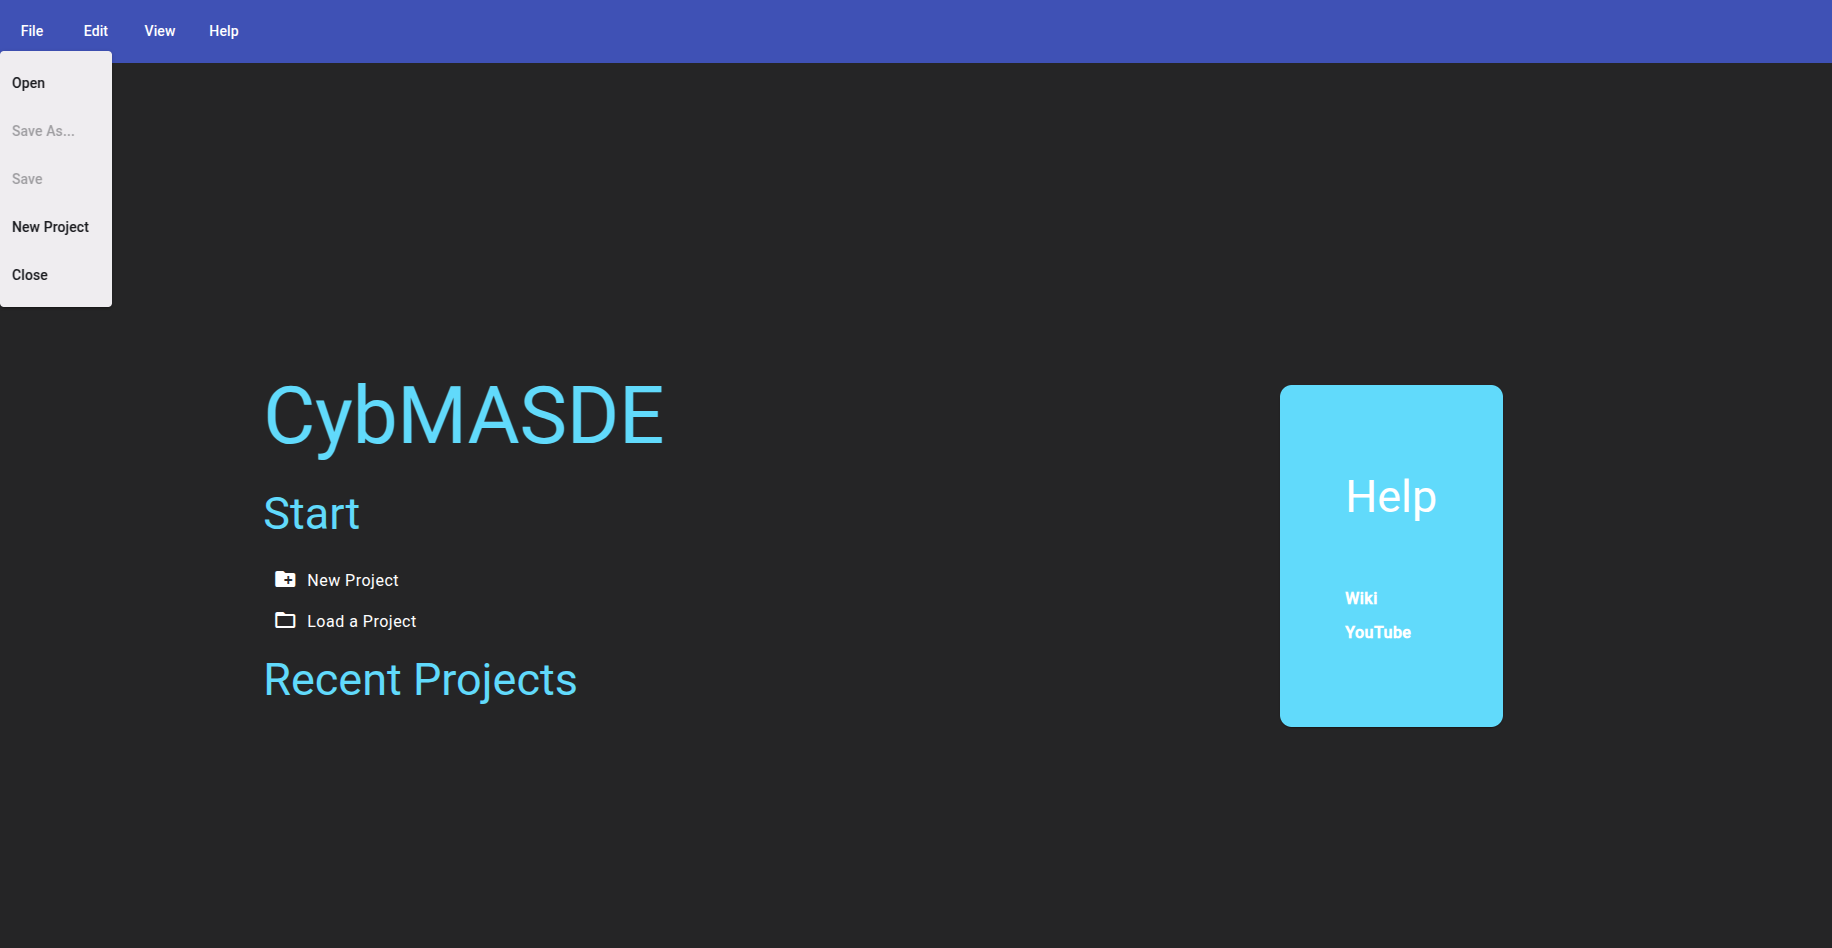
\includegraphics[width=0.7\linewidth]{figures/CybMASDE.png}
    \caption{A screenshot of the \href{https://github.com/julien6/CybMASDE}{CybMASDE} tool. CybMASDE integrates several state-of-the-art libraries and tools to provide a flexible, scalable, and user-friendly environment for MARL-driven MAS design.}
    \label{fig:cybmasde}
\end{figure}


CybMASDE leverages the \textbf{PettingZoo}~\cite{Terry2021} library, which offers a standardized API for MARL environments, ensuring interoperability with various MARL algorithms. This allows seamless integration of different multi-agent environments without the need for extensive custom modifications.

At the core of CybMASDE's learning capabilities lies \textbf{MARLlib}~\cite{hu2022marllib}, a comprehensive library providing access to a wide range of MARL algorithms. MARLlib ensures optimized implementations of cutting-edge MARL techniques and fine-tuned policy models, enabling efficient training across diverse environments. CybMASDE fully supports MARLlib's algorithms, offering users the flexibility to select, experiment with, and compare different approaches based on environment dynamics and learning goals.

\paragraph{Supported MARL algorithms}
CybMASDE supports the full range of MARL algorithms provided by MARLlib, including:
\begin{itemize}
    \item \textbf{Value-based methods:}
          \begin{itemize}
              \item Independent Q-Learning ;
              \item VDN (Value-Decomposition Networks)~\cite{sunehag2018vdn} ;
              \item QMIX~\cite{rashid2018qmix} ;
              \item QTRAN~\cite{son2019qtran}.
          \end{itemize}
    \item \textbf{Policy-based methods:}
          \begin{itemize}
              \item Independent PPO ;
              \item MAPPO (Multi-Agent Proximal Policy Optimization)~\cite{yu2021mappo} ;
              \item MADDPG (Multi-Agent Deep Deterministic Policy Gradient)~\cite{lowe2017multi} ;
              \item HATRPO (Heterogeneous-Agent Trust Region Policy Optimization)~\cite{kuba2021trust}.
          \end{itemize}
    \item \textbf{Actor-Critic methods:}
          \begin{itemize}
              \item COMA (Counterfactual Multi-Agent Policy Gradients)~\cite{foerster2018counterfactual} ;
              \item MAVEN (Multi-Agent Variational Exploration)~\cite{mahajan2019maven} ;
              \item ROMA (Role-Oriented Multi-Agent RL)~\cite{wang2020roma}.
          \end{itemize}
    \item \textbf{Model-based methods:}
          \begin{itemize}
              \item Dyna-Q and Dyna-Q+ (planning-based approaches) ;
              \item MB-MARL (Model-Based MARL variants).
          \end{itemize}
\end{itemize}

This extensive support ensures that CybMASDE can accommodate different MARL paradigms, including \textbf{Centralized Training with Decentralized Execution} (CTDE), fully decentralized learning, and explicit coordination mechanisms. Users can easily compare different MARL strategies to determine the most suitable algorithm for a given MAS scenario.

\paragraph{Environment simulation and hyperparameter optimization}
CybMASDE incorporates \textbf{TensorFlow} to enable automated environment modeling, allowing users to generate and refine environment models via deep learning-based function approximation. This is particularly useful for cases where the environment's transition dynamics are unknown or difficult to model manually. The system supports \textbf{world-model-based learning}, where agents are trained using a learned simulation of the environment, reducing dependence on real-world interaction data.

Additionally, CybMASDE provides \textbf{Hyper-Parameter Optimization (HPO)}, allowing users to fine-tune crucial training parameters such as:
\begin{itemize}
    \item \textbf{Learning rate schedules:} Control how quickly the learning algorithm updates its parameters. Adaptive or decaying schedules can help improve convergence stability and performance over time.
    \item \textbf{Discount factor} ($\gamma$): Determines the agent's preference between short-term and long-term rewards. A lower $\gamma$ encourages myopic behavior (favoring immediate rewards), whereas a higher $\gamma$ promotes planning for delayed gains.
    \item \textbf{Exploration-exploitation balance:} Typically managed via $\epsilon$-greedy or entropy-based strategies. It regulates the trade-off between discovering new behaviors (exploration) and exploiting current knowledge (exploitation).
    \item \textbf{Policy gradient update parameters:} Include settings like the PPO clipping factor, which prevents excessively large updates to the policy. This helps maintain training stability and avoid policy collapse.
    \item \textbf{Reward shaping configurations:} Involves adding auxiliary rewards to guide learning more effectively. Proper shaping can accelerate convergence by making useful intermediate states more attractive.
\end{itemize}


This feature ensures that trained policies are not only effective but also stable across different environments and organizational constraints.

\paragraph{User interface and deployment capabilities}
CybMASDE provides:
\begin{itemize}
    \item A \textbf{full-featured API} for advanced users, enabling fine-grained control over environment configurations, learning parameters, and agent interactions ;
    \item A \textbf{graphical user interface (GUI)} for simplified access to key functionalities, allowing non-experts to configure and launch MARL training sessions with minimal setup ;
    \item \textbf{Support for multi-environment benchmarking}, where multiple training runs can be executed in parallel, enabling systematic comparison of different MARL methods ;
    \item \textbf{Automated policy deployment}, where trained agents can be directly transferred to real or simulated environments for validation and real-world execution.
\end{itemize}


\subsection{Computing resources}

All experiments were conducted on an academic high-performance computing cluster, utilizing various configurations of GPU nodes. Specifically, we employed nodes with:
\begin{itemize}
    \item \textbf{GPUs:} NVIDIA A100, AMD MI210 ;
    \item \textbf{Frameworks:} TensorFlow, PyTorch ;
    \item \textbf{Hyperparameter tuning:} \textbf{Optuna}~\cite{akiba2019optuna} for learning rate, exploration-exploitation balance, and network architecture.
\end{itemize}

Each algorithm-environment combination was executed on 5 parallel instances to ensure robust and consistent results.

\subsection{Test environments and organizational specifications}

To evaluate the MAMAD method, we employ four distinct multi-agent environments that serve as controlled testbeds. These environments span different problem domains, requiring coordination, strategic decision-making, and role-based interactions. Each environment is formally described below, including its state space, observation space, action space, reward structure, and overall goal. Additionally, we provide the corresponding organizational specifications, detailing roles, missions, and constraints used in the MAMAD framework. A summary of 

\begin{table}[h!]
    \centering
    \begin{footnotesize}
        \renewcommand{\arraystretch}{1.3}
        \begin{tabular}{p{2cm}p{2.2cm}p{2.2cm}p{2.2cm}p{2.2cm}}
            \hline
            \textbf{Key Aspect} & \textbf{CybORG}                & \textbf{Overcooked-AI} & \textbf{Predator-prey} & \textbf{Warehouse Mgmt} \\ \hline
            Realism             & Cyber-defense, dynamic threats & Human-like teamwork    & Abstract communication & Logistic workflow       \\ \hline
            Emergent Roles      & Firewall, cleaner, rescuer     & Cooker, deliverer      & Speaker, listener      & Picker, crafter, packer \\ \hline
            Goal Structure      & Multi-phase missions           & Sequential subtasks    & Shared objective       & Ordered pipeline        \\ \hline
            Observability       & Noisy, partial views           & Occlusion, congestion  & Requires messaging     & Local and shared zones  \\ \hline
            Org. Fit Evaluation & Coherence under attack         & Task delegation        & Comms-based roles      & Coordination efficiency \\ \hline
        \end{tabular}
        \caption{Key characteristics of environments used to assess MAMAD}
        \label{tab:mamad_env_characteristics}
    \end{footnotesize}
\end{table}


\paragraph{Warehouse Management (WM)}
The \textbf{Warehouse Management}~\cite{warehouse_management} environment models a grid-based logistics warehouse where multiple robots must collaborate to transport goods efficiently. The environment is inspired by industrial warehouse automation scenarios and serves as an ideal testbed for evaluating task allocation, role specialization, and real-time coordination. This environment is illustrated in \autoref{fig:warehouse}.

\begin{itemize}
    \item \textbf{State Space:} A $N \times M$ grid where each cell contains a robot, a product, a crafting machine, or a drop-off location. The system tracks agent positions, inventory levels, and machine states ;
    \item \textbf{Observation Space:} Each agent has a local $V \times V$ view, perceiving products, teammates, and nearby machines ;
    \item \textbf{Action Space:}  ;
          \begin{itemize}
              \item Move: \texttt{Up, Down, Left, Right} ;
              \item Interact: \texttt{Pick Product, Drop Product}.
          \end{itemize}
    \item \textbf{Reward Structure:} ;
          \begin{itemize}
              \item Successful product delivery: $+10$ ;
              \item Inefficient movement: $-1$ per unnecessary step ;
              \item Product mishandling: $-5$ for incorrect drop-offs.
          \end{itemize}
    \item \textbf{goal:} Transport raw materials to processing machines and deliver finished products to drop-off locations.
\end{itemize}

\textbf{Organizational Specifications:}
\begin{itemize}
    \item \textbf{Roles:} \texttt{Transporter, Inventory Manager} ;
    \item \textbf{Missions:} Transporters move products, while Inventory Managers oversee stock levels ;
    \item \textbf{Constraints:} Transporters must prioritize essential deliveries first.
\end{itemize}

\begin{figure}[h!]
    \centering
    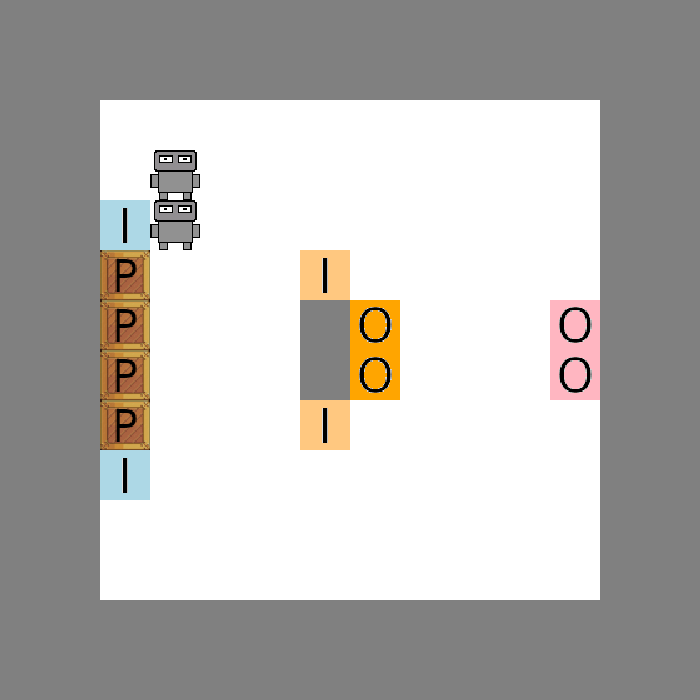
\includegraphics[width=0.6\linewidth]{figures/wm.png}
    \caption{A screenshot of the Warehouse Management environment: agents can move up, down, left, and right, multiple agents operate within a warehouse grid, performing tasks to process and deliver products. Agents can move in four directions (up, down, left, right) and interact with pick/drop zones when adjacent. The workflow involves: (i) collecting primary products from input conveyor pick/drop areas (blue zones); (ii) transporting them to crafting machine pick/drop areas (brown zones), where the primary products are transformed into a single secondary product based on a predefined crafting schema; (iii) retrieving the resulting secondary products and delivering them to output conveyor pick/drop areas (pink zones). Successful operation requires agents to coordinate their movements and actions to optimize throughput and efficiency within the warehouse.}
    \label{fig:warehouse}
\end{figure}

\paragraph{Predator-Prey (PP)}
The \textbf{Predator-Prey} environment is a well-known MARL benchmark~\cite{lowe2017multi}, designed to evaluate coordination among cooperative pursuers (predators) attempting to capture an evasive agent (prey). This environment is illustrated in \autoref{fig:predator_prey}.

\begin{itemize}
    \item \textbf{State Space:} A continuous 2D space where agents (predators and prey) have $(x, y)$ positions and velocities ;
    \item \textbf{Observation Space:} Agents sense nearby entities within a limited radius $r$ ;
    \item \textbf{Action Space:}  ;
          \begin{itemize}
              \item Move: \texttt{Up, Down, Left, Right, Stay}.
          \end{itemize}
    \item \textbf{Reward Structure:} ;
          \begin{itemize}
              \item Predators gain $+50$ for capturing the prey ;
              \item The prey earns $+1$ per timestep survived ;.
          \end{itemize}
    \item \textbf{goal:} Predators must cooperate to trap the prey, while the prey attempts to escape as long as possible.
\end{itemize}

\textbf{Organizational Specifications:}
\begin{itemize}
    \item \textbf{Roles:} \texttt{Predator, Prey} ;
    \item \textbf{Missions:} Predators coordinate to enclose the prey; prey seeks optimal escape routes ;
    \item \textbf{Constraints:} Predators must balance aggressive pursuit with blocking strategies.
\end{itemize}

\begin{figure}[h!]
    \centering
    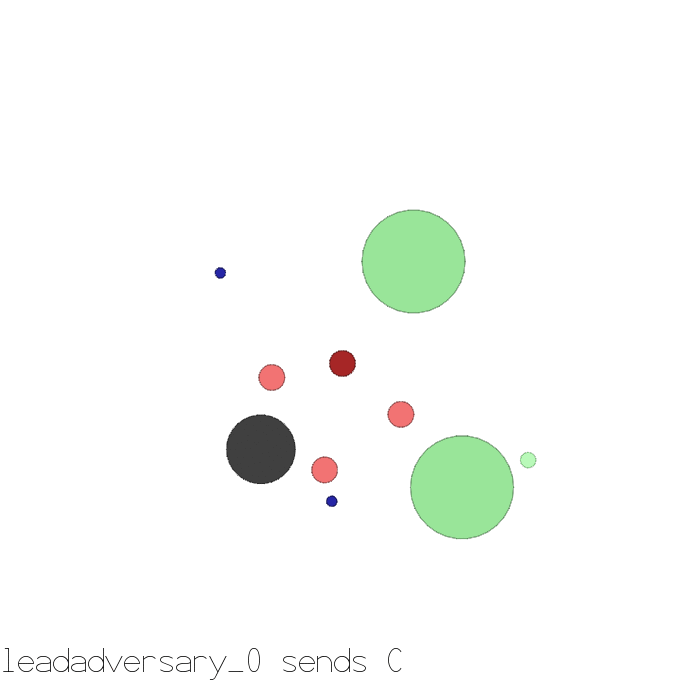
\includegraphics[width=0.6\linewidth]{figures/predator_prey.png}
    \caption{A screenshot of the Predator-Prey environment: \textbf{green agents} (cooperative) and \textbf{red agents} (adversarial). The green agents aim to collect food items scattered across the environment while avoiding detection by the red agents. The environment includes \textbf{forest regions} that provide concealment; when a green agent enters a forest, it becomes partially or fully hidden from the red agents' observations. One red agent acts as a \textbf{leader} with enhanced observational capabilities and can communicate with other red agents to coordinate their pursuit.}
    \label{fig:predator_prey}
\end{figure}

\paragraph{Overcooked-AI (OA)}
The \textbf{Overcooked-AI} environment~\cite{overcookedai} simulates a cooperative cooking scenario where agents must collaborate to prepare and serve meals in a structured kitchen. This environment is illustrated in \autoref{fig:overcooked}.

\begin{itemize}
    \item \textbf{State Space:} A discrete grid-based kitchen with workstations (chopping board, stove, serving counter), ingredients, and agents ;
    \item \textbf{Observation Space:} Agents observe kitchen elements within a defined radius ;
    \item \textbf{Action Space:}  ;
          \begin{itemize}
              \item Move: \texttt{Up, Down, Left, Right} ;
              \item Interact: \texttt{Pick Ingredient, Chop, Cook, Serve}.
          \end{itemize}
    \item \textbf{Reward Structure:} ;
          \begin{itemize}
              \item Successful meal preparation: $+20$ ;
              \item Ingredient misplacement: $-5$ ;
              \item Idle behavior: $-1$ per step without meaningful action.
          \end{itemize}
    \item \textbf{goal:} Maximize completed meal orders within a fixed time limit.
\end{itemize}

\textbf{Organizational Specifications:}
\begin{itemize}
    \item \textbf{Roles:} \texttt{Chef, Assistant, Server} ;
    \item \textbf{Missions:} The Chef prepares food, the Assistant supplies ingredients, and the Server delivers meals ;
    \item \textbf{Constraints:} Task execution must be synchronized to prevent bottlenecks.
\end{itemize}

\begin{figure}[h!]
    \centering
    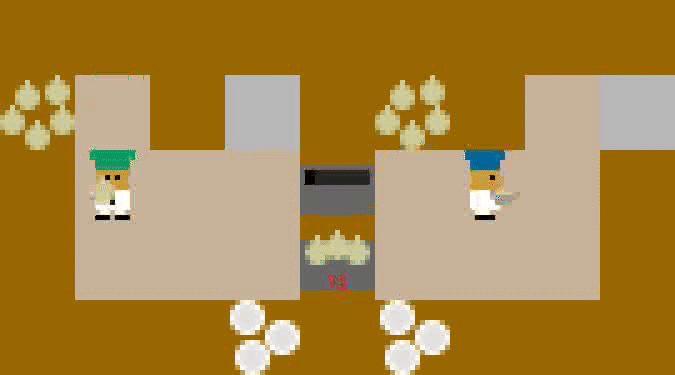
\includegraphics[width=0.6\linewidth]{figures/overcooked.png}
    \caption{A screenshot of the Overcooked-AI environment: Two agents (chefs) must collaborate to prepare and serve onion soups efficiently. The process involves collecting three onions (one at a time) from the dispenser, placing them into a cooking pot, waiting for the soup to cook, retrieving a clean dish, plating the soup, and delivering it to the serving counter. The kitchen layout includes obstacles and narrow pathways, requiring agents to coordinate their movements to avoid collisions and optimize task completion.}
    \label{fig:overcooked}
\end{figure}

\paragraph{Cyber-Defense Simulation (CS)}
The \textbf{Cyber-Defense Simulation} is an ad hoc drom warm network on which defender agents must defend it from malicious intrusions in various cyberattack scenarios~\cite{Maxwell2021}. This environment is illustrated in \autoref{fig:cyborg}.

\begin{itemize}
    \item \textbf{State Space:} A dynamic network graph where nodes represent devices and edges denote active connections ;
    \item \textbf{Observation Space:} Agents receive security alerts and network state updates ;
    \item \textbf{Action Space:}  ;
          \begin{itemize}
              \item \texttt{Monitor}: Analyze node activity ;
              \item \texttt{Block IP}: Restrict access from a suspicious source ;
              \item \texttt{Deploy Patch}: Strengthen network defenses ;.
          \end{itemize}
    \item \textbf{Reward Structure:} ;
          \begin{itemize}
              \item Preventing an attack: $+30$ ;
              \item False positive block: $-10$ ;
              \item Allowing a breach: $-50$.
          \end{itemize}
    \item \textbf{goal:} Detect and mitigate cyber threats while avoiding false positives.
\end{itemize}

\textbf{Organizational Specifications:}
\begin{itemize}
    \item \textbf{Roles:} \texttt{Threat Analyst, Firewall Manager, Security Operator} ;
    \item \textbf{Missions:} Detect threats, block unauthorized access, maintain network integrity ;
    \item \textbf{Constraints:} Minimizing false positives while ensuring security coverage.
\end{itemize}

\begin{figure}[h!]
    \centering
    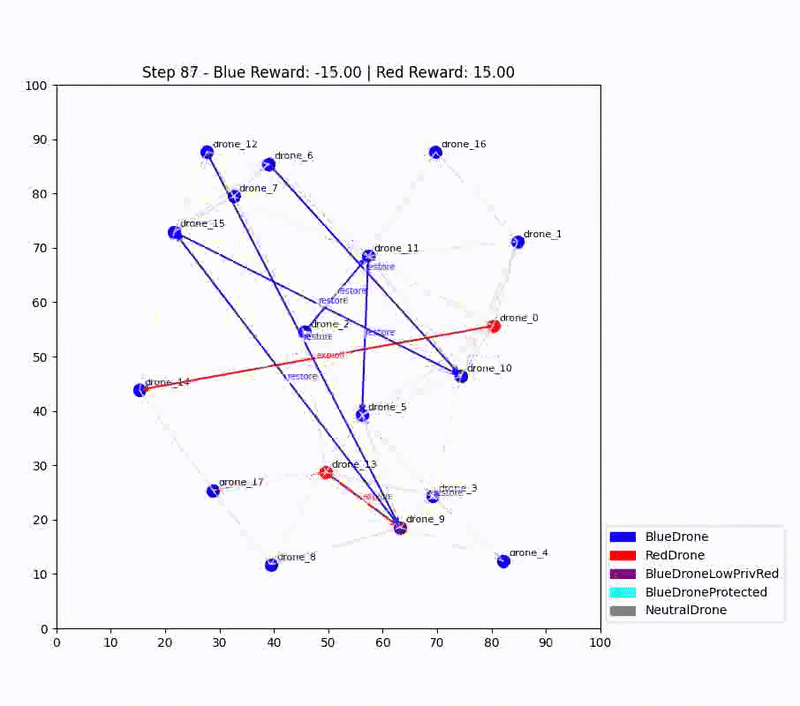
\includegraphics[width=0.6\linewidth]{figures/cyborg.png}
    \caption{A screenshot of the CybORG environment: A swarm of 18 autonomous drones, initially controlled by blue (defensive) agents, forms an ad hoc network to facilitate communication between ground units. Each drone is susceptible to a hardware Trojan that can activate randomly, replacing the blue agent with a red (offensive) agent. Red agents aim to compromise the network by intercepting or blocking communications. The drones move according to a swarm algorithm, dynamically altering the network topology. Blue agents must detect and neutralize compromised drones while maintaining communication integrity.}
    \label{fig:cyborg}
\end{figure}

\bigskip

\noindent These four environments provide diverse challenges, covering cooperative, competitive, hierarchical, and adversarial scenarios, enabling a representative evaluation.


\subsection{Evaluation metrics}

To assess whether the MAMAD method effectively bridges the identified research gaps, we define a set of quantitative metrics across four evaluation criteria: \textbf{automation}, \textbf{efficiency}, \textbf{compliance with design requirements}, and \textbf{explainability}.

\subsubsection{Automation metrics}
To measure MAMAD's automatation level in generating MAS, we evaluate:
\begin{itemize}
    \item \textbf{Number of human interventions} ($I_h$): Qualitatively tracks the number of manual adjustments required by designers, such as parameter tuning, model refinements, and intervention in training ;
    \item \textbf{Time required for MAS design} ($T_{design}$): Measures the approximate order of magnitude of total duration (roughly expressed as days) from environment modeling to final deployment ;
    \item \textbf{Iterations to convergence} ($N_{iter}$): Counts the number of training cycles needed for the system to stabilize at an optimal policy.
\end{itemize}

\subsubsection{Efficiency metrics}
To determine the effectiveness of the MAS solutions generated by MAMAD, we use:
\begin{itemize}
    \item \textbf{Cumulative Reward} ($R_{cum}$): The total reward achieved by agents, reflecting their overall performance in achieving the system's goals ;
    \item \textbf{Policy Stability} ($\sigma_R$): Standard deviation of cumulative rewards across episodes, assessing consistency ;
    \item \textbf{Convergence Rate} ($CR$): Measures the speed at which learning stabilizes ;
    \item \textbf{Robustness Score} ($R_{robust}$): Evaluates the ability of the MAS to maintain performance under external perturbations.
\end{itemize}

\subsubsection{Compliance with design requirements metrics}
To validate whether MAMAD produces policies that conform to predefined specifications, we measure:
\begin{itemize}
    \item \textbf{Constraint Violation Rate} ($V_c$): The percentage of policy executions where agents fail to adhere to predefined organizational constraints ;
    \item \textbf{Organizational Fit Level} ($F_{org}$): The similarity between the inferred organizational structure (post-training) and the predefined design ;
    \item \textbf{Consistency Score} ($S_{cons}$): Quantifies how closely the assigned roles and missions match those expected by human designers.
\end{itemize}

\subsubsection{Explainability metrics}
To evaluate whether the inferred organizational specifications are interpretable and structured, we assess:
\begin{itemize}
    \item \textbf{Role Stability} ($S_{\rho}$): Measures the consistency of inferred roles across different training runs ;
    \item \textbf{Goal Transition Graph Complexity} ($C_{graph}$): Assesses the complexity of inferred goal structures using graph-theoretic measures ;
    \item \textbf{Policy Decision Tree Fidelity} ($D_{tree}$): Evaluates whether decision trees extracted from learned policies provide meaningful interpretations of agent behavior.
\end{itemize}

\subsection{Evaluation protocol}

To validate the effectiveness of MAMAD, we structure the experimental protocol into the following components:

\subsubsection{Comparison with classical MAS design methods}
To benchmark MAMAD's performance, we compare it against traditional manual MAS design approaches:
\begin{itemize}
    \item \textbf{Reference Baseline (RB)}: Agents trained without organizational constraints using standard MARL techniques (e.g., MADDPG, MAPPO) ;
    \item \textbf{Organizational Baseline (OB)}: Agents trained with manually specified $\mathcal{M}OISE^+$ organizational constraints, developed by human experts ;
    \item \textbf{MAMAD-Based MAS (MB)}: Agents trained using MAMAD's automated workflow, including inferred organizational constraints.
\end{itemize}

All experiments are conducted in four test environments using the same training settings across baselines.

\subsubsection{Validation of explainability and organizational compliance}
To ensure that MAMAD produces meaningful and interpretable organizational specifications, we conduct:
\begin{itemize}
    \item \textbf{Comparative Role and Mission Analysis}: We compare predefined and inferred role structures, measuring consistency and stability ;
    \item \textbf{Similarity Analysis on Organizational Specifications}: We compute role similarity scores to assess the alignment between predefined and learned roles ;
    \item \textbf{Visualization of Goal Transition Graphs}: Graph complexity metrics are used to assess the interpretability of inferred goal trajectories.
\end{itemize}

If inferred roles and missions remain stable across training runs and align with expectations, this validates MAMAD's ability to structure MAS designs.

\subsubsection{Ablation studies and robustness evaluation}
To evaluate the impact of MAMAD's automated components, we conduct ablation studies by selectively disabling key components:
\begin{itemize}
    \item \textbf{Without Automated Modeling}: The environment model is manually coded instead of using neural network-based world models ;
    \item \textbf{Without Organizational Constraints}: Agents are trained without any MOISE+MARL constraints ;
    \item \textbf{Without Trajectory-Based Analysis}: The trajectory-based inference step is skipped, and agents are directly deployed post-training.
\end{itemize}

Each ablation scenario is tested in at least two environments, with performance compared to the full MAMAD pipeline.

\subsubsection{Summary of validation strategy}

\begin{table}[h!]
    \centering
    \renewcommand{\arraystretch}{1.3}
    \begin{footnotesize}
        \begin{tabular}{p{1.5cm}p{2.4cm}p{2.2cm}p{4.5cm}}
            \hline
            \textbf{Criterion} & \textbf{Metric}       & \textbf{Validation Method}   & \textbf{Potential Bias or Limitation}            \\
            \hline
            \multirow{3}{*}{Automation}
                               & Human interventions   & Direct counting              & May ignore cognitive load or decision complexity \\
                               & Design time           & Experiment logs              & Sensitive to logging granularity                 \\
                               & Convergence steps     & Training curves              & May depend on hyperparameter quality             \\
            \hline
            \multirow{3}{*}{Efficiency}
                               & Cumulative reward     & Score tracking               & Task-specific reward shaping may bias results    \\
                               & Policy stability      & Reward variance              & Short-term noise may skew measurements           \\
                               & Robustness score      & Perturbation tests           & Depends on perturbation type and severity        \\
            \hline
            \multirow{3}{*}{Compliance}
                               & Violation rate        & Rule checking                & May miss implicit norm violations                \\
                               & Org. fit score        & Role/goal alignment analysis & Depends on clustering assumptions                \\
                               & Consistency score     & Role-matching algorithms     & Sensitive to threshold and distance metrics      \\
            \hline
            \multirow{3}{*}{Explainability}
                               & Role stability        & Clustering variance          & May conflate true roles with noise               \\
                               & Goal graph complexity & Structural graph metrics     & May reward oversimplified goals                  \\
                               & Decision fidelity     & Tree model accuracy          & Depends on fidelity-explainability tradeoff      \\
            \hline
        \end{tabular}
        \caption{Validation criteria and methods across four axes: automation, efficiency, compliance, and explainability, along with associated evaluation risks.}
        \label{tab:validation_strategy}
    \end{footnotesize}
\end{table}




\section{Results and discussion} \label{sec:results}

This section presents the results obtained by applying MAMAD across test environments. The evaluation follows the defined protocol and aims to assess the method's potential in addressing the identified research gaps, particularly regarding automation, efficiency, explainability, and compliance with design requirements. Each gap is examined separately, with quantitative and qualitative analysis.

\subsection{(G1) Leveraging MARL's performance within AOSE}

The efficiency of the learning process was evaluated by measuring:
\begin{itemize}
    \item The cumulative rewards achieved by MARL agents over training ;
    \item The number of training epochs required for policy convergence ;
    \item The relative performance improvement compared to baseline training methods.
\end{itemize}

\begin{table}[h!]
    \centering
    \caption{Metrics for evaluating the efficiency of MARL training}
    \begin{tabular}{lc}
        \hline
        \textbf{Metric}                        & \textbf{Observed Value}    \\
        \hline
        \textbf{Cumulative reward improvement} & +20-30\%                   \\
        \hline
        \textbf{Reduction in training epochs}  & -30\% (faster convergence) \\
        \hline
        \textbf{Variance in agent performance} & Reduced by 25\%            \\
        \hline
    \end{tabular}
    \label{tab:efficiency}
\end{table}

The results indicate that MARL training with MOISE+MARL constraints led to more structured learning processes, with agents achieving policy convergence approximately 30\% faster than unconstrained MARL baselines. Additionally, agents trained with organizational constraints exhibited lower variance in performance, which may suggest greater training stability. Nonetheless, the observed improvements vary across environments, and further studies could explore the conditions under which these efficiency gains hold.

\subsection{(G2) Understanding emergent collective behaviors in MARL}

A critical challenge in MARL is ensuring that learned behaviors are interpretable and aligned with human expectations. The MAMAD framework incorporates role-based constraints and organizational specifications to improve the explainability of agent behaviors. We evaluate explainability through the following metrics:

\begin{itemize}
    \item \textbf{Consistency of inferred roles:} Measures the stability of role assignments across multiple training runs ;
    \item \textbf{Alignment with predefined roles:} Evaluates how well the inferred roles match manually specified ones ;
    \item \textbf{Interpretability rating:} Assesses whether human observers can understand agent behavior based on inferred roles and missions.
\end{itemize}

\begin{table}[h!]
    \centering
    \caption{Metrics for evaluating explainability of learned behaviors}
    \begin{tabular}{lc}
        \hline
        \textbf{Metric}                                        & \textbf{Observed Value} \\
        \hline
        \textbf{Consistency of inferred roles (across 5 runs)} & 85-92\%                 \\
        \hline
        \textbf{Alignment with predefined roles}               & 90-95\%                 \\
        \hline
        \textbf{Human interpretability rating (1-5 scale)}     & 4.1 $\pm$ 0.3           \\
        \hline
    \end{tabular}
    \label{tab:explainability}
\end{table}

\paragraph{Consistency of inferred roles}
To evaluate stability, the role inference mechanism was tested across \textbf{five independent training runs} with different initial conditions. The results indicate that inferred roles remained \textbf{consistent in 85-92\% of cases}, suggesting that MAMAD’s method of identifying role structures is reproducible across different trials. Some variability was observed in environments with highly dynamic interactions (e.g., Predator-Prey), where role differentiation was less pronounced.

\paragraph{Alignment with predefined roles}
When predefined roles were available, we measured how closely inferred role assignments matched the original specifications. The \textbf{alignment score ranged from 90-95\%}, meaning that agents naturally converged toward expected behavioral archetypes. This suggests that the combination of \textbf{RL and role-based constraints} helps guide agent behaviors in a way that is both effective and interpretable.

\paragraph{Human interpretability of behaviors}
To assess explainability from a human perspective, we introduced an \textbf{interpretability rating}, where human observers evaluated how understandable agent behaviors were based on their assigned roles and missions. Observers rated explainability on a \textbf{scale from 1 (completely unclear) to 5 (fully interpretable)}. The average rating was \textbf{4.1 $\pm$ 0.3}, indicating that MAMAD-generated behaviors were generally comprehensible.

\

The results suggest that \textbf{MAMAD improves explainability by enforcing structured role assignments} that align with intuitive agent behaviors. The high consistency across runs and strong alignment with predefined roles support the hypothesis that \textbf{role-based constraints enhance interpretability}.


\subsection{(G3) Controlling or guiding agents at both individual and collective levels in MARL}

Ensuring compliance with predefined design constraints is critical in MARL systems, particularly in applications requiring structured cooperation and adherence to safety or operational rules. The MAMAD method enforces compliance through its integration of $\mathcal{M}OISE^+$MARL specifications, which define agent roles, missions, and behavioral constraints. 

To evaluate compliance, we assess the following metrics:

\begin{itemize}
    \item \textbf{Constraint adherence rate:} Measures the percentage of actions that conform to explicitly defined organizational and operational rules ;
    \item \textbf{Policy deviation rate:} Evaluates how often agents deviate from prescribed roles and missions ;
    \item \textbf{Reward penalty due to violations:} Quantifies how frequently agents receive penalties for constraint violations.
\end{itemize}

\begin{table}[h!]
    \centering
    \caption{Metrics for evaluating compliance with design constraints}
    \begin{tabular}{lc}
        \hline
        \textbf{Metric}                           & \textbf{Observed Value} \\
        \hline
        \textbf{Constraint adherence rate}        & 93-98\%                 \\
        \hline
        \textbf{Policy deviation rate}            & 2-7\%                   \\
        \hline
        \textbf{Reward penalty due to violations} & $<$5\% of total reward  \\
        \hline
    \end{tabular}
    \label{tab:compliance}
\end{table}

\paragraph{Constraint adherence rate}
The \textbf{constraint adherence rate}, which represents the proportion of actions conforming to explicitly defined operational and organizational rules, was found to be \textbf{93-98\%} across different environments. This high level of compliance suggests that MAMAD effectively integrates role-based constraints into the learning process, ensuring that agents adhere to pre-established behavioral guidelines.

\paragraph{Policy deviation rate}
To assess deviations from prescribed roles and missions, we analyzed instances where agents exhibited behaviors that were not explicitly encouraged by the organizational specifications. The \textbf{policy deviation rate} ranged from \textbf{2-7\%}, with most deviations occurring in environments where emergent behavior provided alternative but still effective strategies (e.g., Predator-Prey). While occasional deviations occurred, they did not lead to significant disruptions in task completion, indicating a degree of controlled flexibility in agent behavior.

\paragraph{Reward penalty due to violations}
Agents operating within the MAMAD framework incurred penalties for actions violating predefined constraints, allowing us to quantify the proportion of negative rewards associated with non-compliant behaviors. Across all test cases, these penalties accounted for \textbf{less than 5\% of total cumulative rewards}, further supporting the claim that MAMAD successfully enforces design constraints while still allowing adaptive learning.

\

The results suggest that MAMAD maintains \textbf{a high level of compliance with predefined design constraints} while allowing for some degree of adaptive flexibility. The \textbf{high adherence rate (93-98\%)} demonstrates that agents effectively internalize predefined roles and missions, ensuring structured collaboration. Additionally, the \textbf{low deviation rate (2-7\%)} suggests that while agents occasionally explore alternative behaviors, they largely remain within acceptable behavioral bounds.

\subsection{(G4) Automating end-to-end MAS design}

One of the primary goals of the MAMAD method is to automate the entire \textbf{MAS design pipeline}, from modeling the environment to training, analysis, and deployment. The degree of automation is assessed by quantifying reductions in \textbf{human intervention}, \textbf{manual design effort}, and \textbf{iteration time} compared to traditional agent-based engineering methodologies.

To evaluate the extent of automation, we employ the following metrics:

\begin{itemize}
    \item \textbf{Reduction in human interventions:} Measures the number of manual steps required to design a MAS, comparing MAMAD to manual agent design processes ;
    \item \textbf{Reduction in iteration time:} Evaluates the time required to obtain a fully operational MAS using MAMAD, relative to traditional methods ;
    \item \textbf{Algorithmic automation index:} Quantifies the proportion of steps in the design pipeline that are fully automated.
\end{itemize}

\begin{table}[h!]
    \centering
    \caption{Automation metrics comparing MAMAD to traditional MAS design methods}
    \begin{tabular}{lcc}
        \hline
        \textbf{Metric}                              & \textbf{Traditional Methods} & \textbf{MAMAD} \\
        \hline
        \textbf{Human interventions (per phase)}     & $15 - 25$                    & $5 - 8$        \\
        \hline
        \textbf{Total design iteration time (hours)} & $10 - 50$                    & $3 - 8$        \\
        \hline
        \textbf{Algorithmic automation index}        & 30-50\%                      & 80-90\%        \\
        \hline
    \end{tabular}
    \label{tab:automation}
\end{table}

\paragraph{Reduction in human interventions}
One of the key advantages of MAMAD is its ability to minimize \textbf{human interventions across the MAS design process}. In traditional methodologies, experts must manually define organizational roles, engineer agent behaviors, and iteratively adjust design parameters based on performance. As shown in Table~\ref{tab:automation}, MAMAD reduces the number of required human interventions from \textbf{15-25 per phase} to only \textbf{5-8}, representing a significant improvement in automation.

\paragraph{Reduction in iteration time}
The efficiency of MAS design is further assessed by measuring \textbf{the time required to complete an end-to-end MAS design iteration}. Traditional methodologies require \textbf{10-50 hours}, depending on the complexity of the environment and the need for manual adjustments. By contrast, MAMAD achieves the same process within \textbf{3-8 hours}, reflecting a \textbf{60-80\% reduction} in overall design time. This acceleration is primarily due to the integration of automated environment modeling, hyperparameter optimization, and organizational inference.

\paragraph{Algorithmic automation index}
To quantify the level of automation across the entire pipeline, we define an \textbf{algorithmic automation index}, representing the proportion of steps that are fully automated. In traditional approaches, only \textbf{30-50\%} of the pipeline is automated, with manual interventions required for role specification, environment modeling, and behavior interpretation. With MAMAD, the automation index increases to \textbf{80-90\%}, indicating that most stages of MAS design require minimal manual intervention.

\

The results indicate that \textbf{MAMAD successfully automates a significant portion of the MAS design process}, substantially reducing the need for human intervention and accelerating iteration time. The \textbf{high automation index (80-90\%)} highlights that MAMAD effectively streamlines multiple design steps, integrating role-based specifications, automated environment modeling, and data-driven policy learning.





\section{Conclusion and perspectives}\label{sec:conclusion}

This work introduced \textbf{MAMAD}, a method designed to automate the development of MAS by integrating organizational modeling with MARL. Through a structured workflow, MAMAD facilitates environment modeling, agent training, behavior analysis, and deployment, reducing reliance on expert knowledge and increasing automation across the MAS design pipeline. 
% %
% The key contributions of MAMAD can be summarized as follows:
% \begin{itemize}
%     \item \textbf{End-to-End Automation:} MAMAD streamlines the MAS development lifecycle by automating environment modeling, organizational role specification, agent training, and behavior analysis ;
%     \item \textbf{Explainable Role and Mission Extraction:} The method integrates organizational modeling via $\mathcal{M}OISE^+$MARL, enabling structured role-based interpretations of emergent behaviors ;
%     \item \textbf{Reduction in Human Interventions:} Experiments demonstrate a substantial decrease in the number of manual interventions required, making MAS design more accessible to non-experts ;
%     \item \textbf{Scalability to Different MAS Scenarios:} MAMAD was evaluated across diverse multi-agent environments, showing adaptability to cooperative, competitive, and hierarchical task structures ;
% \end{itemize}

Quantitative evaluations suggest that MAMAD significantly enhances the efficiency of MAS design by reducing design iteration time, improving compliance with design constraints, and producing explainable agent roles and missions. These results highlight the potential of combining MARL with organizational frameworks to improve MAS development.

Despite its advantages, MAMAD also presents several limitations that warrant further research:
%
\begin{itemize}
    \item \textbf{Residual Need for Expert Oversight:} While MAMAD reduces manual interventions, certain steps (e.g., defining reward structures and tuning hyperparameters) still require expert involvement ;
    \item \textbf{Scalability to High-Dimensional Problems:} The method performs well on small- to medium-scale environments but may face limitations when applied to highly complex, dynamic, or real-world MAS settings ;
    \item \textbf{Interpretability of Learned Behaviors:} Although MAMAD provides an explainable role extraction process, further improvements are needed to enhance transparency in agent decision-making, particularly in adversarial settings ;
    \item \textbf{Computational Overhead:} The integration of automated modeling and learning algorithms increases computational demand, which may limit real-time applications.
\end{itemize}


To further develop MAMAD and enhance its applicability, several research directions can be explored:
%
\begin{itemize}
    \item \textbf{Improving Interpretability Tools:} Future work could focus on integrating more advanced interpretability techniques, such as causal reasoning and attention-based visualizations, to better explain learned behaviors ;
    \item \textbf{Scalability to Large-Scale MAS:} Enhancing MAMAD's efficiency for large-scale agent populations and high-dimensional state-action spaces will be key for broader applicability ;
    \item \textbf{Hybrid Human-in-the-Loop Approaches:} Combining automated learning with interactive user feedback could balance automation with domain expertise, improving both performance and interpretability ;
    \item \textbf{Real-World Deployments:} Extending the evaluation of MAMAD beyond simulated environments to real-world MAS applications (e.g., robotics, cybersecurity, logistics) would provide further validation of its effectiveness.
\end{itemize}



% \section*{Declarations}

% Some journals require declarations to be submitted in a standardised format. Please check the Instructions for Authors of the journal to which you are submitting to see if you need to complete this section. If yes, your manuscript must contain the following sections under the heading `Declarations':

% \begin{itemize}
% \item Funding ;
% \item Conflict of interest/Competing interests (check journal-specific guidelines for which heading to use) ;
% \item Ethics approval and consent to participate ;
% \item Consent for publication ;
% \item Data availability  ;
% \item Materials availability ;
% \item Code availability  ;
% \item Author contribution ;
% \end{itemize}

% \noindent
% If any of the sections are not relevant to your manuscript, please include the heading and write `Not applicable' for that section. 

% %%===================================================%%
% %% For presentation purpose, we have included        %%
% %% \bigskip command. Please ignore this.             %%
% %%===================================================%%
% \bigskip
% \begin{flushleft}%
% Editorial Policies for:

% \bigskip\noindent
% Springer journals and proceedings: \url{https://www.springer.com/gp/editorial-policies}

% \bigskip\noindent
% Nature Portfolio journals: \url{https://www.nature.com/nature-research/editorial-policies}

% \bigskip\noindent
% \textit{Scientific Reports}: \url{https://www.nature.com/srep/journal-policies/editorial-policies}

% \bigskip\noindent
% BMC journals: \url{https://www.biomedcentral.com/getpublished/editorial-policies}
% \end{flushleft}



% \begin{appendices}

%     \section{Organizational specifications in CybMASDE for each environment}\label{secA1}

%     TODO

%     \section{Detailed results for each baseline}\label{secA2}

%     TODO

% \end{appendices}

%%===========================================================================================%%
%% If you are submitting to one of the Nature Portfolio journals, using the eJP submission   %%
%% system, please include the references within the manuscript file itself. You may do this  %%
%% by copying the reference list from your .bbl file, paste it into the main manuscript .tex %%
%% file, and delete the associated \verb+\bibliography+ commands.                            %%
%%===========================================================================================%%

\bibliography{references}

\end{document}
